\documentclass[11pt,a4paper,twoside]{tesis}
% SI NO PENSAS IMPRIMIRLO EN FORMATO LIBRO PODES USAR
%\documentclass[11pt,a4paper]{tesis}

\usepackage[toc,page]{appendix}

\usepackage{color}
\usepackage{array}
\usepackage{tikz}
\usepackage{tikz-qtree}
\usetikzlibrary{positioning}
\usetikzlibrary{babel}
\usepackage[T1]{fontenc}
\usepackage{longtable}
\usepackage{graphicx}
\usepackage{float} % para settear posicion a imagenes
\usepackage[utf8]{inputenc}
\usepackage[spanish]{babel}
\usepackage[left=3cm,right=3cm,bottom=3.5cm,top=3.5cm]{geometry}
\usepackage{hyperref} %Para poner link en toc. Creo que tambien para los hrefs en azul
\hypersetup{colorlinks,    citecolor=black,    filecolor=black,    linkcolor=red,    urlcolor=black}
\usepackage{multirow}
\usepackage{bookmark}
%\usepackage{titlesec}
%\usepackage{sectsty}
\usepackage{amsmath}
\usepackage{amssymb}
\usepackage{rotating} % to rotate table in 4

%header configuration
\usepackage{titlesec}%Para configurar el formato de los headers (section, subsection, etc)

\titleformat*{\section}{\LARGE\bfseries}
\titleformat*{\subsection}{\Large\bfseries}
\titleformat*{\subsubsection}{\large\bfseries}
\titleformat*{\paragraph}{\large\bfseries}
\titleformat*{\subparagraph}{\large\bfseries}
%end header configuration

%\subsubsectionfont{\large}

\setcounter{tocdepth}{4} % Si se muestra subsubsection o no en el toc
\setcounter{secnumdepth}{4}

\newcommand\dblquote[1]{\textquotedblleft #1\textquotedblright}
\newcommand\sglquote[1]{\textquoteleft #1\textquoteright}
\newcommand\dq[1]{\textquotedblleft #1\textquotedblright}
\newcommand\sq[1]{\textquoteleft #1\textquoteright}



\newcommand*{\allref}[1]{\ref{#1} \nameref{#1}}
\newcommand*{\cerrada}{{\color{green}Cerrada}\newline}
\newcommand*{\cerradaarg}[1]{{\color{green}#1}\newline}
\newcommand*{\falta}{{\color{red}Falta bastante}\newline}
\newcommand*{\horrible}{{\color{red}Horrible}\newline}
\newcommand*{\bienahi}{{\color{green}Bien hasta ahí}\newline}
\newcommand*{\horriblearg}[1]{{\color{red}#1}\newline}
\newcommand*{\faltapoco}{{\color{yellow}Falta poco}\newline}
\newcommand*{\faltadependiente}{{\color{yellow}Faltan cosas que dependen de otras cosas}\newline}

\newcommand*{\tradqd}{$q-traduccion$}

\renewcommand{\appendixname}{Apéndices}
\renewcommand{\appendixtocname}{Apéndices}
\renewcommand{\appendixpagename}{Apéndices}
%\usepackage[nottoc,numbib]{tocbibind}

\begin{document}

%%%% CARATULA
\def\autor{Julián Peller}
\def\titulo{Question answering de dominio abierto y dominio cerrado}
\def\runtitulo{Question answering de dominio abierto y dominio cerrado}
\def\runtitle{Question answering de dominio abierto y dominio cerrado}
\def\director{José Castaño}
%\def\codirector{Master Yoda}
\def\lugar{Buenos Aires, 2015}
\newcommand{\HRule}{\rule{\linewidth}{0.2mm}}
%
\thispagestyle{empty}

\begin{center}\leavevmode

\vspace{-2cm}

\begin{tabular}{l}

\includegraphics[width=2.6cm]{logofcen.pdf}
\end{tabular}


{\large \sc Universidad de Buenos Aires

Facultad de Ciencias Exactas y Naturales

Departamento de Computaci\'on}

\vspace{6.0cm}

%\vspace{3.0cm}
%{
%\Large \color{red}
%\begin{tabular}{|p{2cm}cp{2cm}|}
%\hline
%& Pre-Final Version: \today &\\
%\hline
%\end{tabular}
%}
%\vspace{2.5cm}

{\huge\bf \titulo}

\vspace{2cm}

{\large Tesis presentada para optar al t\'{\i}tulo de\\
Licenciado en Ciencias de la Computaci\'on}

\vspace{2cm}

{\Large \autor}

\end{center}

\vfill

{\large

{Director: \director}

\vspace{.2cm}

%{Codirector: \codirector}

%\vspace{.2cm}

\lugar
}

\newpage\thispagestyle{empty}


%%%% ABSTRACTS, AGRADECIMIENTOS Y DEDICATORIA
\frontmatter
\pagestyle{empty}
%\begin{center}
%\large \bf \runtitulo
%\end{center}
%\vspace{1cm}
\chapter*{\runtitulo}
Question answering es un área de ciencias de la computación que busca generar respuestas concretas a preguntas expresadas en algún lenguaje natural. Es un área compleja que combina herramientas de búsqueda y recuperación de la información (\textit{information retrieval}), de procesamiento del lenguaje natural (\textit{nlp}) y de extracción de información (\textit{information extraction}). Por poner un ejemplo: para el input \textit{\dq{?`Cuándo nació Noam Chomsky?}} un sistema de question answering debería devolver algo como \dq{\textit{el 7 de diciembre de 1928}}.
Este área representa el paso lógico posterior a los sistemas de recuperación de documentos y logró en los último años una serie de hitos impulsados por el proyecto general de la web semántica. Watson, el sistema desarrollado por IBM que derrotó a los mejores competidos de Jeropardy! es el ejemplo más visible, pero incluso buscadores como Bing! y Google comienzan a incorporar este tipo de algoritmia.

En esta tesis investigamos los distintos problemas que se subsumen bajo el concepto general de question answering y reseñamos diferentes soluciones y modelos aplicados para resolverlos, bajo el proyecto de la implementación de dos modelos de question answering. El primer sistema implementado es un modelo de dominio cerrado (específico) y datos estructurados solo para inglés. El segundo modelo es otro sistema multilingüe, de dominio abierto y que utiliza como corpus las wikipedias de diferentes idiomas. Para el primer modelo orientamos nuestro desarrollo de acuerdo al modelo teórico general y simplificado del paper \cite{QADB1} e implementamos soluciones para un conjunto restringido de preguntas.  Para el segundo modelo utilizamos  un subconjunto de los problemas de la competencia CLEF '07 y desarrollamos el sistema utilizando como baseline el framework Qanus, adaptándolo para utilizar herramientas de procesamiento de lenguaje multilingües de la librería Freeling.
\bigskip

\noindent\textbf{Palabras claves:} Question Answering, Closed Domain, Open Domain, Multilenguaje, Information Retrieval, Question processing, Procesamiento del lenguaje natural, Freeling, Qanus

\cleardoublepage
%%\begin{center}
%\large \bf \runtitle
%\end{center}
%\vspace{1cm}
\chapter*{\runtitle}
Question answering is a computer science area that aims to generate concrete responses to questions posed in some natural language. It's a complex area that combines information retrieval, natural language processing and information extraction tools. For example, for the input \textit{\dq{`When was Noam Chomsky born?}}, a question answer system should return something like \dq{\textit{December 7th, 1928}}.
This area represents a logical step beyond the standard information retrieval systems and in the recent years it has achieved a serie of important milestones, driven by the general project of semantic web. Watson, the system developed by IBM which defeated the best human competitors of Jeopardy! is the most visible example, but even search engines like Bing! and Google have started to incorporate this kind of algorithmics.

In this thesis we research the different problems subsumed under the concept of question answering and we reviews different solutions and models applied to resolve them, under the project of the implementation of two basic systems of question answering. The first implemented system is a closed (specific) domain model with structured data only for English. The second model is a open domain multilingual system which uses as corpora wikipedias in different languages. For the first model we oriented our develpmnet following the theoretical framework exposed in the paper \cite{QADB1} and we implemented solutions for a restricted set of questions. For the second model, we used a subset of problems of the competition CLEF '07 and we developed the system using as baseline the framework Qanus, adapting it to use the multilingual natural language processing tools of the library Freeling.
\bigskip

\noindent\textbf{Keywords:} Question Answering, Closed Domain, Open Domain, Multilingual, Freeling, Qanus, CLEF, Semantic Tractability

%\cleardoublepage
\chapter*{Agradecimientos}

\noindent A mi Chiche Hellbun.
 % OPCIONAL: comentar si no se quiere

%\cleardoublepage
%
\hfill \textit{A la política universitaria del kirchnerismo, que me permitió terminar la carrera.}

%\hfill \textit{} \newline

\medskip

\hfill \textit{Y a mi madre, que hizo otro tanto.}  % OPCIONAL: comentar si no se quiere

%\cleardoublepage
\tableofcontents

\mainmatter
\pagestyle{headings}

%%%% ACA VA EL CONTENIDO DE LA TESIS


\chapter{Introducción}
\label{chap:intro}\label{chap:1}


\section{Qué es question answering}
\label{sec:que-es-qa}

Question answering es un área de ciencias de la computación que busca generar respuestas concretas a preguntas expresadas en algún lenguaje natural. Es un área compleja que combina herramientas de búsqueda y recuperación de la información (\textit{information retrieval}), de procesamiento del lenguaje natural (\textit{PLN}) y de extracción de información (\textit{information extraction}). Por poner un ejemplo: para el input \textit{\dq{?`Cuándo nació Noam Chomsky?}} un sistema de question answering podría devolver \dq{\textit{7 de diciembre de 1928}}.

Podríamos pensar esta área como un paso lógico posterior, o un refinamiento, de los sistemas de recuperación de información usuales (por ejemplo, los buscadores web). En estos sistemas, el input no es una pregunta en lenguaje natural sino una serie de palabras preseleccionadas por el usuario para el motor de búsquedas, y el output no es una respuesta concreta sino una serie de documentos relevantes según el sistema, que luego el usuario deberá evaluar y revisar por su cuenta para encontrar la información que quiere.

Question answering logró en los últimos años una serie de hitos impulsados por el proyecto general de la web semántica. Watson, el sistema desarrollado por IBM que derrotó a los mejores competidores de Jeropardy! en tiempo real\footnote{En esta url está disponible el programa en el que el sistema vence a sus competidores humanos: \url{http://www.youtube.com/watch?v=WFR3lOm_xhE}} es el ejemplo más visible, pero incluso buscadores como Bing! y Google comienzan a incorporar este tipo de algoritmia.

Los sistemas de question answering suelen ser sistemas complejos que abordan distintas problemáticas: por un lado deben definir y optimizar la base de conocimiento para el dominio dado, por otro deben realizar un análisis de las preguntas en lenguaje natural a fin de volverlas tratables computacionalmente y, finalmente, deben poder buscar -o generar- y decidir la mejor respuesta para la pregunta ingresada, si es que esa respuesta existe. Ejemplos de sistemas de question answering abundan: por un lado, los ya mencionados gigantes comerciales Google\footnote{\url{http://www.google.com}} y Bing!\footnote{\url{http://www.bing.com}} incorporan día a día mayor soporte para question answering, también Siri\footnote{\url{http://www.apple.com/ios/siri/}} y Google Now\footnote{\url{https://www.google.com/search/about/learn-more/now/}}, los asistentes personales para iPhone y Android respectivamente incorporan un motor de question answering y, también, el ya mencionado IBM-Watson\footnote{\url{http://www.ibm.com/watson/}}. Por otro lado, existen desarrollos no comerciales ni tan conocidos de envergadura como, por ejemplo, el proyecto de la universidad Carnegie Mellon,  ephyra\footnote{\url{http://www.ephyra.info/}}\cite{EPHYRA1} (ahora discontinuado), el sistema basado en web START\footnote{\url{http://start.csail.mit.edu/}}, del MIT, WolframAlpha\footnote{\url{www.wolframalpha.com/}}, LASSO y Falcon \cite{QA1}\cite{QA3}, YagoQA \cite{YAGO-QA1}, Qanus \cite{QANUS1} entre una infinidad de otros trabajos destacables.

Algunos de estos subproblemas tienen nombre propio en la literatura y son una sub-área específica. Por ejemplo, dependiendo de la amplitud de la base de conocimiento, un sistema es de dominio cerrado (\textit{closed domain}), si la base es acotada a un dominio de la realidad específico; por el contrario se llama de dominio abierto (\textit{open domain}), si no lo es, es decir, si se espera que sepa responder preguntas de cualquier dominio. Por su parte, dominios de conocimiento más pequeños, en general, requieren y permiten un modelado más exhaustivo
de los datos y un análisis más estructurado, mientras que dominios de conocimiento más abiertos suelen
tener un enfoque apoyado más fuertemente en el análisis lingüístico cuantitativo.

Otra distinción usual contempla el tipo de datos de la base de conocimiento:  puede ser estructurado, como en una base de datos
relacional, semi-estructurado, como los documentos XML, o también sin estructura, como el texto plano. Cada tipo de datos tiene su enfoque:
los datos estructurados definen una ontología acotada que limita qué cosas se pueden preguntar y, en consecuencia, qué cosas se pueden responder: el problema en este caso consiste en traducir la pregunta formulada en un lenguaje humano a una consulta válida definida en el modelo de datos. Por otro lado, si los datos no tienen estructura, no es posible definir una ontología rígida y se hace necesario otro tipo de enfoque más difuso y basado en análisis lingüísticos del corpus de datos mismo contra la pregunta. No siempre,  pero en general una base de conocimiento closed domain está asociada a un tipo de datos estructurado o semi-estructurado, mientras que las bases open domain suelen ser no estructuradas.

Otro tipo de clasificación se centra en el tipo de preguntas que los sistemas saben responder. Los tipos más conocidos son las factoids -o fácticas-, que refieren a hechos fácticos (¿Cuándo ocurrió ...? ¿Cuántos hijos tiene...? ¿En dónde vivía Y en el año ...?), las listas (¿Qué libros escribió Nietzsche entre 1890 y 1900?) y las definiciones (¿Qué es un huracán?). Otros tipos usuales son las preguntas por un modo (¿Cómo...?), por una razón (¿Por qué...?) y, en general, pueden agregarse subclasificaciones como dependencias temporales explícitas o dependencias semánticas con otras preguntas.

En \allref{chap:estado-de-arte} veremos con detalle los enfoques arquitecturales usuales del área y los componentes típicos de cada módulo.

\section{Proyecto de la tesis}
\label{sec:proyecto}

En esta tesis investigamos los distintos problemas que se subsumen bajo el concepto de question answering y reseñamos diferentes soluciones y modelos aplicados para resolverlos, bajo el proyecto de la implementación de dos sistemas básicos de question answering: uno de dominio cerrado, específico, y datos estructurados en inglés, por un lado, y otro sistema multilingüe, de dominio abierto y que utiliza como corpora las wikipedias de diferentes idiomas, por el otro. Para el primer modelo orientamos nuestro desarrollo de acuerdo al modelo teórico del paper \cite{QADB1} e implementamos soluciones para un conjunto restingido de preguntas. Para el segundo modelo utilizamos un subconjunto de los problemas de la competencia CLEF '07 y desarrollamos el sistema utilizando como baseline el framework Qanus\footnote{ \url{http://www.qanus.com/}}, adaptándolo para utilizar herramientas de procesamiento de lenguajes multilingües de la librería Freeling\footnote{\url{http://nlp.lsi.upc.edu/freeling/}}.

Mientras el enfoque estructurado es complicado de evaluar debido a su dominio acotado y específico, es más sencillo realizar experimentos sobre las herramientas al utilizarlas en el modelo no estructurado, gracias a las distintas competencias cuya razón de ser es, justamente, la creación de criterios de evaluación al nivel de la comunidad de investigadores del área. El aporte concreto de esta tesis son dos modelos de software con diferentes soportes para idiomas: un modelo básico de question answering como interfaz a la base de datos en inglés, montado sobre una base de datos con información de países y ciudades de ejemplo, y un modelo no estructurado de dominio abierto, completamente multilingüe, que resuelve algunas subtareas de la competencia Clef '07.


Con un poco más de detalle, la implementación del modelo de dominio cerrado está basada en los trabajos de Ana María Popescu et. al.  \cite{QADB1} y \\
\cite{QADB2} en donde se define la noción de pregunta \textit{semánticamente tratable} en el contexto de una base de datos concreta. Proponen allí, así mismo, un modelo teórico para identificar este tipo de preguntas y una forma de transformarlas en consultas de SQL, así como también un sistema concreto que implementa el modelo. Popescu argumenta que una interfaz a una base de datos en lenguaje natural puede no identificar una pregunta, pero que jamás debe mal interpretarla activamente, es decir, interpretar algo distinto a lo preguntado y dar una respuesta que no se condice con la necesidad de información del usuario. Una mala interpretación de una pregunta reducirá la confianza del usuario en el sistema, volviéndolo inusable. En cambio, identificando una pregunta como intratable, se puede disparar un proceso de reformulación o especificación asistida de la pregunta, lo cual no es tan costoso en términos de confianza en el sistema. La idea principal que guía a sus trabajos es proponer una clase de preguntas específica que sea 1) suficientemente sencilla para ser interpretada por un modelo computacional y, a la vez, suficientemente abarcadora de las preguntas generalmente hechas por humanos. La intuición detrás de este enfoque es que, mientras, en el caso general, una pregunta puede ser compleja, ambigüa y difícil de comprender (incluso por un humano), también hay preguntas simples, unívocas y con una interpretación sencilla incluso para una máquina (por ejemplo: ``¿Qué restaurantes de comida china hay en Belgrano?''). La \textit{tratabilidad semántica}, cualidad de una pregunta para una base de datos dada, define esta clase de preguntas simples. Nosotros implementamos una versión limitada de este modelo teórico en \allref{chap:4} sobre un la base de datos World\footnote{Ver \url{http://dev.mysql.com/doc/world-setup/en/index.html} y \url{http://dev.mysql.com/doc/index-other.html}} (ver \allref{sec:popescu-db}), provista por mysql, que consiste en tres tablas (countries, cities y languages), y posee cierta información básica de geografía internacional.

Por su parte, para desarrollar y evaluar mecanismos de dominio abierto resolvimos algunos ejercicios de la competencia de question answering organizada por CLEF
en 2007. CLEF (de \textit{Cross-Language Evaluation Forum}) es una organización que busca fomentar la investigación en sistemas de information retrieval cross-language. En particular, una vez por año CLEF lanza una competencia de Question Answering multilingüe, con diferentes corpora y diferentes tipos de ejercicios. Estas competencia permiten obtener un patrón estándar de comparación entre distintos desarrollos y una idea general del estado de arte alcanzado en cada área.
Por ejemplo, la competencia ya finalizada del año 2013, QA4MRE@CLEF2013, (Question Answering for Machine Reading Evaluation) se enfoca principalmente en Machine Reading, tarea que incluye un grado de razonamiento elevado para la computadora\footnote{\url{http://celct.fbk.eu/QA4MRE/}}. Existen distintas conferencias de evaluación de sistemas QA o de subtareas asociadas (por ejemplo TREC - Text Retrieval Conference \footnote{\url{http://trec.nist.gov/}}-, TAC - Text Analysis Conference \footnote{\url{http://www.nist.gov/tac/}}) - y, a su vez, estas distintas competencias ofrecen distintos llamados a competencias. Elegimos resolver una tarea de la competencia Clef '07  por varias razones (Ver \cite{GuidelineClef07} y \cite{OverviewClef07} para un detalle exhaustivo de la conferencia en cuestión). La razón principal fue la pertinencia de la tarea a evaluar al scope de esta tesis. Muchas competencias exigen un grado de complejidad que excede por mucho lo que puede alcanzarse en el tiempo estimado de una tesis de licenciatura y, si bien tuvimos que recortar ciertos aspectos de las tareas a fin de implementar este proyecto en tiempo y forma, estos aspectos fueron pocos.
Otra razón fue la disponibilidad y el atractivo de la base de conocimiento para estos ejercicios: utilizan imágenes de wikipedia.
La competencia del '07 ofrece dos tipos de tareas:
\begin{itemize}
\item Monolingual: donde el idioma de la pregunta y el idioma de la fuente de información son el mismo.
\item Cross-lingual: donde el idioma de la pregunta y el idioma de la fuente de información difieren.
\end{itemize}
Las tareas consideran los siguientes idiomas: inglés, búlgaro, alemán, español, italiano, francés, holandés, rumano y portugués. Por su parte, algunos problemas utilizan fuentes de datos privados de la competencia y otros utilizan como fuente las distintas wikipedias. De los problemas que utilizan wikipedia, implementamos un sistema que responde las preguntas en español, mono-idioma, es decir, ejercicios con preguntas formuladas en español que se responden en base a la wikipedia en español e hicimos lo mismo para el portugués.
A su vez, implementamos esta misma solución para el inglés, dado que estaban disponibles las preguntas y señalados los links a las imágenes de wikipedia en inglés, pero no fue posible evaluar sus resultados debido a que las respuestas esperadas no estaban disponibles online y no obtuvimos respuesta de los organizadores de la competencia. El uso estructural de la librería freeling permite la implementación de soluciones para otros idiomas mediante el set-up del corpus en el idioma y una pequeña configuración.
Los ejercicios elegidos constan de 200 preguntas agrupadas. Los grupos de preguntas refieren a un tema, inferible a partir de la primer pregunta.
Por ejemplo, el primer grupo de preguntas es:
\begin{itemize}
\item ¿En qué colegio estudia Harry Potter?
\item ¿Cuál es el lema del colegio?
\item ¿En qué casas está dividido?
\item ¿Quién es el director del colegio?
\end{itemize}
Es decir, para cada grupo se debe inferir el \dq{tema} en la primer pregunta para arrastrarlo a la hora de responder las siguientes. Más allá de esta particularidad, las preguntas son preguntas simples. Más adelante haremos un análisis de las mismas con más detalle.



\section{Estructura de la tesis}
\label{sec:estructura}

La tesis se articula de la siguiente manera: en la Introducción (\ref{chap:1}), que estamos concluyendo en estos párrafos, realizamos en primer lugar una introducción mínima al área del question answering (\ref{sec:que-es-qa}), en segundo lugar mencionamos los alcances de esta tesis (\ref{sec:proyecto}), y en tercer lugar, aquí, damos una estructura general de la tesis (\ref{sec:estructura}).

En el siguiente capítulo (\ref{chap:teorico}) recorreremos los conceptos generales de algunas áreas en las que se apoya question answering, repasando primero la terminología básica (\ref{sec:terminologia}) para pasar luego a comentar estructuras típicas de recuperación de la información (\ref{sec:information-retrieval}) y, finalmente, de procesamiento de lenguajes (\ref{sec:nlp}) aplicado a problemas de question aswering.

En el capítulo III (\ref{chap:estado-de-arte}) pasamos revista general del estado de arte del área. Primero realizamos una introducción general (\ref{sec:intro-general-qa}), considerando la historia de la disciplina, las competencias en las que la investigación se nucleó (\ref{subsec:historia}) y las métricas utilizadas por estas competencias para evaluar a los competidores (\ref{subsec:metricas}), luego hacemos un recorrido de diferentes enfoques, considerando el estado de arte académico para dominio abierto (\ref{subsec:open-domain}) y dominio cerrado (\ref{subsec:closed-domain}) y finalmente, el comercial, reseñando el funcionamiento de Watson de IBM (\ref{subsec:ibm-watson}).

En los siguientes capítulos presentamos los modelos implementados:

En el IV (\ref{chap:4}) comentamos el modelo de dominio cerrado para la base de datos World, presentando primero la base de datos (\ref{sec:popescu-db}) y luego la implementación de nuestro sistema (\ref{sec:popescu-implementacion}), pasando revista de su código (\ref{subsec:popescu-codigo}), dando ejemplos (\ref{subsec:popescu-ejemplos}) y presentando conclusiones, limitaciones y trabajo futuro(\ref{subsec:popescu-cierre}).

En el V (\ref{chap:5}) presentamos el modelo de dominio abierto para las wikipedias de diferentes idiomas, presentando en primer lugar los problemas seleccionados de la competencia Clef '07 (\ref{sec:ejercicio-de-clef}), en segundo lugar la implementación de nuestro sistema (\ref{sec:sistema}), presentando el sistema baseline de basado en Qanus (\ref{subsec:baseline}), las adaptaciones multilingües y demás mejoras realizadas (\ref{subsec:modificaciones}), las diferentes corridas que realizamos para evaluarlo (\ref{sec:eval}) y, finalmente, las conclusiones, los límites y potenciales mejoras del sistema (\ref{sec:clef-cierre}).

\chapter{Marco teórico}
\label{chap:teorico}

En este capítulo vamos a recorrer algunos términos básicos y problemas de procesamiento de lenguaje e information retrieval que deben conocerse para comprender mejor lo que discutiremos sobre question answering en los siguientes capítulos. En la primer sección (\ref{sec:terminologia}) vamos a introducir terminología básica como $token$, \textit{n-grama}, \textit{ontología} y $feature$. En la segunda (\ref{sec:information-retrieval}) comentaremos qué es information retrieval, cuales son las métricas de evaluación del área y qué es un índice invertido de búsqueda. Finalmente (\ref{sec:nlp}), describiremos los principales problemas propios de procesamiento de lenguajes relacionados con QA (POS tagging o etiquetado gramatical, NE tagging o reconocimiento de entidades y clasificación de preguntas) y mencionamos algunas otras herramientas y conceptos de uso frecuente. 

Para referencias en general sobre temas de recuperación de la información puede consultarse el texto de Manning\cite{MANNING-IR}, mientras que para temas de procesamiento de lenguajes en general puede consultarse el de Jurasky\cite{POS0}. Por otro lado, para temas específicos de POS tagging puede verse la web de Van Guilder \footnote{\url{http://ccl.pku.edu.cn/doubtfire/NLP/Lexical_Analysis/Word_Segmentation_Tagging/POS_Tagging_Overview/POS\%20Tagging\%20Overview.htm}} y los papers utilizados \cite{POS1} \cite{POS2}, sobre Question Classification los papers \cite{QC2} \cite{QC1} \cite{QC3} \cite{QC-other} y para reconocimiento de entidades \cite{RE1} \newline
\cite{NER1} \cite{NER2}.


\section{Terminología}
\label{sec:terminologia}
\subsection*{Tokens}
Un token es una palabra o un signo de puntuación o, más en general, una cadena de carácteres con algún significado en el contexto de un texto.
Por ejemplo, el texto {\textquotedblleft}El sol
brilla.{\textquotedblright} tiene cuatro tokens:
\{{\textquoteleft}El{\textquoteright}, {\textquoteleft}sol{\textquoteright}, {\textquoteleft}brilla{\textquoteright}, {\textquoteleft}.{\textquoteright} \}.
Las herramientas que generan una lista de tokens a partir de un texto se llaman
\textit{tokenizers} y suelen permitir distintos tratamiento de ciertas
palabras o signos de puntuación. (Por ejemplo: pasar todo a minúsculas, eliminar signos de puntuación, considerarlos aparte, etc).
Las bibliotecas que proveen tokenizers suelen proveer también herramientas para dividir un texto en
oraciones (\textit{Sentence Segmentation}).
Estos dos procesos suelen ser el primer paso de todos los análisis de procesamiento de lenguaje natural.


\subsection*{N-Gramas}
Un n-grama es una subsecuencia continua de \textit{n} tokens de un string.

Por ejemplo, la oración: {\textquotedblleft}Hoy está nublado{\textquotedblright}, tiene los siguientes n-gramas:

\begin{tabular}{lll}
Tres unigramas & : & \{ {\textquotedblleft}Hoy{\textquotedblright}, {\textquotedblleft}está{\textquotedblright}, {\textquotedblleft}nublado{\textquotedblright} \} \\
Dos bigramas & : & \{ {\textquotedblleft}Hoy está{\textquotedblright}, {\textquotedblleft}está nublado{\textquotedblright} \} \\
Un sólo trigrama & : & \{ {\textquotedblleft}Hoy está nublado{\textquotedblright} \}\\
\end{tabular}
\medskip

Los n-gramas son útiles para recorrer un texto con distintos tamaños de ventana en busca de algún patrón conocido, por ejemplo: buscando entidades nombradas que no fueron reconocidas por otras herramientas. Cabe notarse que la definición general de n-grama es la de una secuencia continua de \textit{n} items cualesquiera (por ejemplo, caracteres; y no solo de tokens como mencionamos aquí).

\subsection*{Ontología}
El término `ontología' es un término originalmente filosófico, que refiere al estudio de lo que hay, de lo que es, o, dicho de otro modo, a la definición y al estudio de los entes que existen en la realidad última y de sus cualidades esenciales y sus relaciones intrínsecas. Aplicado a ciencias informáticas, principalmente dentro áreas como inteligencia artificial y representación del conocimiento, esta noción original se sostiene, acotando la noción de realidad a uno o varios dominios de problemas. Más concretamente, la noción de ontología en informática refiere a la definición formal y exhaustiva de un conjunto de conceptos que representan entidades, tipos o clases de entidades, propiedades y relaciones entre estas entidades relevantes para el modelado de un dominio de problemas dado. Esta ontología formal define un vocabulario inicial fijo que determina el tipo entidades, atributos de entidades y relaciones entre ellas que existen en un dominio dado, permitiendo definir formalmente los problemas que se pueden plantear (y resolver) para ese dominio en esa ontología.

Algunos ejemplos de ontologías populares son dbPedia\footnote{\url{http://dbpedia.org/}}, Yago\footnote{\url{http://www.mpi-inf.mpg.de/departments/databases-and-information-systems/research/yago-naga/yago/}} y Freebase\footnote{\url{http://www.freebase.com/}}, bases de conocimiento estructuradas extraídas de diferentes fuentes de datos (entre ellas: wikipedia, wordnet) que ofrecen una interfaz de consultas basada en RDF\footnote{\url{https://www.w3.org/RDF/}}, un estandar de modelado de metadatos para recursos web.


\subsection*{Features}
\label{subsec:features}

En machine learning\footnote{Machine learning es una rama del estudio sobre inteligencia artificial que busca desarrollar técnicas que permitan a las computadoras generalizar comportamientos a partir de una fuente de información no estructurada que sirve como ejemplo para esta generalización, que le permite al programa inducir conocimiento.} en general, un \textit{feature} puede definirse como una propiedad medible de un fenómeno siendo observado. En las aplicaciones de procesamiento de lenguaje natural (que son un aplicaciones de machine learning), el dominio de “fenómenos observados” está restringido a los fenómenos lingüísticos y las propiedades medibles también. Un ejemplo de feature es: un booleano indicando \dq{la palabra comienza con mayúscula}. En general, los features toman valores numéricos o booleanos, aunque también es posible utilizar features más complejos (como strings, o listas). Los features se agrupan en vectores. Durante un proceso de análisis, cada entidad procesada tiene un vector de features que la representa de manera tratable. Por ejemplo, podemos asignarle a cada palabra de una oración el siguiente vector de tres features:

\begin{center}
\begin{tabular}{ll}
$v_1$:$bool$ & indica si la palabra comienza con mayúscula \\
$v_2$:$int$ & indica la longitud de la palabra \\
$v_3$:$string$ & representa la palabra en minúsculas \\
\end{tabular}
\end{center}


Encontrar features (o “características”) discriminantes e independientes entre sí es una forma en la que se modelan correctamente muchos problemas de PLN, como la asignación de diferentes etiquetas a las palabras de una oración (por ejemplo: pos tags, ner tags), la clasificación de preguntas y la extracción de tópicos.

Los features aparecen en muchos contextos, por ejemplo: en \allref{chap:5} nosotros construimos una serie de features a mano en la sección de answer retrieval, para subir la posición de la respuesta esperada entre la lista de pasajes rankeados. En las herramientas lingüísticas que veremos a continuación (\ref{sec:nlp}), los features son normalmente extraídos automáticamente de un corpus. En estos casos, el volumen de features suele ser relativamente alto (10.000, 100.000) y se incorporan patrones estadísticos complejos alejados de la simplicidad del vector de tres features de nuestro ejemplo.

A modo de ilustración, en la tabla \ref{table:feature_examples}, reproducimos los ejemplos que se pueden encontrar en \\ \cite{NER1} sobre dimensiones de features típicas para el proceso de reconocimiento de entidades. Veremos más sobre reconocimiento de entidades en breve (\ref{subsec:nerc}), pero, rápidamente, lo que se busca es encontrar entidades nombradas como \dq{Buenos Aires} o \dq{Juan Pérez} en oraciones. En este proceso podrían usarse, por ejemplo, tres tipos de features basados en propiedades de las palabras mismas, su ocurrencia en listas o corpora conocidos y en propiedades de los documentos del corpus.

\begin{center}
\begin{table}
\begin{tabular}{|p {4cm} |p {10cm} |}
\hline
\multicolumn{2}{|c|}{Features a nivel palabra} \\ \hline
Features & Ejemplo \\ \hline
\multirow{3}{*}{Case} & Empieza con mayúscula \\
 &  La palabra está en mayúsculas \\
 &  Mezcla mayúsculas y minúsculas (por ejemplo: eBay, laTex) \\ \hline
\multirow{3}{*}{Puntuación} & Termina con punto, tiene un punto en el medio \\
& (por ejemplo: Sr., I.B.M.) \\
 &  Contiene un apóstrofe  \\ \hline
\multirow{2}{*}{Morfología} & Prefijo, sufijo, stem \\
 & Terminaciones comunes \\ \hline
Part-of-speech & nombre propio, sustantivo, verbo, etc \\ \hline
\multirow{5}{*}{Funcional} & Sólo letras, sólo símbolos, n-gramas \\
& Versión en mayúsculas / minúsculas \\
& Patrones (matches con expresiones regulares) \\
& Cantidad de tokens, cantidad de caracteres \\
& Terminaciones comunes \\ \hline
\end{tabular}

\begin{tabular}{|p {4cm} |p {10cm} |}
\hline
\multicolumn{2}{|c|}{Features sobre listas conocidas} \\ \hline
Features & Ejemplo \\ \hline
\multirow{4}{*}{Lista General} & Diccionario general \\
 &  Stop words \\
 &  Sustantivos capitalizados (por ejemplo: Octubre, Lunes) \\
 &  Abreviaciones comunes (por ejemplo: Sr., PhD.) \\ \hline
 \multirow{3}{*}{Lista de Entidades} & Organizaciones, gobiernos, aerolíneas, etc \\
 &  Nombre típico, apellido, celebridad \\
 &  Estrella, continente, país, calle \\ \hline
\multirow{3}{*}{Lista de pistas} & Palabras típicas de una organización (\dq{asociados}) \\
 &  Títulos, prefijos de nombres \\
 &  Palabras típicas de lugares (\dq{río}, \dq{puerto}) \\ \hline
\end{tabular}

\medskip

\begin{tabular}{|p {4cm} |p {10cm} |}
\hline
\multicolumn{2}{|c|}{Features extraídos de documentos} \\ \hline
Features & Ejemplo \\ \hline
\multirow{3}{*}{Ocurrencias múltiples} & Entidades en el contexto \\
 &  Ocurrencias en mayúsculas o minúsculas \\
 &  Anáforas, correferencia \\ \hline
 Posición en documento & Posición según oración, párrafo, documento \\ \hline
\multirow{3}{*}{Meta datos} & URI, mail headers, sección del xml \\
 &  imágenes asociadas \\
 \multirow{3}{*}{Frecuencia en corpus} & Frecuencia de la palabra o la frase \\
 &  Co-ocurrencia \\
 &  Permanencia de una unidad de varias palabras \\ \hline
\end{tabular}
\caption{Diferentes tipos de features}
\label{table:feature_examples}
\end{table}
\end{center}


\section{Information Retrieval}
\label{sec:information-retrieval}
\label{subsec:information-retrieval}

El problema conocido como recuperación de la información (o \textit{information retrieval}) consiste, formalmente, en retornar \textit{información relevante} para una \textit{consulta} (\textit{information need}) a partir de una \textit{base de conocimiento}.\cite{MANNING-IR}

Como la generalidad de esta definición sugiere, information retrieval es un área de trabajo amplia que abarca disciplinas variadas y problemas diversos (como por ejemplo: el almacenamiento físico de la información y su calidad, la representación de la información en modelos formales, el modelado semántico de las nociones de ``similaridad'' y ``relevancia'' entre las consultas de usuarios y los diferentes documentos de la base de información).

El caso de uso socialmente más relevante y conocido son los motores de búsqueda web: en los motores de búsqueda, la base de conocimiento son las páginas de la web, la consulta es la cadena de texto que ingresamos en el input del buscador, y la información relevante es una lista de documentos priorizados que, se espera, satisfará la necesidad de información del usuario. En estos sistemas, las consultas se interpretan como una serie de tokens seguidos (con la opción de agregar diferentes operadores lógicos, pero, en general, tomandolos como una serie concatenada por un OR inclusivo). El núcleo del sistema es un \textit{índice de búsqueda} de los documentos de la base de conocimiento, que en principio podemos pensar como un diccionario indexado de palabras en documentos (más adelante veremos índices invertidos). El proceso de creación y mantenimiento de estos índices depende del tipo y del dinamismo de la base de conocimiento, y oscila entre un modesto setup a mano de una lista de documentos estáticos hasta los ejércitos de \textit{spiders} de Google, indexando la web.

La consulta no es la necesidad de información del usuario sino lo que el usuario puede expresar de su necesidad dentro de la interfaz de consultas que el sistema de information retrieval sabe interpretar. Question answering puede pensarse como un sistema de recuperación de la información que busca presentar una interfaz de consultas más cercana a la representación lingüística usual de una pregunta concreta y que entiende como información relevante una respuesta concreta en lugar de una lista de documentos.


\subsection{Métricas}
\label{subsec:metricas-ir}
Las métricas de rendimiento de los sistemas de information retrieval articulan de diferentes maneras los documentos totales devueltos por el sistema, la cantidad de documentos relevantes y la cantidad de documentos irrelevantes para una consulta dada. En la práctica existen diferentes maneras de adjudicar relevancia a un documento.

\begin{equation}\label{eq:precision}
 \mbox{Precisión}=\frac{|\{\mbox{documentos relevantes}\}\cap\{\mbox{documentos recuperados}\}|}{|\{\mbox{documentos recuperados}\}|}
\end{equation}

\begin{equation}\label{eq:recall}
  \mbox{Recall}=\frac{|\{\mbox{documentos relevantes}\}\cap\{\mbox{documentos recuperados}\}|}{|\{\mbox{documentos relevantes}\}|}
\end{equation}

\medskip

Las dos métricas principales son la precisión y el recall.
La precisión \eqref{eq:precision} mide cuántos de los documentos devueltos son relevantes, es decir, la proporción de documentos relevantes en el total de documentos devueltos para la consulta. La precisión puede evaluarse sobre el total de documentos devueltos o sobre un corte arbitrario, considerando solamente los primeros $n$  resultados obtenidos. Por su parte, el recall\eqref{eq:recall} (traducido como \textit{exhaustividad}), mide cuantos de los documentos relevantes disponibles en la base de conocimiento fueron efectivamente recuperados. En general, la precisión es la métrica privilegiada en casos de uso de sistemas de information retrieval. En QA, como veremos, las condiciones son diferentes.



Otras métricas conocidas son la familia de métricas $F$, que representan distintos trade off entre precisión y recall.
La formula general \eqref{eq:fb} introduce el parámetro $\beta$ que pondera recall sobre precisión. $F_\beta$ pondera $\beta$ veces más el recall que la precisión. Las más utilizadas son $F_1$ (o solo $F$), $F_2$ y $F_{0.5}$. $F_2$ \eqref{eq:f2} pondera 2 veces más el recall que la precisión, por lo que es muy utilizada para evaluar subtareas de information retrieval en question answering.

\begin{equation}\label{eq:fb}
  F_\beta = \frac{(1 + \beta^2) \cdot (\mathrm{Precision} \cdot \mathrm{Recall})}{(\beta^2 \cdot \mathrm{Precision} + \mathrm{Recall})}
\end{equation}


\begin{equation}\label{eq:f2}
  F_2 = \frac{5 \cdot (\mathrm{Precision} \cdot \mathrm{Recall})}{(4 \cdot \mathrm{Precision} + \mathrm{Recall})}
\end{equation}


\subsection{Índice invertido de búsqueda}
\label{subsec:indice-invertido}

Un índice invertido es la estructura de datos típica utilizada en problemas de information retrieval. Consiste en un mapeo de términos en documentos que los contienen. Es decir, para un término dado, un índice invertido devuelve una lista de los documentos cargados que lo contienen. Este tipo de estructuras invierte la relación normal en la cual a partir de un documento se accede a la lista de términos que este documento contiene (de allí su nombre).
Por ejemplo, para los textos:
\medskip

\begin{tabular}{lll}
T[0] & = & ``qué es esto" \\
T[1] & = & ``esto es un ejemplo" \\
T[2] & = & ``qué gran ejemplo" \\
\end{tabular}

\medskip
Un índice invertido contendría las siguientes entradas (dónde el número \textit{n} es un puntero al texto T[n]):
\medskip

\begin{tabular}{lll}
	``qué" & : & \{0, 2\}\\
	``es" &:& \{0, 1\}\\
	``esto" & :& \{0, 1\} \\
	``un" & :&   \{1\} \\
	``ejemplo" & :& \{1, 2\} \\
	``gran" & :& \{2\} \\
\end{tabular}

\medskip

Además, un índice suele contener otra información relevante, como por ejemplo: la frecuencia de aparición de cada término en los respectivos documentos.


\section{Procesamiento de Lenguaje Natural}
\label{sec:nlp}

El problema de question answering puede pensarse como un problema de information
retrieval, pero en realidad excede este dominio: su objetivo no es devolver una lista de documentos para
una serie de palabras, sino una respuesta puntual a una pregunta
puntual. Para esto incorpora una dimensión semántica, esto es, toda
una serie de problemas de procesamiento de lenguaje natural que se
abordan con varias herramientas, que aportan distintos modelos de
análisis lingüístico a nivel \textit{oración}, tanto de la
consulta del usuario, como de los documentos indexados. Por ejemplo: el
pos-tagger es un analizador que genera la secuencia de etiquetas gramaticales de la
oración, mientras que \ el reconocimiento de entidades nombradas
(NER) identifica entidades como {\textquotedblleft}Buenos
Aires{\textquotedblright}, {\textquotedblleft}José
Pérez{\textquotedblright}, etc- y las clasifica (como \textit{lugar}
y \textit{persona}, respectivamente) . Los sistemas de QA utilizan
distintas herramientas para modelar la consulta y para buscarla, con
algún grado de comprensión semántica, dentro de su base de
conocimiento.
En lo que sigue de esta sección comentaremos algunas herramientas de procesamiento de lenguajes relevantes para question answering en general, y para nuestra tesis en particular.

\subsection{Part-of-speech (POS) tagging}
\label{subsec:pos}

El POS-tagging o \textit{etiquetado gramatical} consiste en asignar a los diferentes
tokens una etiqueta con el rol o categoría gramatical que cumplen en su contexto de emisión (por lo general, una oración o un párrafo).
El POS-tagging cumple un rol fundamental en áreas como el reconocimiento de voz, el procesamiento de lenguaje natural e information retrieval.
El input de un pos tagger es una lista de tokens y un tagset (conjunto de etiquetas) específico, mientras que su output es un tag para cada uno
de los tokens. Como ejemplo introductorio, consideremos la siguiente oración y un etiquetado gramatical posible:

\begin{center}
{\textquotedblleft}El hombre bajó la escalera.{\textquotedblright}
\end{center}
\medskip

El resultado de un POS-tagger para esta oración podría ser el que presentamos en la tabla \ref{table:ejemplos-postagger}.

\begin{center}
\begin{table}
\begin{tabular}{| l | l |}
 \hline
Token & Etiqueta Gramatical (POS-tag) \\ \hline
El  & Determinante, artículo definido, masculino, singular\\ \hline
hombre &  Nombre común masculino singular (sustantivo) \\ \hline
bajó  & Verbo principal indicativo pasado tercera persona del singular (genero indefinido)\\ \hline
la  & Determinante, artículo femenino singular \\ \hline
escalera & Nombre común femenino singular (sustantivo) \\ \hline
.  & Punto final\\ \hline
\end{tabular}
\caption{Ejemplo de resultado de un POS-tagger}
\label{table:ejemplos-postagger}
\end{table}
\end{center}

La asignación de etiquetas no es un proceso trivial debido a la ambigüedad de roles posibles que tienen muchas palabras. Por ejemplo, la palabra
\sq{ayuda} puede funcionar como sustantivo (en \dq{La ayuda llegó a tiempo}) o como verbo (en \dq{Batman ayuda a los ciudadanos de Ciudad Gótica}).
Un algoritmo de pos-tagging debe resolver estas ambigüedades seleccionando la categoría adecuada según el contexto. Más allá de estos casos, muchas palabras tienen una sola categoría posible (por ejemplo: \sq{ventana} es siempre un sustantivo, mientras que \sq{lentamente} es un adverbio y \sq{corrió} un verbo, etc).

Existen diferentes formas de clasificar gramaticalmente a las palabras. El esquema más general y reconocido de categorías gramaticales tal vez sea el de 9 clases que presentamos en la tabla \ref{table:categorias-gramaticales}

\begin{center}
\begin{table}
\centering
\begin{tabular}{| l | l |}
 \hline
Categoría General & Ejemplos \\ \hline
Determinante & aquel, este, mi, sus, nuestras \\ \hline
Pronombre & yo, tú, él, mí, nos, aquéllos, suyos \\ \hline
Preposición & a, ante, bajo, con, contra\\ \hline
Conjunción & y, aunque, pero, incluso\\ \hline
Interjección & ah, eh, ejem\\ \hline
Sustantivo & chicos, tesis, Pedro, cortapapeles\\ \hline
Verbo & cantamos, corrió, bailarán\\ \hline
Adjetivo & alegre, bonita, pésimos, desnuda\\ \hline
Adverbio & despacio, hábilmente, posteriormente\\ \hline
\end{tabular}
\caption{Categorías gramaticales}
\label{table:categorias-gramaticales}
\end{table}
\end{center}

Mientras a algunas de estas categorías se les puede agregar más información, como \textit{género} y \textit{número} a los sustantivos, otras son categorías que no toleran modificaciones. Veremos esto con más detalle al hablar del tagset propuesto por el grupo EAGLES en breve.

Si bien en ciertos idiomas estas categorías no resultan del todo adecuadas o explicativas, dentro del scope de esta tesis podemos dejar de lado este problema.
Estas clases de palabras -en general, para muchos idiomas- pueden dividirse en dos superclases conceptuales de acuerdo a su naturaleza: las clases cerradas y las abiertas. Las primeras constan de una lista acotada y fija de palabras y está, por lo general, cristalizada. Esto es: no se incorporan, a esta altura de la historia del lenguaje, nuevas palabras a las clases gramaticales cerradas. Además, estas clases de palabras cumplen un rol funcional en la construcción de la oración y, como una nota más, suelen ser palabras cortas. Son clases cerradas, de las 9 recién enunciadas, los determinantes, los pronombres, las preposiciones, las conjunciones y las interjecciones. En contraposición, las clases abiertas son los sustantivos, los verbos, los adjetivos y los adverbios. Las clases abiertas incorporan, con naturalidad y frecuencia, nuevas palabras a su lista: se inventan nuevos objetos y en consecuencia nuevos sustantivos y nuevas acciones (nuevos verbos). Existen esquemas formales de conjugación de miembros para las clases abiertas, teniendo la mayoría sus miembros ciertas regularidades morfológicos que se repiten.

A partir de las clases de lingüística teórica y algunas otras características de la morfología de las palabras se construyen los \textit{tagsets}. Estos son diferentes conjuntos de etiquetas que se utilizan de hecho en los algoritmos de tagging, siendo los más conocidos el tagset de 87 etiquetas usado en el Corpus Brown y algunos de sus derivados: el tagset de Penn Treebank, de 45 tags; el C5, de 61 tags, usado en el proyecto CLAWS y el C7, más grande, de 146 tags.
El POS tagger de Stanford\cite{POS2} (usado en esta tesis) utiliza el tagset de Penn Treebank, cuyas etiquetas y significados se listan en la Figura \ref{fig:tagset-penn}.

\begin{figure}[H]
  \centering
    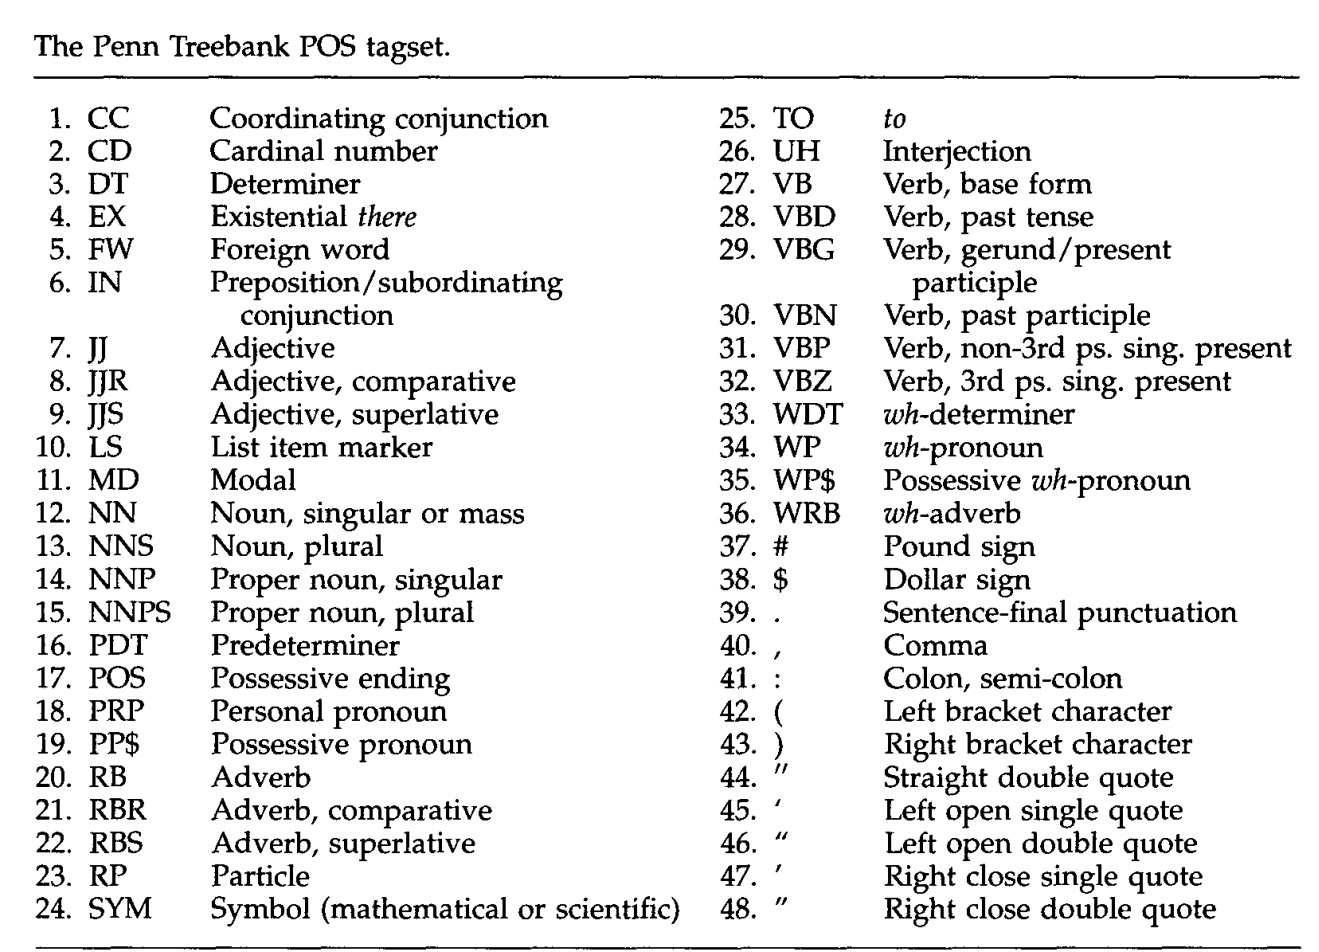
\includegraphics[scale=0.3]{graficos/penn-tagset}
  \caption{Tagset Penn Treebank}
  \label{fig:tagset-penn}
\end{figure}

Por su parte, el POS-tagger español de Freeling, por su naturaleza multilingüe, utiliza el tagset propuesto por el grupo EAGLES (\textit{Expert Advisory Group on Language Engineering Standards})\footnote{\url{http://www.ilc.cnr.it/EAGLES96/home.html}}, una organización europea que fomenta la investigación de procesamiento de lenguajes multilingüe, mientras que por una cuestión de compatibilidad, se preservan los tags de Penn Treebank para el inglés. Los tags de EAGLES tienen en consideración diferentes matices para contemplar las variaciones de diferentes idiomas. Sobre un conjunto inicial de 12 categorías -las 9 recién enunciadas más \sq{Signos de puntuación}, \sq{Numerales} y \sq{Fechas y horas} define etiquetas mucho más especificas. En concreto, un tag consta de entre 6 y 7 atributos, cada uno de las cuales expresa una característica de la palabra dependiendo del valor especificado en el atributo anterior (salvo, claro, la primera posición, que especifica la clase general). Para algunas clases alguno de estos valores no tienen sentido, mientras que para algunas palabras algunos valores no están o no pueden definirse (en el caso de subespecificación de un atributo, esta se nota como un \sq{0}).
En las tablas \ref{tabla_2_4} y \ref{tabla_2_5} presentamos la especificación para el conjunto de tags relacionados con sustantivos y un ejemplo de su aplicación.

\begin{center}
\begin{table}
\centering
\begin{tabular}{| l | l | l | l |}
 \hline
 \multicolumn{4}{|c|}{Nombres} \\ \hline
Pos. & Atributo & Valor & Código \\ \hline
1 & Categoría &  Nombre & N \\ \hline
\multirow{2}{*}{2} & \multirow{2}{*}{Tipo} & Común  & C \\ \cline{3-4}
  & &      Propio & P \\ \hline
\multirow{3}{*}{3} & \multirow{3}{*}{Género} & Masculino & M \\ \cline{3-4}
 & & Femenino &  F \\ \cline{3-4}
 & & Común    & C  \\ \hline
\multirow{3}{*}{4} & \multirow{3}{*}{Número} & Singular & S \\ \cline{3-4}
 & & Plural &  P \\ \cline{3-4}
 & & Invariable & N  \\ \hline
 \multirow{4}{*}{5-6} & \multirow{4}{*}{Clasificación Semántica} & Persona & SP \\ \cline{3-4}
 & & Lugar &  G0 \\ \cline{3-4}
 & & Organización &  O0 \\ \cline{3-4}
 & & Otros & V0  \\ \hline
\multirow{2}{*}{7} & \multirow{2}{*}{Grado} & Aumentativo  & A \\ \cline{3-4}
  & & Diminutivo & D \\ \hline
\end{tabular}
\caption{Valores para cada coordenada de tags para sustantivos}
\label{tabla_2_4}
\end{table}
\end{center}


\begin{center}
\begin{table}
\centering
\begin{tabular}{| l | l | l |}
 \hline
Forma & Lema & Etiqueta \\ \hline
chico & chico & NCMS000 \\ \hline
chicas & chico & NCFP000 \\ \hline
gatito & gato & NCMS00D \\ \hline
oyente & oyente & NCCS000 \\ \hline
oyentes & oyente & NCCP000 \\ \hline
cortapapeles & cortapapeles &NCMN000 \\ \hline
tesis & tesis & NCFN000 \\ \hline
Barcelona & barcelona & NP000G0 \\ \hline
COI & coi & NP000O0 \\ \hline
Pedro & pedro & NP000P0 \\ \hline
\end{tabular}
\caption{Ejemplos de tags y lemas para sustantivos}
\label{tabla_2_5}
\end{table}
\end{center}


Existen varios enfoques algorítmicos al problema del POS tagging: desde los más primitivos basados en reglas escritas a mano pasando a los basados en HMMs (Hidden Markov Models), Maximum Entropy o Transformation Based Learning. Un detalle de estos métodos excede la introducción al problema que supone esta sección de la tesis. El POS tagger de Freeling está basado en el approach de HMMs y el de Stanford en el de Maximum Entropy, ambos modelos de machine learning. En \allref{subsec:freeling-pos} y \allref{sec:stanford-tools} se encuentran algunos comentarios más técnicos de los algoritmos de POS tagging que utilizamos en este trabajo y vínculos a bibliografía pertinente y en la sección siguiente \allref{subsec:nerc} veremos una descripción más detallada de enfoques algorítmicos a ese problema que ilustrará, al menos de modo general, la estructura de la algoritmia basada en machine learning aplicada a procesamiento de lenguajes.
En la tabla \ref{ejemplos_de_postagging} listamos ejemplos concretos de análisis de la oración de ejemplo del comienzo de esta sección (\dq{El hombre bajó la escalera.}) para mostrar un funcionamiento real de los algoritmos utilizados en esta tesis.


\begin{center}
\centering
\begin{table}
\begin{tabular}{| l | l | l |}
\hline
\multicolumn{3}{|c|}{Freeling (ES)} \\ \hline
Forma &  Etiqueta & Descripción \\ \hline
El & DA0MS0 & Determinante, Artículo, Masculino, Singular\\ \hline
hombre & NCMS000 & Nombre, Común, Masculino, Singular  \\ \hline
bajó & VMIS3S0 & Verbo, Principal, Indicativo, Pasado, Tercera Persona, Singular\\ \hline
la & DA0FS0 & Determinante, Artículo, Femenino, Singular\\ \hline
escalera& NCFS000 & Nombre, Común, Femenino, Singular \\ \hline
.& Fp& Punto final\\ \hline \hline
\multicolumn{3}{|c|}{Freeling (EN)} \\ \hline
Forma & Etiqueta & Descripción \\ \hline
The &DT & Determiner \\ \hline
man &NN & Noun, singular or mass \\ \hline
came  &VBD& Verb, past tense\\ \hline
down  &RP& Particle \\ \hline
the &DT& Determiner \\ \hline
stairs & NNS& Noun, plural \\ \hline
.& Fp& Sentence final punctuation \\ \hline \hline
\multicolumn{3}{|c|}{Stanford (EN)} \\ \hline
Forma & Etiqueta & Descripción \\ \hline
The &DT & Determiner \\ \hline
 man & NN & Noun, singular or mass \\ \hline
  came &VBD  & Verb, past tense \\ \hline
 down & RP  &  Particle\\ \hline
 the & DT  &  Determiner \\ \hline
 stairs. &NN   & Noun, plural \\ \hline
 \end{tabular}
\caption{Ejemplos de POS tagging}
\label{ejemplos_de_postagging}
\end{table}
\end{center}

En el scope de este proyecto, utilizamos pos-tagging para filtrar clases de palabras inútiles y para seleccionar tres tipos: las qwords, los verbos y los sustantivos (Las qwords son los pronombres interrogativos: qué, quién, cómo, etc. y en inglés, who, when, where...). \newline


\subsection{Reconocimiento de Entidades Nombradas (NER)}
\label{subsec:nerc}

El reconocimiento de entidades nombradas (NER, de Named Entity
Recognition) es una subtarea de Information Extraction. Information
Extraction es, brevemente, todo el dominio de problemas vinculado con
la extracción de información estructurada a partir de datos no
estructurados o semi estructurados. NER es, dentro de este dominio, el
proceso de reconocer unidades de información (las entidades
nombradas) tales como nombres de personas, organizaciones, lugares,
expresiones numéricas como tiempo, fechas, dinero, porcentajes, etc.
A veces se habla de NERC (Named Entity Recognition and Classification)
para poner énfasis en la asignación de un tipo (por ejemplo: nombre
de empresa) a la entidad nombrada reconocida.

Los primeros sistemas de NER eran algoritmos basados en reglas
hardcodeadas, mientras que los modernos incorporan técnicas de
machine learning y son, en general, algoritmos basados en features.

El primer sistema data de 1991 y constaba de reglas escritas a mano y
heurísticas simples. Recién en 1996, con el estímulo de la MUC-6
(una conferencia reconocida en el área que dedicó una edición a
NER), el área comenzó a acelerar su crecimiento.

Muchos trabajos sobre NER están basados sólo en inglés, pero también existen trabajos para otros idiomas y, más en general, que buscan la independencia del idioma (o también ser multi-idioma). En la CONLL-2003 (otra conferencia reconocida del área) se trabaja fuertemente el problema NER para el alemán, mientras que en la CONLL-2003 se estudia el español y el holandés y, en general, el estado de arte tiene avances, más o menos prometedores, para una gran variedad de idiomas.

El problema del reconocimiento de entidades nombradas está acotado a lo que el filósofo del lenguaje Saúl Kripke llamó “designador rígido”, dejando afuera las descripciones definidas. Por ejemplo, podemos referirnos a Saúl Kripke como “Saúl Kripke” o como “el filósofo de lenguaje que acuñó el concepto de designador rígido”. El primer ejemplo es un designador rígido y un NER debería detectarlo, mientras que el segundo es una descripción y por lo tanto queda afuera de esta subtarea. Notar que ambos denotan unívocamente a un individuo. Para identificar a la compañía automotriz creada por Henry Ford, dos designadores rígidos son “Ford” y “Ford Company”, etc. Más en general, los designadores rígidos incluyen nombres propios tanto como clases naturales (por ejemplo, especies de biología y nombres de sustancias, etc). Además, se incorpora al problema la detección de expresiones temporales (“26 de Agosto de 2013”) y ciertas expresiones numéricas como dinero (“U\$D 250”) y otros tipos de unidades (“20\%”, “10,25”, etc). En un principio se buscaba detectar nombres propios en general, pero luego se incorporó la clasificación como un paso de esta subtarea. Las clases más utilizadas, por una cuestión completamente pragmática, son: persona, organización y lugar (location). Estas tres clases se conocen con el nombre de ENAMEX. A su vez, existen trabajos que subclasifican estas tres clases, dando como output, para un lugar (location), un subtipo como  “ciudad”, “estado” o  “país” y para personas alguna definición más específica (“político”, “farandulero”, “deportista”, etc). Algunos trabajos incluyen otras clases como “varios”, para aquellos que no caen con un grado alto de confiabilidad en ninguna categoría, y también categorías específicas para los valores numéricos (date, time, money, percent, etc). Las categorías estándar pueden, sin embargo, adaptarse a las clases de entidades nombradas de un dominio de problemas puntual, pero por lo general este enfoque requiere del entrenamiento de módulos de machine learning, lo cual suele requerir una serie de inputs de los que no siempre se dispone (principalmente, un corpus de datos suficientemente grande para entrenar el sistema y la disponibilidad temporal para configurarlo).


Además de los ya mencionados sistemas de reconocimiento de entidades nombradas basados en reglas escritas a mano del comienzo de las investigaciones en el área, existen los basados en machine learning, en los cuales vamos a detenernos brevemente en esta sección. Los algoritmos basados en machine learning son entrenados sobre un corpus de datos con ejemplos positivos y negativos de entidades nombradas, a partir de los cuales infieren sus propias reglas de reconocimiento basadas en features. Hay tres tipos de enfoques al problema basados en machine learning: aprendizaje supervisado, aprendizaje semi supervisado y aprendizaje no supervisado.
El aprendizaje supervisado es la técnica actualmente más utilizada para resolver el problema de reconocimiento de entidades. Estos métodos incluyen Hidden Markov Models (HMM), Decision Trees, Maximum Entropy Models (ME), Support Vector Machines (SVM)  y Conditional Random Fields (CRF). Estos métodos son variantes de un modelo único de aprendizaje supervisado que consiste en leer un gran corpus de datos anotados, crear features de identificación y clasificación de entidades a partir de estos datos (generar un \textit{modelo entrenado}) y finalmente identificar y clasificar un input nuevo en base a este modelo.

En cuanto al aprendizaje semi supervisado, la principal técnica aplicada a NER es conocida como “bootstraping” e involucra un grado de supervisión bajo, como por ejemplo, configurar un conjunto inicial de semillas (seeds) para el algoritmo de aprendizaje. Más genéricamente, un algoritmo de aprendizaje semi automático podría buscar a partir de los ejemplos iniciales (dados manualmente) otras entidades que cumplan el mismo rol léxico en contextos similares, para luego iterar sobre el conjunto ampliado.
Otro enfoque consiste en aplicar una serie de reglas simples basadas en patrones (por ejemplo: “New York” es una entidad de tipo location; si empieza con “Sr.” es una entidad de tipo person”) y luego identificar contextos de uso común sobre un corpus para generar reglas basadas en contextos. Un contexto puede incluir desde el rol semántico de las palabras en cuestión hasta ciertos patrones (como por ejemplo “empezar con ‘Sr.’”).

Finalmente, existen algoritmos de reconocimiento de entidades basados en aprendizaje no supervisado. El enfoque típico es el clustering, por ejemplo: agrupar entidades nombradas de diferentes clusters basados en similaridad de contexto.  La forma general consiste en aplicar diferentes recursos léxicos (por ejemplo, Wordnet) sobre patrones léxicos y estadísticas tomadas de un gran corpus no anotado.

En nuestro trabajo utilizamos los NER taggers de Stanford\cite{NER2} y de Freeling, el primero implementando un algoritmo CRF, es decir, de aprendizaje supervisado (ver \allref{sec:stanford-tools}) mientras que el segundo es un algoritmo trivial basado en Autómatas Finitos (ver \allref{subsec:freeling-mods}). Para descripciones y referencias de diferentes implementaciones de algoritmos de NERC ver \cite{NER1}.


\subsection{Clasificación de Preguntas (QC)}
\label{subsec:qc}
Question Classification es la tarea de categorizar preguntas en diferentes
clases semánticas que impongan restricciones significativas a las respuestas potenciales
para utilizarlas en fases posteriores del proceso de QA.
La clasificación de preguntas es una subclase del problema de la clasificación.
Un clasificador es una herramienta que asigna a un elemento una de
\textit{k} clases. La clasificación es un área bastante fecunda de PLN y, más en general, de machine learning.
Los clasificadores de preguntas son herramientas que clasifican preguntas según su tipo de respuesta esperada. Por ejemplo:
\dq{?`Quién descubrió América?} espera, más allá del nombre concreto, \textit{un nombre de persona}; {\textquotedblleft}?`Cuándo se descubrió
América?{\textquotedblright} espera \textit{una fecha} (o, más en
general, \textit{un tiempo}), {\textquotedblleft}?`Dónde se
descubrió América?{\textquotedblright} espera, como respuesta,
\textit{un lugar}, etc. Este es un eje de clasificación conocido como
tipo de respuesta esperado, aunque existen otros. Notar que el último ejemplo, en concreto confuso (¿tiene sentido la pregunta?), no lo es a nivel estructural.

El rol del módulo de QC en un sistema de QA es doble: Por un lado, impone restricciones a la respuesta final, permitiendo filtrar y verificar respuestas candidatas.
Por otra lado, provee información para estructurar el flujo de código de los procesos subsiguientes, permitiendo implementar estrategias puntuales para cada tipo de respuesta esperada. Por ejemplo, para la pregunta \dq{?`Quién fue el primer presidente constitucional de Argentina?} resulta de gran utilidad, a la hora de evaluar pasajes, saber que la respuesta esperada debe ser una \textit{persona}: de este modo se puede evitar el procesamiento lingüístico de un gran dominio de pasajes no relevantes, por ejemplo, pasajes que no contienen ninguna entidad nombrada de tipo \dq{persona}. Estas mismas razones justifican la deseabilidad de la especificidad: saber que la respuesta final debe ser un \textit{presidente} o un \textit{político} es más informativo y útil para el resto del proceso que solo saber que es una \textit{persona}.

Debido a la complejidad de análisis lingüístico intrínseca en la clasificación específica, los sistemas de QC más básicos adoptan un esquema de clases acotado y basado en reglas simples. Típicamente, las clases son: \textit{Persona}, \textit{Lugar}, \textit{Organización}, \textit{Fecha}, \textit{Cantidad}, \textit{Duración} y \textit{Medida}, mientras las reglas de clasificación son parecidas a las siguientes:
\begin{itemize}
\item Si la pregunta empieza con \textit{Quién} o \textit{Quiénes}, entonces el tipo es \textit{Persona}
\item Si la pregunta empieza con \textit{Dónde}, entonces el tipo es \textit{Lugar}
\item Si la pregunta empieza con \textit{Cuándo}, entonces el tipo es \textit{Fecha}
\item Si la pregunta empieza con \textit{Qué}, entonces determinar el tipo de acuerdo al sustantivo principal de la pregunta (utilizando pos-tagging)
\item ...
\end{itemize}

Como nota al pie, este esquema de clasificación semántico es uno entre otros. Por ejemplo, \cite{QC-other} propuso un esquema \textit{conceptual} de 13 clases en las que incluye, por ejemplo: antecedentes y consecuencias causales, habilitación, verificación, disyunción, etc.

Estas reglas básicas -triviales, si se quiere- cubren gran parte de las preguntas con una eficacia alta. En \allref{sec:stanford-tools} presentamos un enfoque más complejo que permite una clasificación más granular, basado en machine learning. El uso de algoritmos de machine learning tiene una serie de ventajas interesantes a la hora de definir un sistema de clases complejo. Como mencionamos al hablar de los otros taggers, la definición de reglas manuales es una tarea tediosa y con poca capacidad de adaptarse o modificarse, mientras que la definición de un set de features adecuado para el aprendizaje programático, en cambio, permite la fácil incorporación de nuevas clases y/o la incorporación de nuevas mejoras descubiertas. Por otro lado, un esquema de clases semánticamente rico -más granular que el modelo básico recién enunciado- requiere la consideración de una gran cantidad de dimensiones lingüísticas, tanto sintácticas como semánticas, lo que hace que la definición manual de reglas una tarea potencialmente imposible en términos de costo de tiempo humano.

Finalmente, cabe mencionar que no existen clasificadores de preguntas para el español y que a la hora de abordar este problema en nuestra implementación debimos apelar a mecanismos ad-hoc.

\subsection{Otras tareas}
\label{subsec:otras-tareas-pnl}
Otras tareas de procesamiento de lenguajes que son parte de la \sq{caja de herramientas} con las que podemos encarar problemas que requieran análisis lingüísticos son: detección de idiomas, resolución de correferencias,\footnote{Por ejemplo: en \dq{Nietzsche murió en 1900. Antes de morir, él estuvo aquejado de una enfermedad mental degenerativa}, \textit{él} refiere a \textit{Nietzsche}.} generación de árboles sintácticos y de dependencias, codificación fonética, anotaciones basadas en recursos léxicos (como Wordnet), desambiguación de sentido de palabras (Word sense disambiguation), extracción de relaciones \footnote{Por ejemplo, para \dq{Nietzsche murió en 1900.} extraer la relación \textit{morir(Nietzsche, 1900)}.} y traducción automática (o machine translation).

Finalmente, la lematización y el stemming son dos tareas de uso frecuente también. La lematización consiste en agrupar diferentes formas de una palabra bajo un ítem único. Por ejemplo, el verbo en infinitivo \textit{caminar} puede aparecer bajo diferentes conjugaciones y formas: \textit{caminó, caminando, caminando, caminamos}, etc. Un lematizador tomaría como input alguna de estas formas y devolvería \textit{caminar}. La lematización es un proceso similar al stemming, con la diferencia de que el stemming opera sobre una sola palabra, sin información del contexto de ocurrencia (las palabras que la rodean en el contexo de emisión) y, en consecuencia, pierde información útil (como el pos tag, para el que se requiere el contexto), siendo algoritmos más simples y eficientes, pero menos precisos que la lematización.
\chapter{Estado de Arte}
\label{chap:estado-de-arte}
En esta secci\'on vamos a pasar revista de una serie de tecnolog\'ias
investigadas o testeadas durante la tesis. La primera, IBM-Watson es
quiz\'as la m\'as conocida para el p\'ublico en general. 


//write stuff\newline


\section{IBM-Watson}

Watson es un sistema dise\~nado por IBM con el objetivo de competir en
tiempo real en el programa de televisi\'on estadounidense Jeopardy,
logrando resultados del nivel de los campeones humanos de este
programa.

El proyecto demor\'o 3 a\~nos de investigaci\'on, en los cuales se
logr\'o obtener la performance esperada (nivel humano experto) en
cuanto a precisi\'on, confiabilidad y velocidad, logrando derrotar a
dos de los hombre con mayores r\'ecords hist\'oricos del show en un
programa en vivo [M\'AS DATOS -LINKS]

El objetivo del \ proyecto puede considerarse una extensi\'on de lo que
fue Deep Blue, el sistema que logr\'o el nivel de los expertos humanos
en el ajedrez, porque busc\'o superar un reto que significativo y
visible del campo de la Inteligencia Artificial tanto para la comunidad
cient\'ifica como para la sociedad en general:
{\textquotedblleft}?`puede un sistema computacional ser dise\~nado para
competir con los mejores hombre en alguna tarea que requiera altos
niveles de inteligencia humana y, si es el caso, que clase de
tecnolog\'ia, algoritmos e ingenieria se
requiere?{\textquotedblright}\footnote{\ Traducci\'on propia de
Building Watson: An Overview of the DeepQA Project, p2}

Watson es la implementaci\'on espec\'ifica para participar en este
programa de una arquitectura m\'as gen\'erica de question answering,
DeepQA, que da el nombre al proyecto de la corporaci\'on. Esta
arquitectura ejemplifica perfectamente la complejidad del problema de
QA de dominio abierto e incorpora tecnolog\'ias de punta de distintos
dominios de ciencias de la computaci\'on, y de IA en particular:
information retrieval, natural language processing, knowledge
representation and reasoning, machine learning e interfaces humano -
computadora.

\subsection{El problema}

Watson debe realizar tareas como parsing, question classification,
question descomposition, automatic source adquisition and evaluation,
entity and relation detection, logical form generation, knowledge
representation and reasoning manteniendo ciertos atributos de calidad
bastante exigentes derivados de la naturaleza del show. Estas
restricciones son:

\begin{itemize}
\item Confiabilidad de la respuesta: \newline
Jeopardy tiene tres participantes con un pulsador y el que desee
responder debe pulsar antes que los dem\'as. Adem\'as, existe una
penalizaci\'on por respuestas incorrectas, por lo que es esencial que
el sistema pueda determinar la confiabilidad de la respuesta obtenida a
fin de optar por responder o no responder.
\item Tiempos de respuesta: \newline
La confiabilidad de la respuesta, o al menos una estimaci\'on, debe
calcularse antes de que pase el tiempo para decidir responder (6
segundos) y tambi\'en de que otro participante oprima su pulsador
(menos de 3 segundos).
\item Precisi\'on:\newline
El tipo de respuestas que se dan en el show suelen ser respuestas
exactas (por ejemplo: solamente un nombre, un n\'umero o una fecha,
etc). 
\end{itemize}

\bigskip

El sistema cuenta con varios componentes heur\'isticos que estiman
ciertos features y grados de confiabilidad para diferentes respuestas,
los cuales son evaluados por un sistema general que sintetiza un grado
de confiabilidad para una respuesta final y determina as\'i si
responder o no responder. 

El programa consta de un tablero con 30 pistas (o preguntas) organizadas
en seis columnas, cada una de las cuales es una categor\'ia. Las
categor\'ias van desde temas acotados como
{\textquotedblleft}historia{\textquotedblright} o
{\textquotedblleft}ciencias{\textquotedblright} hasta temas m\'as
amplios como {\textquotedblleft}cualquier cosa{\textquotedblright} o
{\textquotedblleft}potpourri{\textquotedblright}. Watson intenta
respuestas sobre varias hip\'otesis de dominio y verifica en cual de
ellos se logran respuestas de mayor confiabilidad. 

Por otra parte, el grueso de las preguntas de Jeopardy son del tipo
\textit{factoid}, esto es, preguntas cuya respuesta esta basada en
informaci\'on f\'actica acerca de una o m\'as entidades individuales.


\bigskip

Por ejemplo:

Categor\'ia: Ciencia General

Pista: Cuando es impactado por electrones, un f\'osforo emite energ\'ia
electromagn\'etica de esta forma

Respuesta: Luz (o fotones)


\bigskip

A su vez, existen ciertos tipos de pistas que requieren un enfoque
particular, por ejemplo, pistos que constan de dos subpistas muy
d\'ebilmente relacionadas, o problemas matem\'aticos formulados en
lenguaje humano, o problemas de fon\'etica, etc, que no pueden ser
simplemente dejados de lado porque, si bien tiene poca probabilidad de
aparici\'on, cuando aparecen lo hacen en bloque y pueden arruinar el
juego de Watson. Se acord\'o con la productora del programa, sin
embargo, dejar de lado preguntas audiovisuales (aquellas que presentan
una imagen o un audio y requieren interpretarlo) y preguntas que
requieren instrucciones verbales del presentador.


\bigskip

Para determinar el dominio de conocimiento, los investigadores
analizaron 20000 preguntas, extrayendo su LAT (lexical answer type, o
tipo l\'exico de respuesta). El LAT se define como una palabra en la
pista que indica el tipo de la respuesta esperado. Por ejemplo, para la
pista {\textquotedblleft}Investanda en 1500{\textquoteright}s para
agilizar el juego, este movimiento involucra dos
piezas{\textquotedblright} el LAT es
{\textquotedblleft}movimiento{\textquotedblright}. Menos del 12\% de
las pistas no indicaba expl\'icitamente ning\'un LAT, usando palabras
como {\textquotedblleft}esto{\textquotedblright} o
{\textquotedblleft}eso{\textquotedblright}. En estos casos, el sistema
debe inferir el tipo de respuesta del contexto. Del an\'alisis de estas
20000 pistas se reconocieron 2500 tipos l\'exicos distintos, de los
cuales los 200 m\'as frecuentes no llegaban a cubrir el 50\% del total
de pistas. Esto implica que un approach estructurado (orientado por el
tipo de respuesta), si bien resulta \'util para algunos tipos, no es
suficiente para abordar el problema completo.

\subsection{M\'etricas}

Las m\'etricas de resultados, adem\'as del tiempo de respuesta, son la
\textit{precisi\'on} (preguntas contestadas correctamente / preguntas
contestadas) y el \textit{porcentaje de respuestas dadas }(preguntas
contestadas / total de preguntas). Mediante la configuraci\'on de un
threshold de \textit{confiabilidad} pueden obtenerse distintas
estrategias de juego: un umbral bajo repercutir\'a en un juego m\'as
agresivo, incrementando la proporci\'on de respuestas contestadas,,
pero disminuyendo su precisi\'on, mientras que un umbral alto
determinar\'a un juego conservador, con menos respuestas dadas pero
mayor precisi\'on en las mismas. Es un cl\'asico escenario de trade-off
entre dos atributos de calidad. Un buen sistema de estimaci\'on de
confiabilidad implica una mejora general del sistema, a\'un cuando el
m\'odulo de generaci\'on de respuestas permanezca id\'entico.


\bigskip

En el show, el porcentaje de respuestas dadas depende de la velocidad
con la que se llega a presionar el pulsador, lo cual s\'olo interesa
para el dominio de QA como una restricci\'on temporal. 


\bigskip

Mediante an\'alisis num\'erico, los investigadores determinaron que los
campeones de Jeopardy lograban tomar entre el 40\% y el 50\% de las
preguntas y, sobre ellas, lograban una precisi\'on de entre el 85\% y
el 95\%, lo que determinaba una barrera de performance bastante
exigente en lo que respecta a QA.


\bigskip

\subsection{Baseline}

El equipo de IBM intent\'o utilizar dos sistemas consolidados en QA y
adaptarlos al problema \ de Jeopardy. \ El primero fue PIQUANT
(Practical Intelligent Question Answering Technology), un sistema
desarrollado por IBM en conjunto con el programa del gobierno
estadounidense AQUAINT y varias universidades, que estaba entre los
mejores seg\'un la TREC (Text Retrieval Conference), una autoridad en
el \'area. PIQUANT consta de un pipeline t\'ipico (v\'ease QANUS) con
tecnolog\'ia de punta, logrando un rango del 33\% de respuestas
correctas en las evaluaciones TREC-QA. Los requerimientos de la
evaluaci\'on de TREC son muy distintos de los de Jeopardy: TREC ofrece
un corpus de conocimiento relativamente peque\~no (1M de documentos) de
donde las respuestas deben ser extra\'idas y justificadas, el tipo de
preguntas de TREC son menos complejas a nivel ling\"u\'istico que las
de Jeopardy y la estimaci\'on de confiabilidad no resulta una m\'etrica
importante (dado que no hay penalizaci\'on por respuestas incorrectas).
Adem\'as, los sistemas tienen permitido acceder a la web y las
restricciones temporales son, por mucho, m\'as amplias (por ejemplo:
una semana para responder 500 preguntas). En Jeopardy, adem\'as de las
restricciones ya mencionadas, un requerimiento fue que el sistema
trabaje sobre datos locales y no acceda a la web en tiempo real. El
intento de adaptar PIQUANT al problema de Jeopardy dio p\'esimos en
comparaci\'on con los necesarios: 47\% de precisi\'on sobre el 5\% de
respuestas con mayor confiabilidad y 13\% de precisi\'on en general. 

Por otro lado, el equipo intent\'o adaptar el sistema OpenEphyra
(v\'ease OpenEphyra), un framework open-source de QA desarrollado en
CMU (Carnegie Mellon University) basado en Ephyra (no libre),
dise\~nado tambi\'en para la evaluaci\'on TREC. OpenEphyra logra un
45\% de respuestas correctas sobre el set de datos de evaluaci\'on TREC
2002, usando busqueda web. La adaptaci\'on result\'o a\'un peor que la
de PIQUANT (con menos del 15\% de respuestas correctas y una mala
estimaci\'on de la confiabilidad). 

Se probaron dos adaptaciones de estos sistemas. una basada en
b\'usquedas de texto puro y otra basada en reconocimiento de entidades.
En la primera, la base de conocimiento se model\'o de manera no
estructurada y las preguntas se interpretaron como t\'erminos de una
query, mientras que en la segunda se model\'o una base de conocimientos
estructurada y las preguntas se analizaron sem\'anticamente para
reconocer entidades y relaciones, para luego buscarlos en la base.
Comparando ambos enfoques en base al porcentaje de respuestas dadas, el
primero dio mejores resultados para el 100\% de las respuestas,
mientras que la confiabilidad general era baja; por otro lado, el
segundo enfoque logr\'o altos valores de confiabilidad, pero s\'olo en
los casos en que efectivamente logra identificar entidades. De aqu\'i
se infiere que cada enfoque tiene sus ventajas, en el dominio de
problemas apropiado.

\subsection{La arquitectura DeepQA}
\label{subsec:deep-qa}
Los intentos de adaptaci\'on iniciales, como vimos, no dieron
resultados, as\'i como tampoco sirvieron las adaptaciones de algoritmos
de la literatura cient\'ifica, los cuales son realmente dif\'iciles de
sacar de su contexto original y de las evaluaciones sobre las cuales
fueron testeados. Este problema, veremos -por ejemplo, con QANUS y
Reverb- , se repiti\'o en nuestro proyecto. Como conclusi\'on de estos
intentos frustrados, el equipo de IBM entendi\'o que una arquitectura
de QA no deb\'ia basarse en sus componentes concretos sino en la
facilidad para incorporar nuevos componentes y para adaptarse a nuevos
contextos. As\'i surgi\'o DeepQA, la arquitectura de base, de la cual
Watson es una instancia concreta para un contexto particular (con
requerimientos de alta precisi\'on, buena estimaci\'on de
confiabilidad, lenguaje complejo, amplitud de dominio y restricciones
de velocidad). DeepQA es una arquitectura de computo paralelo,
probabilistico, basado en recopilaci\'on de evidencia y scoring. Para
Jeopardy se utilizaron m\'as de 100 t\'ecnicas diferentes para analizar
lenguaje natural, identificar y adjudicar valor a fuentes de
informaci\'on, encontrar y generar hip\'otesis, encontrar y rankear
evidencias y mergear y rankear hip\'otesis en funci\'on de esta
evidencia. La arquitectura sirvi\'o para ganar Jeopardy, pero tambi\'en
se adapt\'o a otros contextos como la evaluaci\'on TREC, dando
resultados mucho mejores que sus predecesores. Los principios de
dise\~no subyacentes de la arquitectura son:

\begin{itemize}
\item Paralelismo masivo\newline
Para evaluar distintas hip\'otesis en distintos dominios con poco
acoplamiento.
\item Pervasive confidence estimation:\newline
Ning\'un componente genera la respuesta final, sino que da una serie de
features y grados de confiabilidad y evidencia para distintas
hip\'otesis, que luego son sintetizados.
\item Integrate shallow and deep knowledge:
\end{itemize}

\bigskip

A continuaci\'on, enumeraremos la lista de pasos que sigue el sistema
para obtener la respuesta a una pregunta:

\subsubsection{Adquisici\'on de contenidos}

El primer paso de DeepQA es la adquisici\'on de contenidos. Este paso es
el \'unico que no se realiza en tiempo de ejecuci\'on y consiste en
crear la base de conocimiento en la cual el proceso final buscar\'a la
respuesta a la pregunta, combinando subprocesos manuales y
autom\'aticos. 

En principio se caracteriza el tipo de preguntas a responder y el
dominio de aplicaci\'on. El an\'alisis de tipos de preguntas es una
tarea manual, mientras que la determinaci\'on del dominio puede
encararse computacionalmente, por ejemplo, con la detecci\'on de LATs
que se\~nalamos antes. Dado el amplio dominio de conocimientos que
requiere Jeopardy, Watson cuenta con una gran cantidad de
enciclopedias, diccionarios, tesauros, art\'iculos acad\'emicos y de
literatura, etc. A partir de este corpus inicial, el sistema busca en
la web documentos relevantes y los relaciona con los documentos ya
presentes en el corpus. 

Adem\'as de este corpus de documentos no estructurados, DeepQA maneja
contenidos semi-estructurados \ y estructurados, incorporando bases de
datos, taxonom\'ias y ontolog\'ias como dbPedia, Wordnet y las
ontolog\'ias de Yago. 

\subsubsection{An\'alisis de la pregunta}

El primer paso en run-time es el an\'alisis de la pregunta. En este paso
el sistema intenta entender qu\'e es lo que la pregunta est\'a
preguntado y realizar los primeros an\'alisis que determinan c\'omo
encarar\'a el procesamiento el resto del sistema. Watson utiliza
shallow parses, deep parses, formas l\'ogicas, pos-tags,
correferencias, detecci\'on de entidades nombradas y de relaciones,
question classification, adem\'as de ciertos an\'alisis concretos del
domiento del problema.

En este proceso se clasifica el tipo de la pregunta (los tipos est\'an
determinados por el show: puzzles, matem\'aticos, etc). Tambi\'en se
busca el tipo de respuesta esperada, d\'onde los tipos manejados son
por Watson son los LATs extra\'idos de las preguntas de ejemplo. El LAT
determina el {\textquotedblleft}tipo{\textquotedblright} de la
respuesta, que clase de entidad \textit{es} la respuesta (una fecha, un
hombre, una relaci\'on, etc). El equipo de IBM intent\'o adaptar
distintos algoritmos de clasificaci\'on preexistentes, pero despu\'es
de intentar entrenarlos para el dominio de tipos de Jeopardy, llegaron
a la conclusi\'on de que su eficacia era dependiente del su sistema de
tipos default, y que la mejor forma de adaptaci\'on era mappear su
output a los tipos utilizados por Watson (un enfoque similar fue
utilizado en esta tesis con respecto al clasificador de Stanford). Otra
anotaci\'on importante es el
{\textquotedblleft}foco{\textquotedblright} de la pregunta, la parte de
la pregunta tal que si se la reemplaza por la respuesta, la pregunta se
convierte en una afirmaci\'on cerrada.

Por ejemplo, para {\textquotedblleft}El hombre que escribi\'o Romeo y
Julieta{\textquotedblright}, el foco es {\textquotedblleft}El hombre
que{\textquotedblright}. Este fragmento suele contener informaci\'on
importante sobre la respuesta y al reemplazarlo por una respuesta
candidata se obtiene una afirmaci\'on f\'actica que puede servir para
evaluar distintos candidatos y recolectar evidencia. Por ejemplo,
reemplazando por distintos autores y verificando que la oraci\'on
resultante est\'e presente en el corpus.

Por otro lado, muchas preguntas involucran relaciones entre entidades y,
m\'as puntualmente, tienen una forma sujeto-verbo-objeto. Por ejemplo,
tomando la pista anterior, podemos extraer la relaci\'on
\textit{escribir(x, Romeo y Julieta)}. La amplitud del dominio de
Jeopardy hace que la cantidad de entidad y de relaciones entre
entidades sea enorme, pero esto empeora a\'un m\'as al considerar las
distintas formas de expresar la misma relaci\'on. Por eso, Watson
s\'olo logra encontrar directamente una respuesta mediante
reconocimiento de entidades y relaciones sobre el 2\% de las pistas. En
general, este tipo de enfoque es \'util sobre dominios m\'as acotados,
mientras que la detecci\'on de relaciones como approach general a un
problema de question answering de dominio amplio es un \'area de
investigaci\'on abierta. 

Una particularidad ya se\~nalada de las preguntas de Jeopardy son las
pistas con subpistas no relacionadas. Para atacar este problema, Watson
genera distintas particiones y resuelve todas en paralelo, sintetizando
las respuesta de cada partici\'on generada mediante algoritmos ad-hoc
de ponderaci\'on de confiabilidad y otras caracter\'isticas.

\subsubsection{Generaci\'on de hipótesis}

El tercer paso (segundo en run-time) es la generaci\'on de hip\'otesis:
tomando como input el resultado del paso anterior se generan respuestas
candidatas a partir de la base de conocimiento offline. Cada respuesta
candidata reemplazada por el foco de la pregunta es considerada una
hip\'otesis, que el sistema luego verificar\'a buscando evidencias y
adjudicando un cierto grado de confiabilidad.

En la b\'usqueda primaria de respuestas candidatas, se busca generar
tantos pasajes como sea posible. El resultado final obtenido revela que
el 85\% de las veces, la respuesta final se encuentra entre los
primeros 250 pasajes devueltos por la b\'usqueda primaria. La
implementaci\'on utiliza una serie variada de t\'ecnicas, que incluyen
diferentes motores de b\'usqueda de textos (como Indri y Lucene),
b\'usqueda de documentos y de pasajes, b\'usquedas en bases de
conocimiento estructuradas como SPARQL con triple store y la
generaci\'on de mutiples queries a partir de una sola pregunta. La
b\'usqueda estructurada de triple stores depende del reconocimiento de
entidades y relaciones del paso anterior.

Para un n\'umero peque\~no de LATs, se defini\'o una suerte de conjunto
de entidades fijas (por ejemplo: pa\'ises, presidentes, etc). Si la
respuesta final no es retornada en este paso, entonces no hay
posibilidad de obtenerla en los siguiente. Por eso se prioriza el
recall sobre la precisi\'on, con el supuesto de que el resto del
pipeline lograr\'a filtrar la respuesta correcta correctamente. Watson
genera varios cientos de hip\'otesis candidatas en este paso.


\bigskip

\subsubsection*{(Soft filtering)}

Para optimizar recursos, se realiza un filtrado liviano de respuestas
antes de pasar a la recopilaci\'on de evidencia y al scoring de
hip\'otesis. Un filtrado liviano es, por ejemplo, comprobar similaridad
de la respuesta candidata con el LAT esperado de la respuesta. Aquellas
hip\'otesis que pasan el filtro pasan al siguiente proceso, que realiza
un an\'alisis m\'as exhaustivo.


\bigskip

\subsubsection{Recuperaci\'on de evidencias y scoring de pasajes}

Para recuperar evidencias se utilizan varios algoritmos. Uno
particularmente \'util es buscar la hip\'otesis candidata junto con las
queries generadas por la pregunta original, lo que se\~nala el uso de
la respuesta en el contexto de la pregunta. \ Las hip\'otesis con sus
evidencias pasan al siguiente paso, d\'onde se les adjudica un score. 

El proceso de scoring es donde se realiza la mayor parte del an\'alisis
m\'as fuerte a nivel computacional. DeepQA permite la incorporaci\'on
de distintos Scorers, que consideran diferentes dimensiones en las
cuales la hip\'otesis sirve como respuesta a la pregunta original. Esto
se llev\'o a cabo definiendo una interfaz com\'un para los scorers.
Watson incorpora m\'as de 50 componentes que producen valores y
diferentes features basados en las evidencias, para los distintos tipos
de datos disponibles (no estructurados, semi estructurados y
estructurados). Los scorers toman en cuenta cuestiones como el grado de
similaridad entre la estrurctura de la respuesta y de la pregunta,
relaciones geoespaciales y temporales, clasificaci\'on taxon\'omica,
roles l\'exicos y sem\'anticos que se sabe que el candidato puede
cumplir, correlaciones entre terminos con la pregunta, popularidad (u
obscuridad) de la fuente del pasaje, aliases, etc.

POR EJEMPLO: COPIAR NIXON

Los distintos scores se combinan luego en un score \'unico para cada
dimensi\'on.

(Merge)

Reci\'en despu\'es de este momento, Watson realiza un merge entre
hip\'otesis id\'enticas. Las hip\'otesis id\'enticas son diferentes
formulaciones ling\"uisticas de lo mismo, por ejemplo:
{\textquotedblleft}X naci\'o en 1928{\textquotedblright} o
{\textquotedblleft}El a\~no de nacimiento de X es
1928{\textquotedblright}. Finalmente, se procede a estimar un ranking
\'unico y una confiabilidad \'unica para las distintas hip\'otesis. En
este paso se utilizan t\'ecnicas de machine learning que requieren
entrenamiento, y modelos basados en scores. Se utilizan t\'ecnicas
jer\'arquicas como mixture of experts y stacked generalization y,
finalmente, un metalearner fue entrenado para ensamblar los distintos
resultados intermedios. 


\bigskip

\subsection{Tiempos y escala}

DeepQA utiliza Apache UIMA, un framework que implementa UIMA
(Unestructured Information Management Architecture): todos los
componentes de DeepQA son IUMA-annotators, m\'odulos que producen
anotaciones y aserciones sobre un texto.

La implementaci\'on inicial de Watson corr\'ia sobre un s\'olo
procesador y demoraba aproximadamente 2 horas en contestar una sola
pregunta. La arquitectura paralela permite, sin embargo, que al
correrlo sobre 2500 n\'ucleos -de la implementaci\'on final- los
tiempos de respuesta oscilen entre 3 y 5 segundos, que es lo esperado.

Finalmente, la implementaci\'on de Watson logr\'o alcanzar el est\'andar
de resultados de los campeones de Jeopardy y, como ya dijimos,
compiti\'o y gan\'o el programa en Febrero de 2011. Adem\'as, se
realizaron adaptaciones para trabajar sobre los problemas de TREC, en
los cuales se demostr\'o una amplia mejor\'ia en comparaci\'on con
PIQUANT y OpenEphyra


\bigskip

\subsection{Conclusiones sobre IBM-Watson}

System level approach.


\bigskip

\section{La arquitectura de Qanus}

QANUS (Question-Answering @ National University of Singapore) es un
sistema de question answering basado en information retrieval. El
proyecto se actualiz\'o por \'ultima vez en noviembre de 2012 y
contiene las herramientas m\'as actuales de nlp (el POS-tagger, el
NER-tagger y el Question Classifier de Stanford) y tambi\'en de
information retrieval \'indice de b\'usquedas lucene), todo de c\'odigo
abierto. El c\'odigo cuenta con un framework (Qanus), que cumple un rol
equivalente a la arquitectura DeepQA en el proyecto anterior, y un
sistema montado sobre este framework QA-sys, equivalente a Watson (Ver Figura ~\ref{fig:Quanus}). La
motivaci\'on de esto es proveer a la comunidad cient\'ifica un
framework para ingresar al mundo de QA de una manera m\'as sencilla y
r\'apida, permitiendo construir nuevos sistemas de QA sobre esta
arquitectura. En efecto, la arquitectura DeepQA no est\'a disponible
para la comunidad, el ya mencionado OpenEphyra, como veremos en breve,
no funciona, mientras que otros sistemas resultan igualmente
inaccesibles (Aranea, Qanda) mientras que QA-sys es un sistema de QA
out of the box. Mencionaremos los logros y los l\'imites de estos
objetivos cuando hablemos de nuestro intento por montar nuestro propio
sistema sobre Qanus. 

\begin{figure}
  \centering
    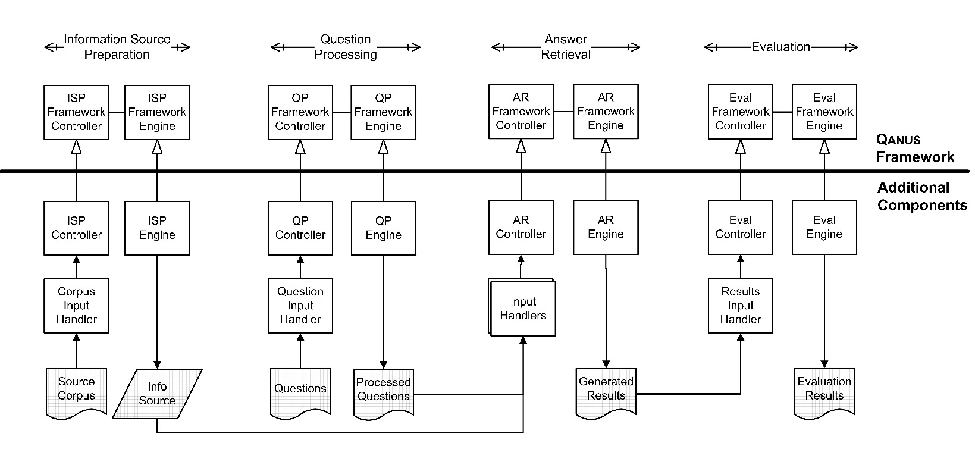
\includegraphics{graficos/Quanus}
  \caption{El framework Quanus y la implementación QA-sys}
  \label{fig:Quanus}
\end{figure}


La arquitectura, al igual que la de DeepQA, es la de un pipeline. Este
sistema consta de tres pasos principales, que se ejecutan todos por
separado (off-line): 


\bigskip

\subsection{Preparación de la fuente de información}
Este paso est\'a pensado para preprocesar cualquier base de conocimiento
y dejarla preparada para el paso 3 (retorno de la pregunta). El
framework se propone tan amplio que no hay m\'as especificaciones al
respecto. La implementaci\'on puntual asume una base de conocimiento en
formato XML de AQUAINT\footnote{\ } y la incorpora a un \'indice de
b\'usquedas Lucene. Este paso incorpora todo el conocimiento que
estar\'a finalmente offline; accesos din\'amicos a la web, por ejemplo,
se modelan en el paso 3.


\bigskip

\subsection{Análisis de la pregunta}
Este paso, igualmente gen\'erico, permite la incorporaci\'on de
distintos componentes para anotar los tokens de la pregunta con datos
\'utiles para ser consumidos por el paso 3. Otro procesamiento a
realizar en este paso podr\'ia ser la generaci\'on de queries
entendibles por los distintos motores de almacenamientos de
informaci\'on del paso 1. En particular, la implementaci\'on trae un
pos-tagger, un ner-tagger y un question classiffier, todos de Stanford.
Hablaremos m\'as de estos componentes m\'as adelante. 


\bigskip

\subsection{Generación de respuestas}
En este paso se utiliza la informaci\'on generada en la preparaci\'on
de la base de informaci\'on y en el procesamiento de la pregunta para
generar una respuesta. Tambi\'en puede incorporarse accesos a la web y
validaciones de las respuestas candidatas. La implementaci\'on concreta
eval\'ua cada pasaje de los primeros n documentos retornados por Lucene
para la pregunta original con una serie de componentes ad-hoc de
distancia para adjudicar diferentes grados de confiabilidad a los
distintos pasajes. \newline


Adem\'as, se provee de un cuarto paso opcional (el sistema de QA est\'a
completo con los tres pasos anteriores), para la fase de desarrollo y
de evaluaci\'on de la performance del sistema:\newline


\subsection{Evaluación}

Este paso est\'a pensado para evaluar las respuestas generadas y
presentarlas de un modo conciso en la fase de desarrollo.
B\'asicamente, cruza las respuestas obtenidas contra unas respuestas
esperadas escritas a mano y presenta el total de respuestas dadas
correctamente.


\bigskip

\subsection{Implementaci\'on}

El c\'odigo est\'a escrito en java y mantiene una interfaz com\'un a
todos los pasos: un controller cuyas responsabilidades son cargar los
componentes y un engine que utiliza los componentes para leer el input,
procesarlo y grabar el resultado. La adaptabilidad del framework est\'a
dada en la posibilidad de incorporar componentes respetando la interfaz
especificada para los mismos o bien, en modificar esta misma interfaz.
Presuntamente, el framework es lo suficientemente abierto para permitir
la implementaci\'on de sistemas basados en distintas fuentes de
conocimiento (ontolog\'ias, archivos, web) y con distintos modos de
funcionamiento mediante poco esfuerzo de customizaci\'on.

La implementaci\'on llamada QA-sys est\'a desarrollada para correr sobre
el tipo de datos de las evaluaciones TREC 2007 (XML AQUAINT). En el
primer paso, incorpora los XML en este formato a un \'indice Lucene, en
el segundo paso utiliza anota la pregunta con POS tags, NERs y
clasifica el tipo de respuesta con un clasificador entrenado y luego,
en el tercer paso se busca la pregunta sobre el \'indice lucene y se
retorna una lista con n documentos rankeados. Estos documentos se
subdividen en pasajes. Luego se aplican diferente algoritmos ad-hoc
dependiendo del tipo de respuesta esperada. \ Por ejemplo, si la
respuesta es un nombre de persona, se ejecuta NER sobre los diferentes
pasajes buscando nombres candidatos, si el tipo esperado es una fecha,
se utilizan expresiones regulares escritas a mano, etc. Finalmente, los
pasajes candidatos se eval\'uan utilizando heur\'isticas de proximidad
de los candidatos a la pregunta inicial. Para esto se utilizan
diferentes Scorers que rankean los pasajes seg\'un diferentes
caracter\'isticas (features) y luego se selecciona alguna priorizando
algunas caracter\'isticas sobre otras, dependiendo tambi\'en del tipo
de respuesta esperada. Por \'ultimo, el evaluador de resultados mide la
exactitud (\textit{accuracy}): total de respuestas correctas sobre
total de preguntas. QA-sys funciona s\'olo sobre preguntas del tipo
factoid y, a modo de comparaci\'on, el mejor sistema seg\'un la TREC
2007, el LymbaPA07 obtuvo un grado de exactitud del 0.706 y el d\'ecimo
(Quanta) obtuvo 0.206, mientras que QA-sys logra el 0.119. La
implementaci\'on es realmente simple y funciona s\'olo a modo de
ilustraci\'on de lo que puede construirse sobre el framework. 

\bigskip

\section{Otros sistemas de QA: OpenEphyra, Aranea y Just.Ask}

\bigskip

El paper describe las arquitecturas de todos los sistemas, si sirve
meter m\'as info

El paper [EPHYRA1] \ busca crear un criterio cuantitativo para comparar
la eficacia de distintos pasos de Just.Ask, Open Ephyra y Aranea
bas\'andose en la arquitectura \textit{pipeline de tres pasos}
compartida por todos. Los tres sistemas, por lo dem\'as, est\'an
basados en la web, utilizando distintas APIs de buscadores o bien
analizando los resultados de la interfaz de usuario de los mismos. 

El primer \'item importante a destacar de este trabajo, es que, al
momento de la experimentaci\'on \textbf{Aranea no funcionaba m\'as y
estaba discontinuado}\footnote{\ (Resaltado en Secci\'on 8, muy
concluyente).\par }\textbf{. }El autor se comunic\'o con el responsable
del proyecto que corrobor\'o que las APIs de los buscadores en los que
se basaba Aranea cambiaron y no hab\'ia inter\'es en readaptar el
c\'odigo para que vuelva a funcionar. Las comparaciones que logr\'o
entre Just.Ask y Open Ephyra son interesantes y concluyentes a favor de
la performance de OpenEphyra. 

(Freeling \ + Cambio de Base + Rigidez)

\chapter{Implementación de datos estructurados}
\label{chap:4}
En este capítulo, finalmente, nos toca hablar del primero de los dos sistemas implementados en este trabajo.
El sistema en cuestión implementa, con algunas limitaciones que mencionaremos, el modelo de Popescu descripto en \cite{QADB1} y \cite{QADB2} y reseñados por nosotros en \ref{subsec:closed-domain}.

Nuestro código está accesible públicamente en la siguiente dirección: \url{http://github.com/julian3833/popescu-world}. Allí pueden encontrarse, además del código en sí mismo, los procedimientos de instalación, ejemplos de ejecución y una lista con los principales puntos técnicos que pueden mejorarse (ver, también, \allref{subsec:popescu-cierre}).

Testeamos este sistema sobre la base de datos World, en inglés, ofrecida por MySQL\footnote{Ver \url{http://dev.mysql.com/doc/world-setup/en/index.html} y \url{http://dev.mysql.com/doc/index-other.html}} que consta de información geográfica básica sobre países, ciudades e idiomas.

Cabe mencionar que el scope original de este sistema era ser bilingüe y ejecutarse sobre una base de datos sobre universidades, empresas e investigación nacional del ámbito de la informática. Lamentablemente, por una cuestión de tiempos y de errores a la hora de estimar esfuerzos, no pudimos completar este plan original.

La estructura del capítulo es como sigue: En \ref{sec:popescu-db} pasamos revista de la base de datos que utilizamos para implementar el sistema y en \ref{sec:popescu-implementacion} discutimos la implementación. \ref{sec:popescu-implementacion} se divide, a su vez, en \ref{subsec:popescu-codigo}, donde discutimos la implementación en sí misma, \ref{subsec:popescu-ejemplos}, donde mostramos y comentamos algunos ejemplos de ejecuciones y \ref{subsec:popescu-cierre} donde analizamos los alcances, los límites y el trabajo futuro.


\section{Base de datos}
\label{sec:popescu-db}

La base de datos World consta de 3 tablas: Country, City y CountryLanguage (ver Figura \ref{fig:world-db}).

\begin{figure}
  \centering
    %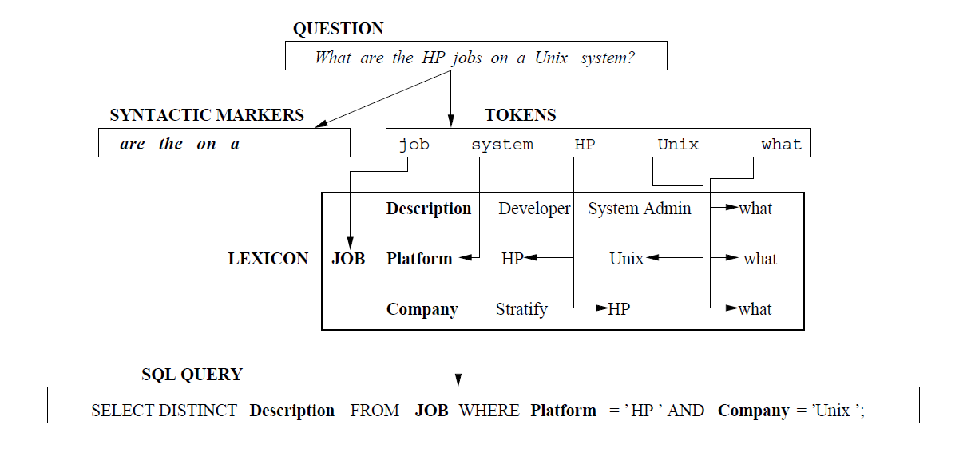
\includegraphics[scale=1.0]{graficos/popescu-example}
    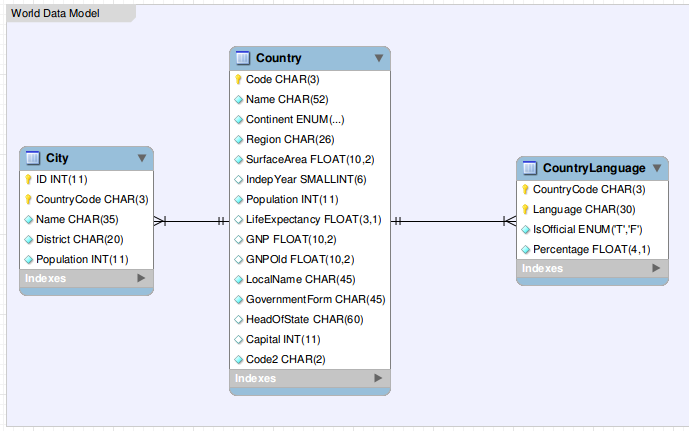
\includegraphics[width=12.823cm,height=8.004cm]{graficos/fuentes/world-db.png}
  \caption{Modelo entidad relación de la base de datos World original}
  \label{fig:world-db}
\end{figure}

La tabla Country tiene información básica acerca de varios países del mundo. La tabla City tiene información sobre las mayores ciudades del mundo y, finalmente, la tabla CountryLanguage tiene información sobre los idiomas hablados en cada país.

Hay una relación de uno a muchos entre Country y CountryLanguage: cada país puede tener más de un idioma y, además, hay una relación de uno a muchos entre Country y City: cada país puede tener más de una ciudad.

\medskip
Las definiciones de las relaciones originales son:
\begin{itemize}
\item Country(Code, Name, Continent, Region, SurfaceArea, IndepYear, Population, LifeExpectancy, GNP, GNPOld, LocalName, GovernmentForm, HeadOfState, Capital, Code2)
\item City(ID, ContryCode, Name, District, Population)
\item CountryLanguage(CountryCode, Language, IsOfficial, Percentage)
\end{itemize}

Para nuestro proyecto, renombramos algunos de los elementos:
\begin{itemize}
\item La relación CountryLanguage fue renombrada a Language
\item El atributo Language de la relación CountryLanguage fue renombrado a Name
\item El atributo IndepYear de la relación Country fue renombrado a IndependenceYear
\end{itemize}

Por otro lado, dado que, por una cuestión de tiempos y de complejidad del desarrollo, no soportamos más de un join posible entre tablas, eliminamos la referencia a la tabla City en el atributo Country.Capital. Lo que hicimos fue rellenar ese campo con el nombre de la ciudad en lugar de su  ID, perdiendo la posiblidad de navegar con preguntas del tipo ¿Cuál es la población de la capital del país X?.
Los JOINS que manejamos, en caso de ser necesarios por estarse refiriendo más de una tabla, son City.CountryCode $=$ Country.Code y Language.CountryCode$=$Country.Code.

En las tablas \ref{table:countrylanguage-data}, \ref{table:city-data}, \ref{tab:country-data} y \ref{tab:country-data-2} pueden verse algunas filas de ejemplo de cada una de las tablas.


 \begin{longtable}{|l|l|l|l|}
 \hline  \multicolumn{1}{|c|}{\textbf{CountryCode}} & \multicolumn{1}{|c|}{\textbf{Language}} & \multicolumn{1}{|c|}{\textbf{IsOfficial}} & \multicolumn{1}{|c|}{\textbf{Percentage}} \\ \hline  \endfirsthead
\caption{Algunas filas de la tabla CountryLanguage (cont)} \\ \hline \multicolumn{1}{|c|}{\textbf{CountryCode}} & \multicolumn{1}{|c|}{\textbf{Language}} & \multicolumn{1}{|c|}{\textbf{IsOfficial}} & \multicolumn{1}{|c|}{\textbf{Percentage}} \\ \hline \hline \endhead \endfoot
ABW & Dutch & T & 5.3 \\ \hline
ABW & English & F & 9.5 \\ \hline
ABW & Papiamento & F & 76.7 \\ \hline
ABW & Spanish & F & 7.4 \\ \hline
AFG & Balochi & F & 0.9 \\ \hline
AFG & Dari & T & 32.1 \\ \hline
AFG & Pashto & T & 52.4 \\ \hline
AFG & Turkmenian & F & 1.9 \\ \hline
AFG & Uzbek & F & 8.8 \\ \hline
AGO & Ambo & F & 2.4 \\ \hline
AGO & Chokwe & F & 4.2 \\ \hline
AGO & Kongo & F & 13.2 \\ \hline
AGO & Luchazi & F & 2.4 \\ \hline
\caption{Algunas filas de la tabla CountryLanguage}
\label{table:countrylanguage-data}
\end{longtable}



  \begin{longtable}{|l|l|l|l|l|}
 \hline \multicolumn{1}{|c|}{\textbf{ID}} & \multicolumn{1}{|c|}{\textbf{Name}} & \multicolumn{1}{|c|}{\textbf{CountryCode}} & \multicolumn{1}{|c|}{\textbf{District}} & \multicolumn{1}{|c|}{\textbf{Population}} \\ \hline \endfirsthead
\caption{Algunas filas de la tabla city} \\ \hline \multicolumn{1}{|c|}{\textbf{ID}} & \multicolumn{1}{|c|}{\textbf{Name}} & \multicolumn{1}{|c|}{\textbf{CountryCode}} & \multicolumn{1}{|c|}{\textbf{District}} & \multicolumn{1}{|c|}{\textbf{Population}} \\ \hline \hline \endhead \endfoot
129 & Oranjestad & ABW & – & 29034 \\ \hline
1 & Kabul & AFG & Kabol & 1780000 \\ \hline
56 & Luanda & AGO & Luanda & 2022000 \\ \hline
61 & South Hill & AIA & – & 961 \\ \hline
34 & Tirana & ALB & Tirana & 270000 \\ \hline
55 & Andorra la Vella & AND & Andorra la Vella & 21189 \\ \hline
33 & Willemstad & ANT & Curaçao & 2345 \\ \hline
64 & Dubai & ARE & Dubai & 669181 \\ \hline
69 & Buenos Aires & ARG & Distrito Federal & 2982146 \\ \hline
126 & Yerevan & ARM & Yerevan & 1248700 \\ \hline
53 & Tafuna & ASM & Tutuila & 5200 \\ \hline
63 & Saint John's & ATG & St John & 24000 \\ \hline
130 & Sydney & AUS & New South Wales & 3276207 \\ \hline
 \caption{Algunas filas de la relación City} \label{table:city-data}
 \end{longtable}

\bigskip


\begin{footnotesize}
 \begin{longtable}{|l|l|l|l|l|l|}
 \hline \multicolumn{1}{|c|}{\textbf{Code}} & \multicolumn{1}{|c|}{\textbf{Name}} & \multicolumn{1}{|c|}{\textbf{Continent}} & \multicolumn{1}{|c|}{\textbf{Region}} & \multicolumn{1}{|c|}{\textbf{SurfaceArea}} & \multicolumn{1}{|c|}{\textbf{IndepYear}} \\ \hline \hline  \endfirsthead
\caption{Algunas filas de la tabla Country} \\ \hline \multicolumn{1}{|c|}{\textbf{Code}} & \multicolumn{1}{|c|}{\textbf{Name}} & \multicolumn{1}{|c|}{\textbf{Continent}} & \multicolumn{1}{|c|}{\textbf{Region}} & \multicolumn{1}{|c|}{\textbf{SurfaceArea}} & \multicolumn{1}{|c|}{\textbf{IndepYear}} \\ \hline \hline \endhead \endfoot
ABW & Aruba & North America & Caribbean & 193.00 & \textit{NULL} \\ \hline
AFG & Afghanistan & Asia & Southern and Central Asia & 652090.00 & 1919 \\ \hline
AGO & Angola & Africa & Central Africa & 1246700.00 & 1975 \\ \hline
AIA & Anguilla & North America & Caribbean & 96.00 & \textit{NULL} \\ \hline
ALB & Albania & Europe & Southern Europe & 28748.00 & 1912 \\ \hline
AND & Andorra & Europe & Southern Europe & 468.00 & 1278 \\ \hline
ANT & Netherlands Antilles & North America & Caribbean & 800.00 & \textit{NULL} \\ \hline
ARE & United Arab Emirates & Asia & Middle East & 83600.00 & 1971 \\ \hline
ARG & Argentina & South America & South America & 2780400.00 & 1816 \\ \hline
ARM & Armenia & Asia & Middle East & 29800.00 & 1991 \\ \hline
ASM & American Samoa & Oceania & Polynesia & 199.00 & \textit{NULL} \\ \hline
ATA & Antarctica & Antarctica & Antarctica & 13120000.00 & \textit{NULL} \\ \hline
ATF & French Southern territories & Antarctica & Antarctica & 7780.00 & \textit{NULL} \\ \hline
 \caption{Algunas filas de la tabla Country} \label{tab:country-data}
 \end{longtable}
  \end{footnotesize}

\begin{footnotesize}
 \begin{longtable}{|l|l|p{2cm}|l|p {3cm}| p {3cm}|l|}
 \hline \multicolumn{1}{|c|}{\textbf{Code}} & \multicolumn{1}{|c|}{\textbf{Population}} & \multicolumn{1}{|p{2cm}|}{\textbf{Life Expectancy}} & \multicolumn{1}{|c|}{\textbf{GNP}} & \multicolumn{1}{|p {3cm}|}{\textbf{GovernmentForm}} & \multicolumn{1}{|p {3cm}|}{\textbf{HeadOfState}} & \multicolumn{1}{|c|}{\textbf{Capital}} \\ \hline \hline  \endfirsthead
\caption{Algunas filas de la tabla Country (continuación)} \\ \hline \multicolumn{1}{|c|}{\textbf{Code}} & \multicolumn{1}{|c|}{\textbf{Population}} & \multicolumn{1}{|c|}{\textbf{LifeExpectancy}} & \multicolumn{1}{|c|}{\textbf{GNP}} & \multicolumn{1}{|c|}{\textbf{GovernmentForm}} & \multicolumn{1}{|c|}{\textbf{HeadOfState}} & \multicolumn{1}{|c|}{\textbf{Capital}} \\ \hline \hline \endhead \endfoot
ABW & 103000 & 78.4 & 828.00 & Nonmetropolitan Territory of The Netherlands & Beatrix & 129 \\ \hline
AFG & 22720000 & 45.9 & 5976.00 & Islamic Emirate & Mohammad Omar & 1 \\ \hline
AGO & 12878000 & 38.3 & 6648.00 & Republic & José Eduardo dos Santos & 56 \\ \hline
AIA & 8000 & 76.1 & 63.20 & Dependent Territory of the UK & Elisabeth II & 62 \\ \hline
ALB & 3401200 & 71.6 & 3205.00 & Republic & Rexhep Mejdani & 34 \\ \hline
AND & 78000 & 83.5 & 1630.00 & Parliamentary Coprincipality &  & 55 \\ \hline
ANT & 217000 & 74.7 & 1941.00 & Nonmetropolitan Territory of The Netherlands & Beatrix & 33 \\ \hline
ARE & 2441000 & 74.1 & 37966.00 & Emirate Federation & Zayid bin Sultan al-Nahayan & 65 \\ \hline
ARG & 37032000 & 75.1 & 340238.00 & Federal Republic & Fernando de la Rúa & 69 \\ \hline
ARM & 3520000 & 66.4 & 1813.00 & Republic & Robert Kotšarjan & 126 \\ \hline
 \caption{Algunas filas de la tabla Country (continuación)} \label{tab:country-data-2}
 \end{longtable}
 \end{footnotesize}



Incorporando estos datos al modelo teórico, hasta aquí tenemos definidos: la base de datos, sus elementos ($E$) y el tipo de sus elementos.


\section{Implementación}
\label{sec:popescu-implementacion}


Estructuramos esta sección como sigue. Primero (\ref{subsec:popescu-codigo}), discutimos la implementación en sí misma, analizando los módulos más importantes del sistema, luego (\ref{subsec:popescu-ejemplos}) mostramos y comentamos algunos ejemplos de ejecuciones y, finalmente (\ref{subsec:popescu-cierre}), analizamos alcances, límites y trabajo futuro.

Este apartado es probablemente el más áspero y técnico de la tesis. Si la cantidad de conceptos presentada se vuelve demasiado difícil de reterner al lector, recomendamos saltear la sección de \allref{subsec:popescu-codigo} y comenzar por \allref{subsec:popescu-ejemplos}, o bien darle una primera lectura aproximativa a ref{subsec:popescu-codigo}, pasar a los ejempos un principio más por arriba y luego sí leer en detalle \ref{subsec:popescu-codigo}.

\subsection{Código}
\label{subsec:popescu-codigo}

\subsubsection*{Lexicón}
\label{subsubsec:lexicon}
El lexicón, recordemos, es el módulo encargado de generar un conjunto de tokens para cada  elemento de la base de datos. Una vez construido este conjunto, las responsabilidades del módulo son las siguientes:
\begin{itemize}
	\item Dado un lema, devolver el conjunto de tokens que lo contienen
	\item Dado un token, devolver el conjunto de elementos de la base de datos que le \textit{corresponden}.
\end{itemize}

El lexicón está implementado en la clase $uba.modules.Lexicon$. Debemos distinguir los momentos de construcción y de consulta del mismo. La construcción, cuyo punto de entrada es el módulo $uba.app.CreateLexicon$, ocurre por separado, y debe ejecutarse una vez antes de poder utilizar el sistema para responder preguntas. Esta genera 4 archivos con formato json, que son luego cargados en memoria al momento de realizar consultas.

En el centro la construcción del lexicón se encuentra Wordnet, una base de datos léxica en inglés, que consta de conjuntos de sinónimos, definiciones de los mismos y relaciones semánticas entre ellos. Utilizamos esta base de datos para obtener los sinónimos de los elementos de la base de datos.

El input del algoritmo es la lista de los elementos de la base de datos (relaciones, atributos y valores) como strings. El primer paso es eliminar el camel case y separar y lematizar las palabras (la tokenizamos en el sentido dado por Popescu a token). Por ejemplo, después de este paso, el elemento GovernmentForm se convierte en el token \{government, form\}. En este paso eliminamos también las stopwords (por ejemplo, HeadOfState se convierte en \{head, state\}).

Luego, los datos pasan por el TokenAugmenter, que simplemente agrega algunos sinónimos escritos a mano a algunos de estos elementos (ver tabla \ref{table:token-augmenter}). Por ejemplo, para el elemento ``region'' (atributo de la relación ``country''), agregamos el término ``location'', para el elemento ``surface area'' agregamos los términos ``total size'' y ``square kilometers''. Este paso es llevado a cabo por la clase $uba.db.TokenAugmenter$ y su intención es mejorar las chances de obtener sinónimos útiles a partir de wordnet, ampliando su input de trabajo. Al salir del TokenAugmenter tenemos, para cada elemento de la base de datos, un conjunto (que puede tener un solo string si el TokenAugmenter no tenía ningún sinónimo) de tokens (que son, a su vez, listas de lemas).

\begin{center}
\begin{table}[h]
\centering
\begin{tabular}{| l |  p{12cm} |}
\hline
Elemento original & Sinónimos \\ \hline
head of state & president, leader, emperor, king \\ \hline
region & location\\ \hline
surface area & size, total size, square kilometers, km2\\ \hline
independence year & independent, independency\\ \hline
\end{tabular}
\caption{Sinónimos introducidos por el Token Augmenter}
\label{table:token-augmenter}
\end{table}
\end{center}

El tercer paso es el central: en este se obtienen, para cada uno de estos tokens, tokens sinónimos. Para esto obtenemos una lista de sinónimos y palabras relacionadas para cada lema del token, luego los combinamos formando todos los sinónimos ordenados. Por ejemplo, si el token original consistía de los lemas (A, B) y para A obtuvimos los sinónimos \{A1, A2\} y para B los sinónimos \{B1 y B2\}, el resultado serán todas las combinaciones ordenadas posibles: \{(A, B), (A, B1), (A, B2), (A1, B), (A1, B1), (A1, B2), (A2, B), (A2, B1), (A2, B2)\}.

Finalmente, intentamos obtener sinónimos también de todas las palabras del token juntas (incluyendo las stopwords), ya que verificamos empíricamente que para algunas de ellas existía una entrada en wordnet (Por ejemplo ``head of state'' produce el sinónimo ``chief of state'' que se pierde sin este paso).

El conjunto de tokens sinónimos para cada elementos de la base de datos es luego invertido, es decir, en lugar de disponer de un mapeo de elementos de la base de datos a conjunto de tokens sinónimos, construimos un mapeo de tokens en elementos de la base de datos.

Vale mencionar que en este índice invertido agregamos también tokens para cada qword posible, mapeando a un solo elemento especial, de tipado similar a un valor (WhValue), mediante el cual los tokens de qwords acceden al espacio de elementos de la base de datos. Además, para estos WhValues definimos a mano la relación de compatibilidad con atributos de la base de datos tal como se define en los papers. Esta relación está definida en la clase $uba.db.WhGenerator$ tal como la presentamos en la tabla \ref{table:atributos-qwords}.

El proceso del Lexicón se hace offline y con él queda construido el espacio semántico disponible para comprender palabras.

\begin{center}
\begin{table}[h]
\centering
\begin{tabular}{| l |  p{12cm} |}
\hline
Qword & Atributos relacionados \\ \hline
What & \textbf{Name}, District, Population, Code, Continent, SurfaceArea, LifeExpectancy, GNP, LocalName, GovernmentForm,
                         Capital, IsOfficial, Percentage, Region \\ \hline
Which & Los mismos que para what\\ \hline
Where & \textbf{Region}, Continent, Capital, District\\ \hline
Who & \textbf{HeadOfState}\\ \hline
When & \textbf{IndependenceYear}\\ \hline
\end{tabular}
\caption{Atributos compatibles con cada Qword}
\label{table:atributos-qwords}
\end{table}
\end{center}

A partir de este mapeo son generadas algunas estructuras utilizadas para optimizar la performance del sistema, pero sin valor teórico (por ejemplo, la lista de todos los tokens, que es también el conjunto de índices del índice invertido). Estos datos son finalmente grabados en 4 archivos, que son luego cargados a memoria en el sistema principal.

Desde la perspectiva de la lectura, las operaciones son triviales. La interfaz de servicios ofrece los métodos getTokens() y getMatchingElements(). getTokens() es la encargada de devolver, para un lema, el conjunto de tokens que lo contienen, mientras que getMatchingElements() es la encargada de devolver, dado un token, el conjunto de elementos de la base de datos que le corresponden.

Discutamos ahora la implementación del tercer paso, en el que se obtienen sinónimos y palabras relacionadas para cada lema y luego se combinan.

En el caso ideal, lo que se busca es lograr un conjunto de sinónimos para una serie de palabras. Pero lo que entendemos por conjunto de sinónimos se ve opacado por un fenómeno lingüístico conocido como polisemia que es, en algún sentido, un fenómeno inverso a la sinonímia. Al utilizar wordnet siempre existe este problema. La polisemia refiere al hecho de que una palabra puede tener más de un sentido. Es el caso de la palabra banco, que puede ser tanto un asiento en una plaza como una institución financiera. La polisemia es un fenómeno que ocurre en el espacio de relaciones entre las palabras y los conceptos, al igual que la sinonímia, que refiere al hecho de que diferentes palabras pueden referir al mismo concepto (inodoro y retrete). En el core de wordnet existe el tipo de dato synset (conjunto de sinónimos, a veces traducido como anillo de sinónimos), en el que se agrupan, bajo un sentido o concepto, todas las palabras que lo refieren.

En general, los humanos podemos distinguir qué sentido de una palabra polisémica está en uso por contexto. Entre nuestras funciones cognitivas está el reconocer que si alguien dice ``voy a hacer un depósito al banco'', nosotros entendamos que banco, en este contexto, refiere a la institución financiera y no al asiento de plaza. Pero sin contexto es imposible saber de qué sentido se está hablando.

Este problema no es tematizado en los trabajos de Popescu y, sin embargo, ellos argumentan que el sistema Precise fue construido con wordnet (sin  mencionar ningún tipo de desambiguador contextual previo).
En realidad, existe un atenuante para este problema que es el contexto de uso y el rol que cumplen los conjuntos de sinónimos y es que el conjunto de todos los tokens sinónimos generados funciona como un filtro sobre consultas del usuario y nunca es activo o productivo.
Consideremos, por ejemplo, una base de datos sobre localización de sucursales de bancos y el elemento Banco (por ejemplo, el nombre de una relación).
Buscando en sinonimos.com obtenemos los siguientes sinónimos, separados en dos líneas: 1) entidad crediticia, 2) taburete, escabel, escaño, peana, sitial, asiento. Tomando todos los sinónimos tendríamos el siguiente conjunto de sinónimos: \{banco, entidad crediticia, taburete, escaño, peana, sitial, asiento\} donde hay, mezclados, dos sentidos. Ahora bien: ¿qué uso hacemos de este conjunto? El usuario de una aplicación sobre localización de bancos introduce una pregunta, el sistema la separa, lematiza y chequea si los lemas pertenecen a algún conjunto de sinónimos. En este contexto, ¿es un problema que tengamos el término ``asiento'' en nuestro conjunto de sinónimos? Sería un problema solo si el usuario pudiese introducirlo, ya que al conjunto de sinónimos solo se accede a partir de palabras introducidas por el usuario. Si bien este problema es posible, no es probable y, quizás, siguiendo este razonamiento, quienes propusieron el modelo no hicieron ningún énfasis en él.

Nuestro sistema no introduce ningún desambiguador de sentido: utilizamos todo los sinónimos disponibles de tipo sustantivo, introduciendo potenciales errores de interpretación en este punto, con la salvedad recién mencionada.


Finalmente, agregamos también derivaciones léxicas lematizadas. Una derivación léxica es una variación de la palabra original que da otro sentido (relacionado) a la palabra original. Por ejemplo: existir, existencia, existencial, existiendo, existente son una serie de variaciones de la misma raíz.  Esta opción es experimental y puede activarse o desactivarse desde el archivo de configuración ($uba.app.Config$)

En la tabla \ref{table:sinonimos} pueden verse algunos ejemplos de los resultados.

\begin{center}
\begin{table}[h]
\centering
\begin{tabular}{| l |  p{9.5cm} | p{4cm} |} \hline
Lema & Sinónimos & Derivaciones léxicas\\ \hline
city 	&	metropolis, (urban, center)	&	citify, metropolitan\\ \hline
country	&	state, nation, land, commonwealth, res publica, body politic, rural area, area	&	--\\ \hline
language	&	language, linguistic communication, speech, speech communication, spoken communication, spoken language, voice communication, oral communication, lyric, words, linguistic process, terminology, nomenclature & lyricist, lyric, speak, terminological \\ \hline
region	&	region, part, area, neighborhood, realm	&	--\\ \hline
location	&	location, placement, locating, position, positioning, emplacement, localization, localisation, fix	&	locate, position, posit, emplace, localize, localise\\ \hline
continent	&	--	&	continental\\ \hline
gnp	&	gross national product	&	--\\ \hline
government	&	government, authorities, regime, governing, governance, government activity, administration, politics, political science	&	govern, political scientist\\ \hline
form	&	form, word form, signifier, descriptor, kind, sort, variety, shape, pattern, configuration, contour, conformation, human body, physical body, material body, soma, build, figure, physique, anatomy, bod, chassis, frame, flesh, cast, variant, strain, var., phase, class, grade, course, mannequin, manikin, mannikin, manakin	&	signify, sort, form, shape, pattern, contour, anatomic, anatomist, anatomical, shapely, variant\\ \hline
\end{tabular}
\caption{Lemas, sinónimos y derivaciones léxicas}
\label{table:sinonimos}
\end{table}
\end{center}

\subsubsection*{Tokenizer}
\label{subsubsec:tokenizer}

El Tokenizer en el modelo de Popescu, recordemos, es el encargado de generar todas las tokenizaciones completas de la pregunta y, para cada token, consultar al Lexicon y retornar la lista de elementos de la base de datos que le corresponden.

\medskip

El Tokenizer sigue el siguiente procedimiento:
\begin{enumerate}
\item Separar la pregunta en palabras, eliminar puntuaciones y pasar a lower case.
\item Lematizar las palabras. Para esto usamos Freeling
\item Eliminar marcadores sintácticos.
\item Para cada lema, obtener todos los tokens que lo contienen del Lexicon (método getTokens).
\item Para cada token potencial (resultado del paso anterior) verificar que todos sus lemas estén presentes en el conjunto de lemas de la pregunta original.
\item Generar el conjunto de partes de todos los tokens hasta aquí obtenidos\footnote{El conjunto de partes de un conjunto dado es otro conjunto formado por todos los subconjuntos del mismo. Por ejemplo, el conjunto de partes de A = \{1, 2, 3\} es: \{ $\varnothing$, \{1\}, \{2\}, \{3\}, \{1, 2\}, \{2, 3\}, \{1, 3\}, \{1, 2, 3\} \}}. \\ \\
	Probando con cada elemento del conjunto de partes en lugar de utilizar solamente el conjunto original podemos obtener subconjuntos que cumplan también la condiciones requeridas para considerarse una tokenización completa (evaluados en 7).
\item Para cada uno de estos subconjuntos, verificar 1) que sus tokens cubran completamente los lemas significativos de la pregunta original y 2) que no haya lemas repetidos entre los tokens.
\end{enumerate}

El resultado será un conjunto de tokenizaciones completas. Como se ve, respetamos casi al pie de la letra la implementación sugerida por Popescu. La obtención de los elementos de la base de datos que corresponden a los elementos, por una cuestión implementativa, quedó en manos del Matcher y no del Tokenizer. La implementación, de todos modos, del servicio, está en el Lexicon. Con este conjunto de tokenizaciones completas como input, será responsabilidad del Matcher decidir cuáles de ellas son traducciones válidas.

\subsubsection*{Matcher}
\label{subsubsec:matcher}

El Matcher, por su parte, toma las tokenizaciones completas generadas por el Tokenizer, construye el grafo que expusimos en la sección \ref{subsec:closed-domain} y ejecuta el algoritmo de max flow. El problema de max-flow es un problema de grafos que consiste en “enviar” el máximo flujo posible a través de un grafo dirigido con dos nodos especiales (fuente o source y sumidero o sink) y aristas con cierta capacidad mayor o igual que cero. Este flujo debe ir desde el nodo fuente al nodo sumidero, respetando las capacidades de las aristas y respetando que, para cada nodo, el flujo saliente no puede ser mayor al flujo entrante.

Existen diferentes algoritmos para resolver este problema. En nuestra implementación, tomamos un código libre disponible en internet (aquí: \url{http://web.mit.edu/~ecprice/acm/acm08/MaxFlow.java}).

Las aristas implicadas en el flujo máximo posible asocian 1) los tokens de valor y de atributo y los correspondientes elementos (valores y atributos, respectivamente) de la base de datos y 2) pares de valores y atributos entre sí.

Después de esto, buscamos otras soluciones posibles de máximo flujo, dado que cualquier solución que tenga como valor para el máximo flujo la cantidad de tokens de valor en la pregunta es, potencialmente, una traducción válida. Para hacer esto retiramos, ordenadamente, las aristas del grafo que ocurren entre la columna 2 y 3 (tokens de valor y valores de la db).

Cabe notarse aquí, como ya mencionamos anteriormente, que no soportamos en nuestra implementación la desambiguación de tokens de relación. Esto significa que: asumimos que un token de relación tiene un solo elemento relación asociado y no será necesario decidir si refiere a una relación u a otra. En todos los ejemplos de bases de datos que consideramos, esta asunción era verdadera (es decir, no existía un token de relación que necesite ser desambiguado) y por ello no implementamos esta capacidad del sistema, que quedará como trabajo futuro. Así mismo, no soportamos tokens multi tipados, prefiriendo relaciones sobre atributos y valores y atributos sobre valores (el caso implementativo es simple: require un grafo extra por cada combinación de tipos distintos por token). Los casos en que esta ambigüedad ocurría eran específicos y la solución no reportaba ninguna mejora cualitativa, por lo que lo dejamos de lado, quedando como una mejora futura.

\medskip

Finalmente, verificamos cuales de las soluciones con máximo flujo cumplen las condiciones requeridas para ser una traducción válida según enunciamos en \ref{subsec:closed-domain}:

\begin{enumerate}
\item Todos  los tokens de la tokenización tienen un único elemento de la base de datos asociado y no hay elementos de la base de datos repetidos. (Mapping.meetsConditionOne())
\item Cada token de atributo se relaciona con un único token de valor respetando que: (Mapping.meetsConditionTwo())
\begin{enumerate}
\item el atributo relacionado con el token de atributo y el valor relacionado con el token de valor son compatibles (esta condición está garantizada por el max-flow mismo)
\item ambos tokens están sintácticamente asociados
\end{enumerate}
\item Cada token de relación está relacionado a un token de atributo o bien a un token de valor, cumpliendo las siguientes condiciones: (Mapping.meetsConditionThree())
\begin{enumerate}
\item	la relación de la base de datos que corresponde al token de relación y el elemento de la base de datos que corresponde al token de atributo o token de valor son compatibles
\item ambos tokens (token de relación - token de atributo o bien token de relación - token de valor) están sintácticamente asociados
\end{enumerate}
\item La pregunta tiene una qword (Mapping.hasOneWhValue())
\end{enumerate}

Notemos que la condición 3 implica que para cada token de relación exista algún token de atributo o de valor a) compatible y b) sintácticamente asociado. La condición a) no está verificada por el algoritmo de máximo flujo y es verificada en el método Mapping.valid()

Para verificar las condiciones de asociación sintáctica (2.b y 3.b) utilizamos la implementación oficial del árbol sintáctico de Charniak (\url{github.com/BLLIP/bllip-parser}), con un wrapper en java que es la clase $uba.nlp.CharniakParseTree$. Las reglas sintácticas utilizadas por Precise no están especificadas en los trabajos, por lo que creamos nuestras propias reglas tomando los ejemplos de asociaciones sintácticas dadas en los trabajos, evaluando los resultados de diferentes ejemplos y extrapolando reglas a partir de allí.


Veamos, en primer lugar, ejemplos del parse tree para tres preguntas:


\begin{center}
\Tree [.S1 [.SBARQ [.WHNP [.WP What ] ] [.SQ [.VP [.AUX are ] [.NP [.DT the ] [.NNP HP ] [.NNS jobs ] ] [.PP [.IN on ] [.NP [.DT a ] [.NNP Unix ] [.NN system ] ] ] ] ] [.. ? ] ] ] \\
``What are the HP jobs on a Unix system?''
\end{center}

\begin{center}

\Tree [.S1 [.SBARQ [.WHNP [.WP What ] ] [.SQ [.VP [.AUX are ] [.NP [.NP [.DT the ] [.NNS capitals ] ] [.PP [.IN of ] [.NP [.DT the ] [.NNP US ] [.NNS states ] ] ] ] ] ] [.. ? ] ] ] \\
``What are the capitals of the US states?''
\end{center}


\begin{center}
\Tree [.S1 [.SBARQ [.WHNP [.WP What ] ] [.SQ [.VP [.AUX are ] [.NP [.NP [.DT the ] [.NNS names ] ] [.PP [.IN of ] [.NP [.NP [.NNS cities ] ] [.PP [.IN of ] [.NP [.NNP Argentina ] ] ] ] ] ] ] ] [.. ? ] ] ]\\
``What are the names of cities of Argentina?''
\end{center}

En las figuras \ref{fig:word-tags} y \ref{fig:syntax-tags} pueden verse los diferentes tags para hojas y para nodos intermedios (respectivamente).


\begin{figure}[H]
  \centering
    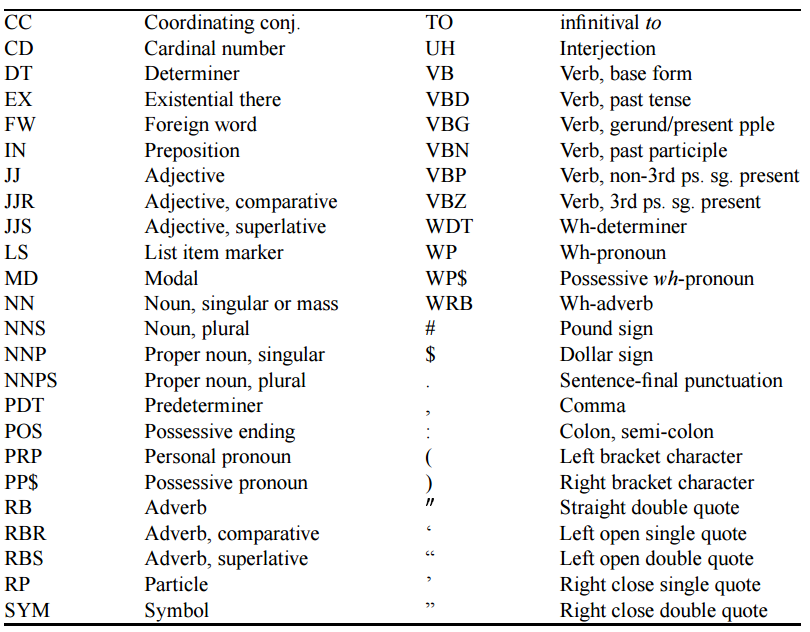
\includegraphics[width=12.823cm,height=8.004cm]{graficos/fuentes/WordTags.png}
  \caption{POS tags de Penn Treebank}
  \label{fig:word-tags}
\end{figure}


\begin{figure}[H]
  \centering
    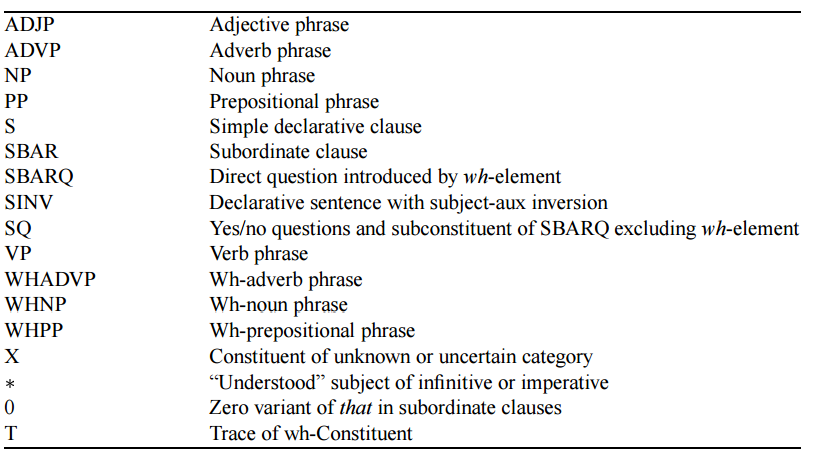
\includegraphics[width=12.823cm,height=8.004cm]{graficos/fuentes/SyntaxTags.png}
  \caption{Conjunto de tags para nodos intermedios del árbol sintáctico}
  \label{fig:syntax-tags}
\end{figure}


Las reglas que construimos son las siguientes (notar que los nombres pueden denotar una direccionalidad, pero las relaciones son simétricas).
Utilizamos NNx para denotar cualquier hoja sustantivo, adjetivo o adverbio (JJ, JJR, JJS, NN, NNS, NNP, NNPS, RB, RBR, RBS, CD), NN para denotar estrictamente sustantivos (NN, NNS, NNP, NNPS), Nx para denotar cualquier sintagma relacionado a estos tipos de hojas (nodos intermedios): (ADJP, ADVP, NP, S) y Wx para denotar alguna de estas hojas: WDT, WP, WP\$ y WRB.

\begin{enumerate}
\item Hermanos:
  \begin{itemize}
    \item  NNx $\Leftrightarrow$ NNx $\Leftrightarrow$ Wx si comparten el mismo el mismo padre
  \end{itemize}
\item Qwords a sustantivo:
  \begin{itemize}
    \item Una Wx dentro de un WHNP $\Rightarrow$ un NN dentro de uno o más Nx dentro de un VP dentro de un SQ con el mismo SBARQ como padre que la WHNP mencionada.
  \end{itemize}
\item Sintagma nominal a sintagma preposicional:
  \begin{itemize}
    \item NN dentro de un Nx (1) $\Rightarrow$ NNx dentro de uno o más Nx dentro de un PP con el mismo padre que el Nx marcado con el (1)
  \end{itemize}
\item Sintagma nominal a sintagma verbal
    \begin{itemize}
      \item NN dentro de un Nx (1) $\Rightarrow$ NNx dentro de uno o más Nx dentro de un VP del mismo padre que el Nx marcado con el (1)
    \end{itemize}
\item Sintagma preposicional a sintagma preposicional:
  \begin{itemize}
    \item NNx dentro de un PP (1) $\Rightarrow$ NNx dentro de uno o más Nx dentro de un PP con el mismo padre que el PP marcado con el (1)
  \end{itemize}
  \item Términos a tokens:
  \begin{itemize}
    \item Dos tokens están asociados si cualquier término de uno está asociado a cualquier término de otro.
  \end{itemize}
\end{enumerate}

En los ejemplos presentados, los pares de términos asociados según estas reglas son los siguientes. Para el primero, (hp, jobs), (unix, system)  (regla 1), (what, hp), (what, jobs) (regla 2) y, finalmente, (hp, unix), (hp, system), (job, unix), (jobs, system) (regla 3). Para el segundo, (us, states) (regla 1), (what, capitals) (regla 2) y (capitals, us) y (capitals, states) (regla 3). Para el tercero, (what, names) (regla 2), (names, cities) y (cities, argentina) (regla 3).
\newline

La definición de las reglas se hizo a prueba y error y es posible que sea simple, para alguien con mayores conocimientos lingüísticos, mejorarlas. Probablemente tenga sentido diferenciar entre sustantivos principal y modificador (Unix y system, por ejemplo) y modificar las reglas 3 y 4 para conectar solo los principales, entre otras mejoras. El sistema ofrece también la opción de no evaluar las asociaciones sintácticas en absoluto, en cuyo caso se mejora la performance pero aparecen nuevas traducciones válidas que podrían haber sido filtradas por estas condiciones, que el usuario deberá desambiguar manualmente).
Además, estas reglas seguramente sean insuficientes y estén dejando afuera varias preguntas que deberían poder procesarse.

Finalmente, todos los resultados de max-flow que cumplen con las condiciones de 1 a  4 son traducciones válidas, que pasan al MappingFilter, que realiza ciertos filtrados que describiremos, de nuevo, en un título aparte.

El resultado de este módulo es una lista de Mappings (una estructura que contiene 1) una tokenización completa de la pregunta original y 2) un mapeo válido entre cada token de la misma en un elemento de la base de datos). Cada mapeo es una traducción válida de la pregunta. Si existe solo uno, entonces este mapeo se traducirá en una query que generará el resultado. Si no, corresponde al MappingFilter realizar filtrados inteligentes de las múltiples soluciones y, en caso de que continuen existiendo múltiples soluciones, entonces se consultará al usuario qué quiso preguntar. Por otro lado, si no fue posible generar ninguna traducción válida, se retornará al usuario sin respuesta, pidiéndole que vuelva a escribir su pregunta de otro modo.

\subsubsection*{MappingFilter}
\label{subsubsec:mapping-filter}

La clase $uba.app.MappingFilter$ es responsable, en primer lugar, de quitar las traducciones válidas repetidas y, en segundo lugar, de aplicar una serie de reglas también de filtrado. Para eliminar las traducciones repetidas, las transformamos en queries y simplemente comparamos por igualdad, ya que el generador de queries ordena las cláusulas generando, para inputs iguales pero diferentemente ordenados, la misma query.
Además de este filtro, aplicamos tres reglas más, de creación propia. En primer lugar, eliminamos ``semi duplicados'', que consisten en atributos similares en la base de datos, en concreto, para esta base de datos, consideramos semi-duplicada a una query que consulta por Country.Name y por Country.LocalName solamente. La segunda y la tercera regla están basadas en la siguiente idea: en el caso en que exista más de una traducción válida en la cual la qword esté asociada con un atributo \textit{implícito}, por como está el sistema definido, también estará asociado con todos los atributos que pueda estarlo (ver tabla \allref{table:atributos-qwords} para las compatibilidades definidas). Esto implica que, por ejemplo, para cualquier pregunta cuya qword sea 'what' y no tenga su atributo asociado explícito, habrá 16 diferentes traducciones válidas. En los trabajos sobre los que basamos nuestro proyecto este problema no está mencionado y en los ejemplos presentados no es visible. Lo que hicimos en este caso es aplicar dos conceptos de preferencia. La segunda regla prefiere, entre los atributos implícitos posibles, aquellos cuya relación está mencionada en la pregunta (si hubiera alguna). La tercer regla señala un orden de preferencia entre los atributos mismos, una vez especificada la relación. El atributo implicito preferido está marcado en negrita en la tabla \ref{table:atributos-qwords}. Si tras aplicar estar reglas siguen existiendo más de una traducción válida, entonces damos al usuario el control, pidiendo por una desambiguación.


\subsubsection*{QueryGenerator}
\label{subsubsec:query-generator}

El procedimiento para generar una query a partir de una traducción válida es exactamente el mismo que se desarrollo en \ref{subsec:closed-domain} y está implementado en el método Mapping.query().


\subsubsection*{MainProcessor}
\label{subsubsec:main-processor}

Finalmente, el punto de entrada de todo el sistema es $uba.app.MainProcessor$, que puede utilizarse especificando el parámetro -q QUESTION en cuyo caso responderá a esa pregunta y retornará el control o bien sin parámetros, en cuyo caso ingresa en un loop de preguntas-respuestas. El resultado para cada pregunta es cero, una o más queries de SQL.
Agregamos la opción de desambiguación para que el usuario elija entre dos o más queries si no se pudo generar una y también una presentación de las respuestas una vez determinada la query final, pero es más bien experimental y poco sólido.

\subsection{Ejemplos}
\label{subsec:popescu-ejemplos}

\subsubsection*{Ejemplo 1: ``Who is the head of state of Zimbabwe?''}

Consideremos nuestro primer ejemplo, una corrida trivial: ``Who is the head of state of Zimbabwe?''.

El primer paso es el tokenizer que, según expusimos, consta de los siguientes 7 pasos:

\begin{enumerate}
  \item Separar la pregunta en palabras, eliminar puntuaciones y pasar a lower case:
  \begin{itemize}
    \item \{who, is, the, head, of, state, of, zimbabwe\}
  \end{itemize}
  \item Lematizar las palabras:
  \begin{itemize}
    \item Todas las palabras ya están en su forma lematizada
  \end{itemize}
  \item Eliminar marcadores sintácticos:
  \begin{itemize}
    \item \{who, head, state, zimbabwe\}
  \end{itemize}
  \item Obtener tokens para cada lema ($Lexicon.getTokens()$)
  \begin{itemize}
    \item $getTokens(who)\ \rightarrow \{$'who'$\}$
    \item $getTokens(head)\ \rightarrow \{$ 'head country', 'head teacher body politic', 'head body politic', 'head teacher land', 'read / write head dos', 'heading provincial', 'heading state', 'heading commonwealth', 'head teacher dos', 'head teacher country', 'read / write head body politic', 'head word land', 'head state of matter', 'read / write head provincial', 'read / write head state department', 'read / write head department of state', 'head province', 'heading body politic', 'heading res publica', 'read / write head nation', (51 más)...$\}$

    \item $getTokens(state)\ \rightarrow  \{$'heart eastern united states', 'centre eastern united states', 'central eastern united states', 'centrical eastern united states', 'midsection eastern united states', 'midriff eastern united states', 'centric eastern united states', 'center eastern united states', 'middle eastern united states', 'eye eastern united states', 'camellia state yaman', 'frederick north western united states', 'compass north western united states', 'north western united states', 'second earl of guilford western united states', 'magnetic north western united states', 'northward western united states', 'due north western united states', 'union western united states', (702 más)...$\}$
    \item $getTokens(zimbabwe)\ \rightarrow \{$'zimbabwe', 'republic of zimbabwe', 'capital of zimbabwe'$\}$
  \end{itemize}
  \item Para cada token potencial (resultado del paso anterior) verificar que todos sus lemas estén presentes en el conjunto de lemas de la pregunta original.
  \begin{itemize}
    \item $getTokens(who)\ \rightarrow \{$'who'$\}$
    \item $getTokens(head)\ \rightarrow \{$'head state', 'heading state', 'head of state' $\}$
    \item $getTokens(state)\ \rightarrow  \{$  'state', 'head state', 'heading state', 'head of state'$\}$
    \item $getTokens(zimbabwe)\ \rightarrow \{$'zimbabwe'$\}$
  \end{itemize}
  \item Generar el conjunto de partes de todos los tokens hasta aquí obtenidos.
  \newline
  \{ $\emptyset$, \{'head of state', 'zimbabwe'\}, \{'zimbabwe', 'state'\}, \{'zimbabwe', 'heading state', 'state', 'head state', 'who'\}, \{'head of state', 'zimbabwe', 'who'\}, \{'head of state', 'zimbabwe', 'heading state', 'head state', 'who'\}, \{'head of state', 'zimbabwe', 'heading state', 'who'\}, \{'head of state', 'zimbabwe', 'heading state', 'state'\}, \{'head of state', 'zimbabwe', 'heading state', 'state', 'who'\}, \{'who'\}, \{'head of state', 'heading state', 'head state'\}, \{'head of state'\}, \{'state', 'who'\}, \{'head of state', 'zimbabwe', 'heading state', 'head state'\}, \{'heading state', 'state', 'who'\}, \{'heading state', 'state'\}, \{'heading state', 'who'\}, \{'head of state', 'who'\}, \{'head of state', 'zimbabwe', 'state', 'who'\}, \{'head of state', 'state', 'head state'\}, \{'zimbabwe', 'heading state', 'state', 'who'\}, \{'zimbabwe', 'head state', 'who'\}, \{'zimbabwe', 'heading state', 'who'\}, \{'head of state', 'heading state', 'who'\}, \{'state', 'head state', 'who'\}, \{'head state'\}, \{'heading state', 'state', 'head state'\}, \{'head of state', 'state', 'who'\}, \{'zimbabwe'\}, \{'state', 'head state'\}, \{'state'\}, \{'head of state', 'heading state', 'state'\}, \{'zimbabwe', 'state', 'who'\}, \{'zimbabwe', 'state', 'head state'\}, \{'head of state', 'zimbabwe', 'heading state', 'state', 'head state'\}, \{'head of state', 'zimbabwe', 'heading state', 'state', 'head state', 'who'\}, \{'head of state', 'zimbabwe', 'state', 'head state', 'who'\}, \{'heading state', 'head state', 'who'\}, \{'heading state'\}, \{'head of state', 'zimbabwe', 'state'\}, \{'head of state', 'zimbabwe', 'head state', 'who'\}, \{'head of state', 'heading state', 'state', 'who'\}, \{'head of state', 'zimbabwe', 'state', 'head state'\}, \{'head of state', 'zimbabwe', 'heading state'\}, \{'head of state', 'zimbabwe', 'head state'\}, \{'head of state', 'heading state', 'state', 'head state'\}, \{'head state', 'who'\}, \{'head of state', 'state'\}, \{'head of state', 'heading state', 'head state', 'who'\}, \{'head of state', 'heading state', 'state', 'head state', 'who'\}, \{'zimbabwe', 'heading state'\}, \{'head of state', 'head state'\}, \{'heading state', 'state', 'head state', 'who'\}, \{'zimbabwe', 'state', 'head state', 'who'\}, \{'heading state', 'head state'\}, \{'head of state', 'head state', 'who'\}, \{'head of state', 'heading state'\}, \{'zimbabwe', 'heading state', 'state'\}, \{'zimbabwe', 'heading state', 'head state', 'who'\}, \{'zimbabwe', 'who'\}, \{'zimbabwe', 'head state'\}, \{'zimbabwe', 'heading state', 'head state'\}, \{'zimbabwe', 'heading state', 'state', 'head state'\}, \{'head of state', 'state', 'head state', 'who'\} \}
  \item Para cada uno de estos subconjuntos, verificar 1) que los lemas de sus tokens cubran completamente
los lemas significativos de la pregunta original y 2) que no haya lemas repetidos
entre los tokens.
  \begin{itemize}
    \item Los lemas significativos son los obtenidos en el bullet 4: \{who, head, state, zimbabwe\}
    \item Las tokenizaciones que los cubren sin repetir lemas son: \{'who', 'head state', 'zimbabwe'\},
    \{'who', 'heading state', 'zimbabwe'\} y  \{'who', 'head of state', 'zimbabwe'\}, con lo que queda eliminado el token 'state' y las repeticiones de los tokens que refieren tanto a 'head' como a 'state', quedando solo las diferentes formulaciones sinónimas del mismo elemento de la base de datos.
  \end{itemize}
\end{enumerate}

Es decir, el Tokenizer encontró tres conjuntos de tokens completos para la pregunta, Tokenizer.generateCompleteTokenizations(``Who is the head of state of Zimbabwe?'') $\rightarrow$ [\{ `who', `head state', `zimbabwe'\}, \{`who', `heading state', `zimbabwe'\}, \{`who', `head of state', `zimbabwe'\}].

El siguiente paso es el Matcher, que construye el grafo de atributos y valores para cada uno de las tokenizaciones completas y decide si existe un conjunto de elementos de la base de datos que permita establecer la traducción. Presentamos aquí solamente el grafo para la primer tokenización completa, que puede verse en la figura \ref{grafo-1}. Las otras tokenizaciones tienen un grafo análogo y generaran el mismo resultado, que será filtrado luego por el EquivalenceChecker. Notar que no es esta repetición de tokenizaciones lo que filtra el Matcher, sino la ambigüedad introducida por un token que puede referir a dos o más elementos de la base de datos (este problema no ocurre en este primer ejemplo).
 Para construirlo, primero, se consulta al Lexicón por el tipo y los elementos asociados de cada token mediante el servicio $getMatchingElements$ como se puede ver en la tabla \ref{table:get-matching-elements-1}.
\begin{center}
\begin{table}[h]
\centering
\begin{tabular}{| p{3cm} | l | l | p{6cm} |}
\hline
Token & Tipos & Elementos & Detalle \\ \hline
zimbabwe & Value & Zimbabwe & Valor del Atributo Name de la tabla Country\\ \hline
head state, head of state, heading state & Attribute & HeadOfState & Atributo de la tabla Country\\ \hline
who & WhValue/Value & Who & Q-valor compatible con: Atributo HeadOfState de la tabla Country\\ \hline
\end{tabular}
\caption{Resultados de $getMatchingElements$ para ``Who is the head of state of Zimbabwe?''}
\label{table:get-matching-elements-1}
\end{table}
\end{center}

En este primer ejemplo el grafo no desambigua ninguna relación token-elemento ya que no hay ningún token con más de un elemento asociado, por lo que el grafo de max-flow no tiene ningun atractivo especial y es construido siguendo el procedimiento reseñado en \ref{subsec:closed-domain} Al ejecutar el algoritmo de max-flow sobre el grafo, se obtiene que el flujo máximo es 2 y los pares generados son (Who, Country.HeadOfState), (Country.Name, Zimbabwe), sin generar ningún otro flujo alternativo como se ve en la figura \ref{grafo-1}.

\begin{figure}
\hspace*{-1.2cm}
\centering
\begin{tikzpicture}
\small
\matrix [column sep=3mm, row sep=5mm] {
   & \node (title1) [] {Tokens Valor};
   & \node (title) [] {Valores DB};
   & \node (title) [] {Atributos DB};
   & \node (title) [] {Atributos DB-2};
   & \node (title) [] {Tokens Atributo};& &

  \\
     &  \node (token_zimbabwe) [draw, shape=rectangle] {zimbabwe}; & \node (value_zimbabwe) [draw, shape=rectangle] {Name=Zimbabwe}; & \node (attr_name_1) [draw, shape=rectangle] {Name}; &  \node (attr_name_2) [draw, shape=rectangle] {Name};& & \node (i) [draw, shape=circle] {I}; &

  \\
  \node (source) [draw, shape=circle] {S}; & & & & & & & &\node (sink) [draw, shape=circle] {T};
  \\
   &  \node (token_who) [draw, shape=rectangle] {who}; & \node (value_who) [draw, shape=rectangle] {HeadOfState=Who}; & \node (attr_head_1) [draw, shape=rectangle] {HeadOfState}; &  \node (attr_head_2) [draw, shape=rectangle] {HeadOfState};&
   \node (token_head) [draw, shape=rectangle] {head state}; &
   \node (e) [draw, shape=circle] {E}; &

   \\
};
\draw[->, thick] (source) -- (token_zimbabwe);
\draw[->, thick] (token_zimbabwe) -- (value_zimbabwe);
\draw[->, thick] (value_zimbabwe) -- (attr_name_1);
\draw[->, thick] (attr_name_1) -- (attr_name_2);
\draw[->, thick] (attr_name_2) -- (i);
\draw[->, thick] (source) -- (token_who);
\draw[->, thick] (token_who) -- (value_who);
\draw[->, thick] (value_who) -- (attr_head_1);
\draw[->, thick] (attr_head_1) -- (attr_head_2);
\draw[->, thick] (attr_head_2) -- (token_head);
\draw[->, thick] (token_head) -- (e);

\draw[->, thick] (i) -- (sink) node [near end, fill=white, above] {f=1};
\draw[->, thick] (e) -- (sink) node [near end, fill=white, below] {f=1};
\end{tikzpicture}
\caption{Grafo de atributo-valor para la primer tokenización completa de ``Who is the head of state of Zimbabwe?''}
\label{grafo-1}
\end{figure}

El próximo paso es evaluar que los términos del par de tokens (`who', `head state') estén sintácticamente asociados en el
parse tree generado por el algoritmo de Charniak según nuestras reglas. El arbol sintáctico para la pregunta es el siguiente:

\begin{center}
\Tree [.S1 [.SBARQ [.WHNP [.WP \textbf{Who} ] ] [.SQ [.VP [.AUX is ] [.NP [.NP [.DT the ] [.NN \textbf{head} ] ] [.PP [.IN of ] [.NP [.NN state ] ] ] [.PP [.IN of ] [.NP [.NNP Zimbabwe ] ] ] ] ] ] [.. ? ] ] ] \\
``Who is the head of state of Zimbabwe?''
\end{center}

La regla 2 (q-word a sustantivo) vincula los términos 'who' con 'head', mientras que la 6 (términos a tokens), asocia los tokens 'who' con 'head state', cumpliendo las condiciones sintácticas requeridas por la definición de traducción válida. Por su parte, el atributo Name es implícito, lo que significa que no posee ningún token asociado y, por lo tanto, no debe cumplir la regla de traducciones válidas. Además, como no hay ninguna relación mencionada explícitamente, los tokens cubren todos los términos significativos de la pregunta y no hay ningún término repetido entre los tokens, esto significa que tenemos una (única) traducción válida para esta tokenización completa, constando de los siguiente elementos de la base de datos apareados: (Atributo Country.Name, Valor Country.Name$=$Zimbabwe), (Atributo Country.HeadOfState, Q-Valor Who).

Las otras dos tokenizaciones generan la misma traducción y sus repeticiones son eliminadas por el $EquivalenceChecker$.

Finalmente, esta única traducción pasa al $QueryGenerator$ que, aplicando las reglas descriptas en \ref{subsec:closed-domain}, genera la siguiente consulta SQL:

\medskip 
\textbf{SELECT} Country.HeadOfState \textbf{FROM} Country \textbf{WHERE} Country.Name$=$`Zimbabwe'
\medskip


Cuyo resultado es ``Robert G. Mugabe''.



\subsubsection*{Ejemplo 2: ``What caribbean countries are also considered north american?''}

Consideremos nuestro segundo ejemplo: ``What caribbean countries are also considered north american?''.

El primer paso es el tokenizer que, según expusimos, consta de los siguientes 7 pasos:

\begin{enumerate}
  \item Separar la pregunta en palabras, eliminar puntuaciones y pasar a lower case:
  \begin{itemize}
    \item \{what, caribbean, countries, are, also, considered, north, american\}
  \end{itemize}
  \item Lematizar las palabras:
  \begin{itemize}
    \item \{what, caribbean, country, is, also, consider, north, american\}
  \end{itemize}
  \item Eliminar marcadores sintácticos:
  \begin{itemize}
    \item \{what, caribbean, country, north, american\}
  \end{itemize}
  \item Obtener tokens para cada lema ($Lexicon.getTokens()$)
  \begin{itemize}
    \item $getTokens(what)\ \rightarrow \{$'what'$\}$
    \item $getTokens(caribbean)\ \rightarrow \{$'caribbean sea', 'caribbean', 'micronesia caribbean sea', 'federated states of micronesia caribbean', 'tt caribbean sea', 'micronesia / caribbean', 'tt caribbean', 'micronesia caribbean', 'federated states of micronesia caribbean sea'$\}$
    \item $getTokens(country)\ \rightarrow  \{$'country codification', 'country computer code', 'country codify', 'country code', 'baltic country', 'baltic language country', 'baltic sea country', 'north germanic language country', 'norse country', 'nordic country', 'scandinavian country', 'scandinavian language country', 'north germanic country', 'independent christian church country', 'free lance christian church country', 'self - employed person church building country', 'freelance church country', 'independent church service country', 'freelancer churchly country', 'free - lance churchly country', (149 más)...$\}$
    \item $getTokens(north)\ \rightarrow \{$'jabir aluminum ahmad aluminum jabir heart of dixie north borneo', 'jabir alabama ahmad camellia state jabir aluminum north borneo', 'jabir aluminize ahmad aluminise jabir aluminous north borneo', 'jabir aluminium ahmad camellia state jabir aluminize north borneo', 'jabir aluminize ahmad camellia state jabir aluminise north borneo', 'jabir al ahmad al jabir aluminium north borneo', 'jabir aluminous ahmad al jabir aluminise north borneo', 'jabir heart of dixie ahmad aluminous jabir camellia state north borneo', 'jabir aluminous ahmad camellia state jabir aluminous north borneo', 'jabir aluminium ahmad al jabir aluminize north borneo', 'jabir al ahmad aluminize jabir alabama north borneo', 'jabir aluminous ahmad al jabir heart of dixie north borneo', 'jabir aluminum ahmad aluminous jabir aluminum north borneo', 'jabir aluminum ahmad alabama jabir al north borneo', 'jabir heart of dixie ahmad aluminise jabir aluminous north borneo', 'jabir atomic number 13 ahmad aluminum jabir atomic number 13 north borneo', 'jabir aluminise ahmad alabama jabir aluminum north borneo', 'jabir aluminum ahmad aluminize jabir aluminize north borneo', 'jabir aluminium ahmad al jabir aluminous north borneo', 'jabir aluminous ahmad aluminium jabir camellia state north borneo', (2237 más)...$\}$
    \item $getTokens(american)\ \rightarrow \{$ 'american virgin islands', 'southward american', 'south american', 'due south american', 's american', 'dixieland american', 'dixie american', 'confederate states of america american', 'confederacy american', 'confederate states american', 'northward american', 'due north american', 'frederick north american', 'n american', 'second earl of guilford american', 'union american', 'north american', 'compass north american', 'magnetic north american', 'american - indian language spoken language', (169 más)...$\}$
  \end{itemize}
  \item Para cada token potencial (resultado del paso anterior) verificar que todos sus lemas estén presentes en el conjunto de lemas de la pregunta original.
  \begin{itemize}
    \item $getTokens(what)\ \rightarrow \{$'what'$\}$
    \item $getTokens(caribbean)\ \rightarrow \{$'caribbean'$\}$
    \item $getTokens(country)\ \rightarrow  \{$'country'$\}$
    \item $getTokens(north)\ \rightarrow \{$'north american'$\}$
    \item $getTokens(american)\ \rightarrow \{$'north american', 'american'$\}$
  \end{itemize}
  \item Generar el conjunto de partes de todos los tokens hasta aquí obtenidos.
  \newline
   \{ $\emptyset$, \{'north american'\}, \{'what', 'american', 'country'\}, \{'north american', 'what', 'american', 'country'\}, \{'american', 'caribbean'\}, \{'north american', 'what', 'american'\}, \{'what', 'country'\}, \{'north american', 'what', 'american', 'caribbean', 'country'\}, \{'caribbean'\}, \{'north american', 'what', 'caribbean'\}, \{'north american', 'american', 'country'\}, \{'north american', 'what'\}, \{'american'\}, \{'north american', 'american', 'caribbean', 'country'\}, \{'north american', 'what', 'caribbean', 'country'\}, \{'american', 'country'\}, \{'what', 'american', 'caribbean', 'country'\}, \{'north american', 'country'\}, \{'what', 'american'\}, \{'what', 'caribbean', 'country'\}, \{'american', 'caribbean', 'country'\}, \{'north american', 'caribbean'\}, \{'country'\}, \{'north american', 'what', 'american', 'caribbean'\}, \{'north american', 'caribbean', 'country'\}, \{'north american', 'what', 'country'\}, \{'what', 'caribbean'\}, \{'north american', 'american', 'caribbean'\}, \{'what'\}, \{'north american', 'american'\}, \{'what', 'american', 'caribbean'\}, \{'caribbean', 'country'\}\}
  \item Para cada uno de estos subconjuntos, verificar 1) que los lemas de sus tokens cubran completamente
los lemas significativos de la pregunta original y 2) que no haya lemas repetidos
entre los tokens.
  \begin{itemize}
    \item Los lemas significativos son los obtenidos en el bullet 4: \{what, caribbean, country, north, american\}
    \item Solo una tokenización los cubren sin repetir lemas: \{'north american', 'what', 'caribbean', 'country'\}, con lo que queda eliminado el token 'american'.
  \end{itemize}
\end{enumerate}

Es decir, el Tokenizer encontró un conjunto de tokens completo para la pregunta, Tokenizer.generateCompleteTokenizations(``What caribbean countries are also considered north american?'') $\rightarrow$ [ \{what, caribbean, country, north american\}].

El siguiente paso es el grafo del Matcher, que en este caso sí desambigua un token de valor. Como puede verse en \ref{table:get-matching-elements-2}, al token 'caribbean' le corresponden dos posibles valores: valor del atributo Region de la tabla Country y también valor del atributo Continent de la tabla Country.

En este ejemplo el grafo decide entre dos interpretaciones posibles  (Ver grafo \ref{grafo-2}) para el token 'caribbean', que puede ser un valor tanto del atributo Region como del atributo Continent. Teniendo presente el token 'north american', que solo puede tomar el atributo Continent, para maximizar el flujo el algoritmo asigna 'caribean' a Region, obteniendo un flujo de 3, que es el máximo, eliminando así la posibilidad de relacionar este token de valor con el atributo Continent.

\begin{center}
\begin{table}[h]
\centering
\begin{tabular}{| p{2cm} | p{2cm} | p{2cm} | p{6cm} |}
\hline
Token & Tipos & Elementos & Detalle \\ \hline
caribbean & Value & North America & Valor de los Atributo Region y Continent de la tabla Country\\ \hline
north american & Value & Caribbean & Valor del Atributo Region de la tabla Country\\ \hline
country & Relation & Country & Relación Country\\ \hline
what & WhValue / Value & What & Q-valor compatible con: Atributos GovernmentForm, Population, GNP, Name, Capital, LocalName, Continent, Region, Code, LifeExpectancy y SurfaceArea de la tabla Country, District, Population y Name de la tabla City e ISOfficial y Percentage de la tabla Language\\ \hline
\end{tabular}
\caption{Resultados de $getMatchingElements$ para ``What caribbean countries are also considered north american?''}
\label{table:get-matching-elements-2}
\end{table}
\end{center}

\begin{figure}
\hspace*{-1.5cm}
\centering
\begin{tikzpicture}
\footnotesize
\matrix [column sep=3mm, row sep=5mm] {
   & \node (title1) [] {Tokens Valor};
   & \node (title) [] {Valores DB};
   & \node (title) [] {Atributos DB};
   & \node (title) [] {Atributos DB-2};
   & \node (title) [] {Tokens Atributo};& & \\

   &  \node (token_what) [draw, shape=rectangle] {what}; & \node (value_what) [draw, shape=rectangle] {Country.Name[i]*=What}; & \node (attr_name_1) [draw, shape=rectangle] {Name[i]}; &  \node (attr_name_2) [draw, shape=rectangle] {Name[i]}; & & \node (e) [draw, shape=circle] {E};  & \\

   \node (source) [draw, shape=circle] {S}; & & \node (value_caribbean_2) [draw, shape=rectangle] {Continent=Caribbean}; & \node (attr_continent_1) [draw, shape=rectangle] {Continent}; &  \node (attr_continent_2) [draw, shape=rectangle] {Continent}; & & &\node (sink) [draw, shape=circle] {T}; \\

   & \node (token_caribbean) [draw, shape=rectangle] {caribbean};
   & \node (value_caribbean) [draw, shape=rectangle] {Region=Caribbean};
   & \node (attr_region_1) [draw, shape=rectangle] {Region};
   & \node (attr_region_2) [draw, shape=rectangle] {Region};
   & & \node (i) [draw, shape=circle] {I}; & \\


   & \node (token_north) [draw, shape=rectangle] {north american}; & \node (value_north) [draw, shape=rectangle] {Continent=North America}; &  & & & & \\
};

\draw[->, thick] (source) -- (token_caribbean);
\draw[->, thick] (token_caribbean) -- (value_caribbean);
\draw[->, thick] (value_caribbean) -- (attr_region_1);
\draw[->, thick] (attr_region_1) -- (attr_region_2);
\draw[->, thick] (attr_region_2) -- (i);

\draw[->, dashed] (token_caribbean) -- (value_caribbean_2);
\draw[->, dashed] (value_caribbean_2) -- (attr_continent_1);
\draw[->, thick] (attr_continent_1) -- (attr_continent_2);
\draw[->, thick] (attr_continent_2) -- (i);

\draw[->, thick] (source) -- (token_north);
\draw[->, thick] (token_north) -- (value_north);
\draw[->, thick] (value_north) -- (attr_continent_1);


\draw[->, thick] (source) -- (token_what);
\draw[->, thick] (token_what) -- (value_what);
\draw[->, dashed] (token_what) -- (value_caribbean);
\draw[->, dashed] (token_what) -- (value_caribbean_2);
\draw[->, dashed] (token_what) -- (value_north);
\draw[->, thick] (value_what) -- (attr_name_1);
\draw[->, thick] (attr_name_1) -- (attr_name_2);
\draw[->, thick] (attr_name_2) -- (i);

\draw[->, thick] (i) -- (sink) node [near end, fill=white, below] {f=3};
\end{tikzpicture}
\caption{Grafo de atributo-valor para la primer tokenización completa de ``What caribbean countries are also considered north american?''}
\label{grafo-2}
\end{figure}


Como no hay tokens de atributo explícitos, solo queda verificar la regla relacionada con los tokens de relación: Country es compatible con todos los tokens de valor que aparecen en la pregunta y, en particular, está sintácticamente asociada a what (regla 2), por lo que las condiciones de traducción válida se cumplen.

Esto nos da una única traducción válida, pero en realidad el $Matcher$ genera 16, una por cada atributo implícito posible compatible con la q-word 'What'. Notar que Country.Name no tiene ninguna particularidad especial, al menos no para el $Matcher$, sobre las demás posibilidades listadas en \ref{table:get-matching-elements-2}. Pero de esto se ocupa el $MappingFilter$ con las tres reglas especiales que agregamos. Dado que la relación $country$ está presente en la pregunta y no así las otras dos, aplicando las reglas de preferencia de atributos implícitos nos quedamos solo con la asociación Country.Name$=$What.

\begin{center}
\Tree
[.S1 [.SBARQ [.WHNP [.WP What ] ] [.SQ [.NP [.JJ caribbean ] [.NNS countries ] ] [.VP [.AUX are ] [.ADVP [.RB also ] ] [.VP [.VBN considered ] [.S [.ADJP [.JJ north ] [.JJ american ] ] ] ] ] ] [.. ? ] ] ]
 \\
Charniak parse tree para ``What caribbean countries are also considered north american?''
\end{center}

Esta única traducción pasa al $QueryGenerator$ que la traduce univocamente en una query, aplicando las reglas descriptas en \ref{subsec:closed-domain}:
``\textbf{SELECT DISTINCT} Country.Name \textbf{FROM} Country \textbf{WHERE} Country.Continent $=$ 'North America' \textbf{AND} Country.Region $=$ 'Caribbean''' cuyo resultado es la siguiente lista:

\begin{itemize}
 \item Aruba
 \item Anguilla
 \item Netherlands Antilles
 \item Antigua and Barbuda
 \item Bahamas
 \item Barbados
 \item Cuba
 \item Cayman Islands
 \item Dominica
 \item Dominican Republic
 \item Guadeloupe
 \item Grenada
 \item Haiti
 \item Jamaica
 \item Saint Kitts and Nevis
 \item Saint Lucia
 \item Montserrat
 \item Martinique
 \item Puerto Rico
 \item Turks and Caicos Islands
 \item Trinidad and Tobago
 \item Saint Vincent and the Grenadines
 \item Virgin Islands, British
 \item Virgin Islands, U.S.
\end{itemize}


\subsection{Conclusiones, limitaciones y trabajo futuro}
\label{subsec:popescu-cierre}

El sistema implementado consiste en un mecanismo para traducir preguntas simples formuladas en inglés a las consultas SQL correspondientes sobre la base de datos World, permitiendo reconocer cuando una pregunta no es semánticamente tratable. Si bien es verdad que la implementación require de desarrollo humano, los tiempos de adaptación a diferentes bases de datos, con el código base existente, no son tan grandes. El potencial de los sistemas de dominio cerrado basados en traducciones a SQL tiene un interés acotado ya que su concepto es, en realidad, un agregado cosmético para una base de datos ya existente y ya consultable. Dicho de otro modo: la información sobre la que trabajamos en este caso ya está ordenada y estructuradas y es accesible, consultable, mediante un lenguaje: el SQL, que, con sus limitaciones y su tiempo de aprendizaje, es un lenguaje comprensible por humanos. Con esto en mente, el agregado que introduce un módulo de question answering sobre esta información está en proponer una interfaz más intituitiva. Este agregado, técnicamente menor, incorpora, sin embargo, un aporte clave, que es la accesibilidad de las bases de datos a un público masivo, conocedor de su idioma (inglés en este caso, pero en general, de algún idioma) pero no del SQL. Como ya mencionamos, esta posibilidad, en combinación con un procesador de voz, tiene un interés esencial.

Por otro lado, creemos que es clave destacar una hipótesis de trabajo de Popescu que nos parece fundamental a la hora de enfocar el trabajo sobre el área de question answering sobre dominios cerrados y estructurados. Esta hipótesis es: no es necesario entender todas las preguntas posibles formulables en lenguaje natural, ya que estas pueden tener una complejidad arbitrariamente grande; basta con limitarse a definir un conjunto de preguntas simples trabables que, sin embargo, permita una amplia expresividad y, más aún, que sea, en la práctica, la forma más natural y directa de formular esta pregunta.
Creemos que esta hipótesis de trabajo es muy fecunda y prolífica, ya que elimina de raíz el preconcepto de que es imposible traducir el lenguaje natural informal en un lenguaje técnico formal. Quizás sea imposible computacionalmente capturar el sentido de la frase \dq{explicar con palabras de este mundo que partió de mí un barco llevándome} de Alejandra Pizarnik, pero definitivamente es computable traducir la pregunta \dq{¿En qué año murió Alejandra Pizarnik?} a una consulta SQL de la forma ``\textbf{SELECT} dead\_year \textbf{FROM} writers \textbf{WHERE} name $=$ `Alejandra Pizarnik' ''. Si bien el ejemplo es un poco excesivo en su contraste, consideramos que este exceso hace más patente la importancia de esta hipótesis de trabajo al señalar, digamos, \textit{zonas} computacionales del lenguaje, en particular, del conjuntos de las preguntas.

El sistema que presentamos en nuestro trabajo incorpora todos los conceptos del marco teórico propuesto por Popescu, permitiendo distinguir preguntas semánticamente tratables de aquellas que no lo son. Con ciertas limitaciones que presentamos durante la exposición y que en breve mencionaremos resumidamente, es un sistema funcional que sirve como base de trabajo para proyectos futuros de mayor solidez y envergadura y, por qué no, para un trabajo conjunto con el área de procesamiento de voz del Departamento.

Las diferentes limitaciones y mejoras de nuestra implementación fueron mencionadas durantes la exposición de la misma que realizamos a lo largo de este capítulo: a continuación las presentamos juntas para facilitar su acceso.

En un nivel técnico, habría una enorme mejora de performance implementando el lexicón sobre una base de datos relacional. Los archivos json sirven para un modelo de escala pequeña, pero no permiten escalar ya que genera un tiempo de carga innecesario, así como también uso de memoria. Existen también una serie de clases con datos dentro del código que deberían separar archivos de configuración de códigos. Estas son TokenAugmenter, WhGenerator y Config. Estas clases requieren editar el código para aplicarlo sobre una nueva base de datos, cuando en realidad solo es necesario editar definiciones.

Más allá de estas mejoras técnicas, las siguientes mejoras permitirían incrementar la usabilidad y la eficacia del sistema:

\begin{itemize}
\item En el Lexicón, no generar sinónimos para nombres propios. Wordnet posee sinónimos para, por ejemplo \textit{Hugo} (Victor Hugo, etc) introduciendo ruido innecesario y fácilmente eliminable.
\item En el Lexicón, agregar un desambiguador de sentidos para los sinónimos de los tokens. Este es un problema complejo de NLP e integrar una solución del mismo dentro del modelo ya definido podría redundar en un avance teórico. Desde un nivel más técnico y con menor complejidad, también sería posible implementar un desambiguador supervisado.
\item Soportar diferentes paths para aparear (\textit{joinear}) tablas.
\item Soportar tokens multi tipados en el Matcher.
\item Soportar desambiguación de relaciones en el Matcher.
\item Interfaz con el usuario: como mencionamos, el resultado es una query y la desambiguación es entre dos o más queries. Que el resultado sea una respuesta presentada en un formato amigable y que la desambiguación sea, también, presentada en un formato amigable es una mejora de usabilidad necesaria para utilizar el sistema en la vida real.
\item CharniakParseTree: evaluando con un lingüista profesional las reglas utilizadas para definir la \textit{asociación sintáctica} seguramente se obtengan reglas más eficaces.

\end{itemize}

Con esta lista terminamos la presentación de nuestro sistema closed domain en inglés. En el próximo capítulo daremos vuelta la página y presentaremos nuestro sistema open domain multilingüe.
\chapter{Implementación sobre Qanus}
\label{chap:qanus} \label{chap:5}

En este capitulo veremos la implementación del modelo de question answering multilingüe y diferentes evaluaciones realizadas utilizando como guía dos tareas monolingües de la competencia QA@Clef '07, una para español y otra para portugués. El sistema está basado en un framework académico de código abierto llamado Qanus. Este framework está empaquetado con un sistema de QA simple, QA-sys, que resuelve ejercicios de la competencia Trec '07 con soporte para inglés. Nosotros adaptamos este sistema para utilizar como librería de procesamiento de lenguajes a Freeling, generando un sistema baseline multilingüe. A este sistema le agregamos features reseñados en \allref{sec:literatura} y realizamos diferente mediciones sobre las instancias en español y portugués sobre los ya mencionados ejercicios de Clef '07.

La estructura de este capitulo es la siguiente: en \allref{sec:ejercicio-de-clef} se describe con detalle el panorama general de tareas de question answering en la competencia Clef '07, haciendo énfasis en las tareas seleccionadas, en los corpora y las preguntas disponibles y en las decisiones tomadas a la hora de elegir estas tareas; en \allref{sec:sistema} reseñamos la implementación de nuestro sistema, presentando el sistema baseline de basado en Qanus (\ref{subsec:baseline}), las adaptaciones multilingües y demás mejoras realizadas (\ref{subsec:modificaciones}), las diferentes corridas que realizamos para evaluarlo (\ref{sec:eval}) y, finalmente, las conclusiones, los límites y potenciales mejoras del sistema (\ref{sec:clef-cierre}).

\section{Ejercicio de Clef}
\label{sec:ejercicio-de-clef}
Tras investigar distintas competencias y métodos de evaluación, optamos por utilizar como guía de trabajo dos ejercicios de la tarea principal de question answering de la competencia Clef de 2007. Principalmente por contar con un subconjunto de ejercicios bastante adecuados para nuestra tesis y disponer de un corpus de datos libre y disponible en el acto para evaluar una parte importante de las funcionalidades implementadas en nuestro proyecto.

Como mencionamos en \allref{subsec:competencias}, Clef (de \textit{Cross-Language Evaluation Forum}) es una organización que busca fomentar la investigación en sistemas de information retrieval cross-language. En particular, una vez por año Clef lanza una competencia de Question Answering multilingüe, con diferentes corpora y diferentes tipos de ejercicios. Estas competencia permiten obtener un patrón estándar de comparación entre distintos desarrollos y una idea general del estado de arte alcanzado en los diferentes idiomas por la diferentes actores académicos y comerciales. Por lo demás, Clef es el principal organizador de conferencias de question answering multilingüe para idiomas europeos y la tarea principal de '07 presentaba una complejidad adecuada para el scope de esta tesis.

La competencia de 2007 es la quinta campaña de QA multilingüe de Clef, siendo la primera en 2003.

La tarea estándar principal de question answering incorpora algunas particularidades que la diferencian de anteriores campañas: los temas o tópicos, la co-referencia y el uso de wikipedia como corpus de datos parcial. Además de la tarea principal se presentaron tres tareas más: Answer Validation Exercise (AVE) y QUAST, question answering in speech transcription y Question Answering Real Time, con métricas de performance temporales. Como nota general, es importante notar que las tareas fueron de una complejidad elevada y en comparación con los resultados del año anterior, la mejor precisión general bajó del 49\% al 41.75\% para tareas multi-lingües, mientras que, más significativamente, bajó de 68\% a 54\% en tareas monolingües.


\subsection{Tareas}
\label{subsec:tareas}
Utilizamos como guía dos ejercicios de la tarea principal de question answering de '07  por varias razones (Ver \cite{GuidelineClef07} y \cite{OverviewClef07} para un detalle exhaustivo de la conferencia en cuestión). Para esta tarea estaban disponibles en acto corpora, inputs de prueba y resultados esperados para una experimentación multilingüe que abarque tanto inglés como español y portugués. Además, estos ejercicios incorporaban, por única vez, diferentes wikipedias como parte del corpus de datos, lo cual resulta de por sí atractivo.

La tarea principal de QA de Clef '07 ofrece dos grandes grupos de ejercicios:
\begin{itemize}
\item Mono-lingual: donde el idioma de la pregunta y el idioma de la fuente de información son el mismo
\item Cross-lingual: donde el idioma de la pregunta y el idioma de la fuente de información difieren
\end{itemize}

En ambos grupos, los sistemas reciben un set de 200 preguntas - que pueden ser de hechos o eventos (factoid), definiciones de personas, cosas u organizaciones (definition), listas de personas, objetos o datos (list) - y se exige devolver una respuesta exacta, donde exacta significa sin más información de la mínima necesaria. Siguiendo el ejemplo de Trec, los ejercicios de este año contienen topics, i.e. clusters de preguntas relacionadas con un mismo tema y con posibilidad de co-referencia entre las preguntas del grupo. Ni el tipo de la pregunta ni el tópico es dado a los participantes.

La respuesta tiene que estar soportada por el id del documento del cual se extrajo y por la porción de texto que proveyó contexto suficiente para soportar la corrección de la respuesta. Los “textos de soporte” pueden venir de diferentes partes de documentos relevantes y deben sumar un máximo de 700 bytes. No hubo restricciones sobre la longitud del string de respuesta, pero fragmentos de información innecesaria fueron penalizados marcando la respuesta como ineXacta.

Otra particularidad de los ejercicios es que hay preguntas sin respuesta en el corpus que esperan como respuesta 'Nil'.


Se consideraron 10 idiomas para preguntas: búlgaro, holandés, inglés, francés, alemán, indonesio, italiano, portugués, romano y español. Todos estos idiomas se usaron como idiomas del corpus, a excepción del indonesio para el que no se disponía de una colección de noticias.

Se propusieron, en total, 37 tareas concretas: 8 monolingües y 29 bilingües. Dada la complejidad de la construcción del ejercicio mismo, la organización solo implementó concretamente las tareas tomadas por algún equipo competidor.


\begin{figure}
  \centering
    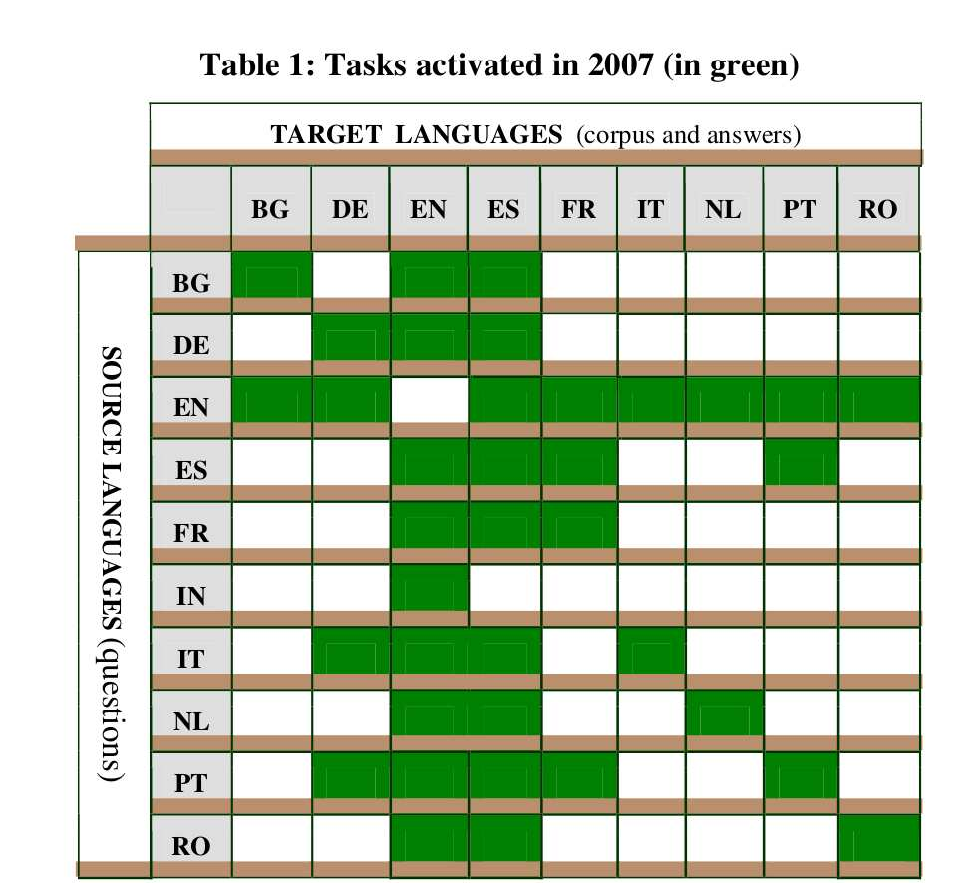
\includegraphics[scale=0.5]{graficos/clef07}
  \caption{Tareas activadas en la competencia Clef '07}
  \label{fig:tareas}
\end{figure}

El corpus de datos propuesto consiste en dos corpora distintos: una serie de de recopilados específicamente por los organizadores de la competencia y utilizado con frecuencia en competencias anteriores y, por otro lado, snapshots de las wikipedias en diferentes idiomas con límite en Diciembre de 2006.

Para nuestro proyecto utilizamos las preguntas y los datos de evaluación de los ejercicios monolingües es-es (español-español) y pt-pt (portugués-portugués) implementando como corpus de datos solo las wikipedias.

Los datos de los ejercicios constan de dos archivos: un archivo con 200 preguntas agrupadas por temas y otro archivo con diferentes traducciones de la pregunta, una respuesta goldstandard con soporte textual y el id del documento de soporte para el idioma target (del corpus).

Por otro lado, en la guía de ingreso a la competencia\cite{GuidelineClef07} se proveen links para descargar los snapshots de wikipedia sugeridos. Se ofrece una versión de wikipedia en inglés preprocesada de Noviembre de 2006 \footnote{\url{http://ilps.science.uva.nl/WikiXML/}}, dos opciones para descargar wikipedia en español: una imagen estática en html de Noviembre de 2006 \footnote{\url{http://static.wikipedia.org/downloads/November_2006/es/}} y un dump xml de Diciembre de 2006 \footnote{\url{http://download.wikimedia.org/images/archive/eswiki/20061202/pages-articles.xml.bz2}} y también X opciones de portugués.
%TODO: X

La guía aclara que, bajo responsabilidad de los participantes, se puede usar
cualquier otra versión de Wikipedia, siempre y cuando sea anterior a noviembre / diciembre de 2006.
Además, se pide que las respuestas sean tomadas de ``entradas reales'' o artículos de wikipedia y
no de otros documentos (imágenes, discusión, categoría, template, histórico de revisiones, datos de usuario y páginas con meta información).

Los links a páginas de wikipedia en español y en portugués no estaban más disponibles (ambos respondieron 404), mientras que el formato preprocesado pedido para el inglés resultaba realmente complejo de instalar y parecía una linea muerta. Por estos motivos, seguimos la sugerencia sobre el uso responsable de otras wikipedias y utilizamos las siguientes snapshots de Wikidumps\footnote{Ver \url{http://dumps.wikimedia.org/} y \url{http://en.wikipedia.org/wiki/Wikipedia:Database_download\#Other_languages}}. En la tabla \ref{table:wikipedias} pueden verse las diferentes wikipedias que procesamos durante el trabajo.

\begin{center}
\begin{table}
\begin{tabular}{ | l | l | l |}
    \hline
    Idioma & Fecha & Tamaño  \\ \hline
    Español & 5 de Julio de 2006 & 558M  \\ \hline
    Portugués & 1 de Febrero de 2007 & 776M   \\ \hline
    Inglés Simple & 4 de Julio de 2006 & 26M  \\ \hline
    Inglés & 4 de Noviembre de 2006 & 7,6G    \\ \hline
    Español & 26 de Enero de 2007 & 902M    \\ \hline
    Español & 14 de Junio de 2013 & 7,3G    \\ \hline
    Inglés Simple & 24 de Julio de 2013 & 406M    \\ \hline
\end{tabular}
\caption{Snapshots procesados con fechas y tamaños}
\label{table:wikipedias}
\end{table}
\end{center}

Utilizando la información disponible en los archivos de respuestas esperadas, discriminamos las preguntas con respuestas con soporte de wikipedia, las soportadas por el corpora de noticias de la organización y las que no tienen respuesta (NIL) (Ver table \ref{table:preguntas-por-respuesta}).

\begin{center}
\begin{table}
\begin{tabular}{| l | l | l | l | l |}
\hline
Idioma & Wiki & News & NIL & Total \\ \hline
es & 155 & 37 & 8 & 200 \\ \hline
pt & 130 & 59 & 11 & 200 \\ \hline
\end{tabular}
\caption{Total de preguntas con respuesta en Wikipedia, en otras fuentes y sin respuesta}
\label{table:preguntas-por-respuesta}
\end{table}
\end{center}


\subsection{Análisis de las preguntas}

Las 200 preguntas del test set están agrupadas por tema, y cada tema tiene de una a cuatro preguntas. Los temas pueden ser entidades nombradas, evento o también categorías como objetos, fenómenos naturales, etc (por ejemplo: Bush, Juegos Olímpicos, notebooks, huracanes, etc).
Los temas no están dados en el set de test, pero pueden ser inferidos del primer par pregunta respuesta. La relación del tema con el grupo de preguntas respetaba las siguiente condiciones:

\begin{itemize}
\item El tema es nombrado en la primer pregunta o bien en la primera respuesta.
\item Las siguientes preguntas pueden contener co-referencias al tema expresado en el primer par pregunta/respuesta
\end{itemize}


Para ilustrar el punto consideremos el primer grupo de preguntas para el ejercicio de español es:
\begin{itemize}
\item ¿En qué colegio estudia Harry Potter?
\item ¿Cuál es el lema del colegio?
\item ¿En qué casas está dividido?
\item ¿Quién es el director del colegio?
\end{itemize}


Como ya mencionamos, algunas preguntas podían no tener respuesta en la colección de documentos, y en ese caso la respuesta exacta era “NIL” y la justificación y el docid vacíos. La organización definió como criterio de inexistencia de la respuesta que ni los asesores humanos ni los demás sistemas participantes pudieran encontrar alguna.

En lo que respecta a los tipos de pregunta, el ejercicio considerara tres categorías: Factoid, Definition y Closed List.

\begin{center}
\begin{table}
\begin{tabular}{| l |  p {12cm} |}
\hline
Tipo & Descripción  \\ \hline
FACTOID & preguntas fácticas, preguntando el nombre de una persona, un lugar, la medida de algo, el día en que algo ocurrió, etc. \\ \hline
DEFINITION & preguntas como Qué/ Quién es X? \\ \hline
CLOSED LIST & questions that require one answer containing a determined number of items, e.g \\ \hline
\end{tabular}
\caption{Definición de los tipos de pregunta}
\label{table:question-type-definition}
\end{table}
\end{center}

Todos los tipos de pregunta podían contener restricciones temporales, i. e: una especificación temporal proveyendo importante información para devolver una respuesta correcta. Por ejemplo: \newline
Q: Who was the Chancellor of Germany from 1974 to 1982? \newline
A: Helmut Schmidt.\newline
Q: Which book was published by George Orwell in 1945?\newline
A: Animal Farm.\newline
Q: Which organization did Shimon Perez chair after Isaac Rabin’s death?\newline
A: Labour Party Central Committee.\newline


%Los calculos propios coinciden con el análisis presentado en \cite{OverviewClef07} en la siguiente discriminación del total de preguntas en función de las categorías recién señaladas:
\begin{center}
\begin{table}[H]
\centering
\begin{tabular}{| l | l | l | l | l | l |}
\hline
Subset & Idioma & Factoid & Definition & List & Total \\ \hline
\multirow{2}{*}{Todo} & es & 158 & 32 & 10 & 200 \\ \cline{2-6}
 & pt & 159 & 31 & 10 & 200 \\ \hline
 \multirow{2}{*}{Wiki} & es & 122 & 24 & 9 & 155 \\ \cline{2-6}
 & pt & 104 & 18 & 8 & 130 \\ \hline
\end{tabular}
\caption{Totales por tipo de pregunta}
\label{table:totals-type-question}
\end{table}
\end{center}

Los tipos de preguntas disponen a su vez de subtipos. Las preguntas factoid disponen de 8 subtipos, las de definiciones y listas tienen 4.
Se consideraron los siguiente 8 tipos de Factoids:

\begin{center}
\begin{table}[H]
\centering
\begin{tabular}{| l | p{12cm}|}
\hline
Tipo & Ejemplo \\ \hline
PERSON &  Q: Who was called the \dq{Iron-Chancellor}? \newline A: Otto von Bismarck. \\ \hline
LOCATION & Q: Which town was Wolfgang Amadeus Mozart born in? \newline A: Salzburg. \\ \hline
ORGANIZATION & Q: What party does Tony Blair belong to? \newline A: Labour Party.\\ \hline
MEASURE &Q: How high is Kanchenjunga?\newline A: 8598m. \\ \hline
COUNT & Q: How many people died during the Terror of Pol Pot? \newline A: 1 million.\\ \hline
OBJECT & Q What does magma consist of?\newline A: Molten rock.\\ \hline
TIME & Q: What year was Martin Luther King murdered?\newline A: 1968.\\ \hline
OTHER & i.e. todo lo que no encaja en las categorías anteriores.\newline Q: Which treaty was signed in 1979? \newline
A: Israel-Egyptian peace treaty.\\ \hline
\end{tabular}
\caption{Tipos de respuesta esperada para preguntas Factoid}
\label{table:type-factoid}
\end{table}
\end{center}

Las preguntas de tipo LIST consisten en enumeraciones de 4 subtipos posibles: PERSON, LOCATION, ORGANIZATION y OTHER.
Por ejemplo:\newline
Q: Name all the airports in London, England. \newline
A: Gatwick, Stansted, Heathrow, Luton and City.

Como solo una fuente estaba permitida, los items debían aparecer en secuencia, uno después del otro, en un solo documento de la colección.
Las preguntas de tipo DEFINITION tienen también estos mismos cuatro subtipos, pero con una semántica ligeramente diferente. En la tabla \ref{table:definition-questions} presentamos ejemplos y la definición inferida sobre estos tipos.

Por su parte, en la table \ref{table:tipo-general} puede verse una clasificación general de preguntas por tipo y por subtipo para los ejercicios de español y de portugués.

\begin{center}
\begin{table}[H]
\centering
\begin{tabular}{| l | p{12cm}|}
\hline
Tipo & Descripción y ejemplo \\ \hline
PERSON & i.e. preguntas sobre el rol, el trabajo o información importante de alguien \newline
 Q: Who is Robert Altmann? \newline
 A: Film maker. \\ \hline
ORGANIZATION & i.e. preguntas sobre la misión, el nombre completo o información relevante sobre una organización \newline
 Q: What is the Knesset? \newline
 A: Parliament of Israel. \\ \hline
OBJECT & i.e. preguntas por la descripción o función de objetos \newline
Q: What is Atlantis? \newline
A: Space Shuttle. \\ \hline
OTHER & i.e. preguntas por descripciones de fenómenos naturales, tecnologías, procedimientos legales, etc. \newline
Q: What is Eurovision? \newline
A: Song contest. \\ \hline
\end{tabular}
\caption{Tipos de respuesta esperada para preguntas Definition}
\label{table:definition-questions}
\end{table}
\end{center}

\begin{center}
\begin{table}[H]
\centering
\begin{tabular}{| l | l | l | l | l | l |l |l|l|}
\hline
Tipo & pt & es & pt-factoid & es-factoid & pt-def & es-def & pt-list & es-list \\ \hline
COUNT & 21 & 22 & 21 & 22 & 0 & 0 & 0  & 0\\ \hline
OBJECT & 11 & 27 & 6  & 18 & 5 & 9 & 0  & 0\\ \hline
MEASURE & 15 & 20 & 15 & 20 & 0 & 0 & 0  & 0\\ \hline
PERSON & 33  & 35 & 21 & 24 & 9 & 8 & 3 & 3\\ \hline
TIME & 19 & 16 & 18 & 16 & 0 & 0 & 1 & 0\\ \hline
LOCATION & 33 & 18  & 30 & 18 & 0 & 0 & 3 & 0 \\ \hline
ORGANIZATION & 31 & 32 & 24 & 22 & 6 & 8 & 1 & 2\\ \hline
OTHER & 37 & 30 & 24 & 18 & 11 & 7 & 2 & 5 \\ \hline
Total & 200 & 200 & 159 & 158 & 31 & 32  & 10 & 10\\ \hline
\end{tabular}
\caption{Tipos de respuesta esperada en función de tipo de pregunta}
\label{table:tipo-general}
\end{table}
\end{center}


\section{Sistema}
\label{sec:sistema}

Nuestra implementación está basada en Qanus como framework o arquitectura de diseño de QA y en Freeling como proveedor de servicios de procesamiento de lenguaje multilingüe. Qanus (Question-Answering @ National University of Singapore) es un framework de question answering basado en information retrieval y también un sistema de QA funcional simple construido sobre este framework. El proyecto se actualizó por última vez en noviembre de 2012 y contiene herramientas actuales de nlp para inglés (el POS-tagger, el NER-tagger y el Question Classifier de Stanford) y también de information retrieval (índice de búsquedas lucene) bajo licencia de código abierto. El paquete cuenta con un framework (qanus), que cumple un rol equivalente a la arquitectura DeepQA en la organización del proyecto de IBM, y un sistema montado sobre este framework -QA-sys-, equivalente a Watson (Ver Figura ~\ref{fig:Quanus}).


\begin{figure}
  \centering
    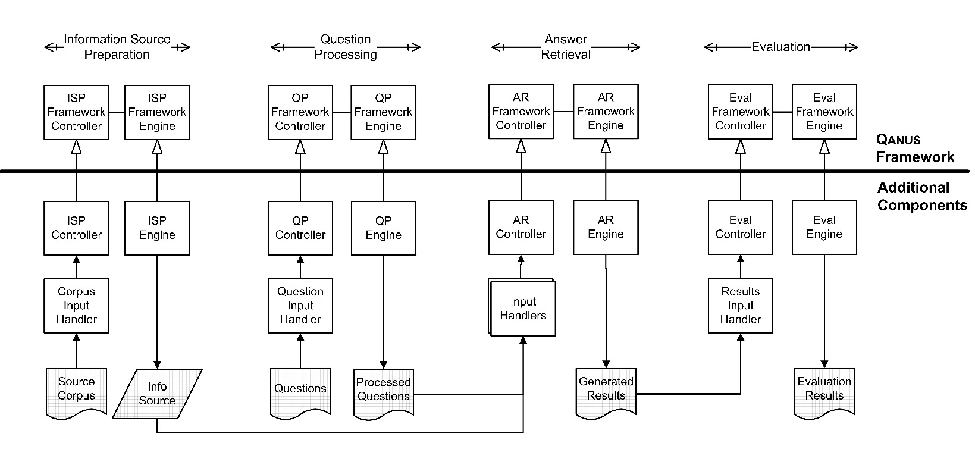
\includegraphics{graficos/Quanus}
  \caption{El framework Quanus y la implementación QA-sys}
  \label{fig:Quanus}
\end{figure}


La arquitectura de Qanus mantiene la estructura de pipeline típica similar a las reseñadas en la sección \allref{chap:estado-de-arte}.
Consta de los siguientes pasos: \newline

\textbf{Preparación de la fuente de información: } El primer step del pipeline es preprocesar las fuentes de información para un acceso optimizado en pasos posteriores del proceso. La implementación QA-sys incorpora una base de conocimiento en formato XML de aquaint a un índice de
búsquedas Lucene. En este paso se incorpora todo el conocimiento offline; bases de conocimiento dinámicas como la web se modelan en el pasos posteriores. \newline

\textbf{Análisis de la pregunta: } Este paso, igualmente genérico, permite la incorporación de
distintos componentes para anotar los tokens de la pregunta con datos
útiles para ser consumidos por el paso 3. Otro procesamiento a
realizar en este paso podría ser la generación de queries
entendibles por los distintos motores de almacenamientos de
información del paso 1. En particular, la implementación trae un
pos-tagger, un ner-tagger y un question classifier, todos de Stanford.
Hablaremos más de estos componentes más adelante. \newline

\textbf{Generación de respuestas: } En este paso se utiliza la información generada en la preparación
de la base de información y en el procesamiento de la pregunta para
generar una respuesta. También puede incorporarse accesos a la web y
validaciones de las respuestas candidatas. La implementación concreta
evalúa cada pasaje de los primeros n documentos retornados por Lucene
para la pregunta original con una serie de componentes ad-hoc de
distancia para adjudicar diferentes grados de confiabilidad a los
distintos pasajes. \newline


Además, se provee de un cuarto paso opcional (el sistema de QA está
completo con los tres pasos anteriores), para la fase de desarrollo y
de evaluación de la performance del sistema:\newline


\textbf{Evaluación: }Este paso está pensado para evaluar las respuestas generadas y
presentarlas de un modo conciso en la fase de desarrollo.
Básicamente, cruza las respuestas obtenidas contra unas respuestas
esperadas escritas a mano y presenta el total de respuestas dadas
correctamente.\newline

En esta sección de la tesis adoptamos el framework Qanus y adaptamos el sistema QA-sys para 1) incorporar Freeling como librería de herramientas de procesamiento del lenguaje permitiendo un funcionamiento multilenguaje, 2) trabajar sobre el corpus de datos y preguntas de los ejercicios de CLEF '07 de español y portugués descriptos en \allref{sec:ejercicio-de-clef} y, finalmente, 3) incorporamos y evaluamos diferentes mejoras tomadas de la reseña a la literatura científica del apartado anterior \allref{sec:literatura}.

\subsection{Implementación baseline}
\label{subsec:baseline}
El código está escrito en java y mantiene una interfaz común a
todos los pasos: un controller cuyas responsabilidades son cargar los
componentes y un engine que utiliza los componentes para leer el input,
procesarlo y grabar el resultado. La adaptabilidad del framework está
dada en la posibilidad de incorporar componentes respetando la interfaz
especificada para los mismos o bien, en modificar esta misma interfaz.

La implementación QA-sys está desarrollada para correr sobre
el tipo de datos de las evaluaciones Trec 2007.
Brevemente, la implementación realiza las siguientes tareas:
En el primer paso, incorpora los XML en el formato XML Aquaint propuesto por la competencia a un índice Lucene, en
el segundo paso anota la pregunta con POS tags, NERs y
clasifica el tipo de respuesta con un clasificador entrenado y luego,
en el tercer paso se busca la pregunta sobre el índice lucene y se
retorna una lista con n documentos rankeados. Estos documentos se
subdividen en pasajes. Luego se aplican diferente algoritmos ad-hoc
dependiendo del tipo de respuesta esperada. \ Por ejemplo, si la
respuesta es un nombre de persona, se ejecuta NER sobre los diferentes
pasajes buscando nombres candidatos, si el tipo esperado es una fecha,
se utilizan expresiones regulares escritas a mano, etc. Finalmente, los
pasajes candidatos se evalúan utilizando heurísticas de proximidad
de los candidatos a la pregunta inicial. Para esto se utilizan
diferentes Scorers que rankean los pasajes según diferentes
características (features) y luego se selecciona alguna priorizando
algunas características sobre otras, dependiendo también del tipo
de respuesta esperada. Por último, el evaluador de resultados mide la
exactitud (\textit{accuracy}): total de respuestas correctas sobre
total de preguntas.

QA-sys funciona sólo sobre preguntas del tipo
factoid y, a modo de comparación, el mejor sistema según la Trec
2007, el LymbaPA07 obtuvo un grado de exactitud del 0.706 y el décimo
(Quanta) obtuvo 0.206, mientras que QA-sys logra el 0.119 disponiendo de una implementación sumamente simple.

En las siguientes secciones de la tesis describiremos la implementación de nuestro sistema de question answering tomando como base los tres pasos principales del pipeline de QA-sys.

\subsubsection{Base de conocimiento}

El módulo de procesamiento de la base de información de la implementación QA-sys está desarrollada para correr sobre el tipo de datos de las evaluaciones Trec 2007, un formato XML conocido como ``Aquaint". Por otro lado, el mismo framework esta atado al procesador de XMLs SAX, una entre varias implementaciones disponibles en el entorno de java. En nuestra adaptación, incorporamos la librería gwtwiki\footnote{Java Wikipedia API (Bliki engine): \url{http://code.google.com/p/gwtwiki/}} para procesar los xml dumps de wikipedia. Como esta librería no utiliza SAX, nos vimos obligados a modificar el framework.

En este proceso descartamos artículos mal formados y entradas representado imágenes o discusiones, tal como se sugiere en la guía.
Los artículos se indexan en índices Lucene como documentos con los siguiente campos: \emph{id, title, body y all}.
La tabla \ref{table:creacion-indices} muestra algunos datos del proceso de generación de índices.

Las categorías filtradas contienen artículos con alguno de los siguientes prefijos en el título: WP, wp, Biografías, Wikipedia, Wikiproyecto, Imagen, Plantilla, MediaWiki, Template, Category, Help, Image, Ayuda, Portal, Ajuda, Categoria, Categoría, Imagem, Predefinição.


\begin{table}
\centering
\begin{center}
\begin{tabular}{| l | l | l | l | l | l| l|}
\hline
Wikipedia & \# Entradas & Nulas & Redirects & Filtradas & Validas \\ \hline
simple-06 & 18273 & 22 &  3452 & 5241 & 9558  \\ \hline
es-06 & 233750 & 52 & 62805 & 34947 & 135946 \\ \hline
pt-07 & 498039 & 80 & 210983 & 43390 & 243586 \\ \hline
simple-13 & 180067 & 8 & 35600 & 41902 & 102557\\ \hline
\end{tabular}
\caption{Wikipedias: cantidad de entradas válidas e inválidas}
\label{table:creacion-indices}
\end{center}
\end{table}

\subsubsection{Anotado de la pregunta}

El módulo original de QA-sys de procesamiento de la pregunta espera preguntas en el formato Aquaint definido por Trec, al igual que el tipo de datos esperado sobre el corpus en el paso anterior. Durante el procesamiento clasifica la pregunta, y ejecuta un POS tagger y un NER tagger, utilizando como librerías de procesamiento de lenguaje el POS-Tagger, el NER-Tagger y el Question Classifier de la Universidad de Stanford, disponibles solo para inglés, descriptas en \allref{sec:stanford-both} y \allref{sec:stanford-qc} respectivamente.

En nuestra adaptación incorporamos los módulos de POS y NERC multilingües de freeling. Con respecto a la clasificación de preguntas, ya mencionamos que no existen clasificadores para español y tampoco para el portugués. Frente a esta situación podríamos haber implementado clasificadores heurísticos basados en reglas escritas a mano. Esta implementación nos desviaba de nuestro proyecto, por lo que utilizando la disponibilidad de una traducción confiable al inglés de las preguntas en archivos de datos (debido a la activación de los ejercicios cross-lingual en-es y en-pt), decidimos utilizar el clasificador de Stanford sobre la traducción inglesa de la pregunta para clasificarlas en el idioma en cuestión.
La tabla \ref{table:qc-es-pt} presenta la distribución de las 200 preguntas para español y para portugués según las seis clases principales del esquema de Li \& Roth obtenida al clasificar las preguntas con el clasificador de Stanford.

\begin{table}
\centering
\begin{center}
\begin{tabular}{| l | l | l | }
\hline
Clase & \# Preguntas (es)  & \# Preguntas (pt)\\ \hline
HUM &  62 & 53 \\ \hline
NUM &  53 & 52\\ \hline
ENTY &  34 & 28\\ \hline
DESC &  25 & 30\\ \hline
LOC &  24 & 36\\ \hline
ABBR &  2 & 1\\ \hline
\end{tabular}
\caption{Distribución por clases de las preguntas para español y portugués}
\label{table:qc-es-pt}
\end{center}
\end{table}


Al finalizar el paso del anotado de la pregunta, las preguntas tienen asociado su tipo, las distintas entidades nombradas, el análisis gramatical y las qwords. Dejamos la generación de queries para el paso posterior ya que así es como estaba implementado en el sistema original.

\subsubsection{Generación de Respuestas}

Como baseline de desarrollo y pruebas, adaptamos los algoritmos de Qanus. En esta subsección vamos a describir esta implementación con detalle, mencionando los cambios más importantes que realizamos para adaptarla a la tarea elegida. En las siguientes comentaremos diferentes modificaciones y algoritmia agregada. El proceso de qanus para la generación de respuestas puede estructurarse así:
\begin{enumerate}
  \item Filtrado de preguntas
  \item Generación de Queries
  \item Information Retrieval
  \item Extracción y rankeo de oraciones
  \item POS tagging de las mejores oraciones
  \item Heurísticas de AR basadas en el QC
\end{enumerate}

En el primer paso, se descartan todas las preguntas cuyo tipo no sea \textit{factoid}. Esto, en principio, dejaría afuera a 32 preguntas de tipo \textit{definition} y 10 de tipo \textit{list} para el ejercicio en español (24 y 9, respectivamente, considerando solamente las que como goldstandard answer tienen datos de wikipedia) y 31 de tipo \textit{definition} y 10 de tipo \textit{list} para el portugués (18 y 8, respectivamente, considerando las de wikipedia).

En en segundo paso, la generación de queries, el sistema baseline utiliza 2 algoritmos diferentes según el qtype inferido por el clasificador de preguntas. El primer caso es especifico para la clase fina \sq{HUM:ind} y consta de tres tipos de expresiones regulares escritas a mano y en inglés que matchean contra preguntas de la forma: \dq{Who (is|was) (the)+ NN ... NN?} (NN significa, acá, sustantivo). Por ejemplo: \dq{Who is the CEO of Microsoft?}. También se considera aquí preguntas con la forma \dq{Who VERBO ...?}. Para este tipo de expresiones, el algoritmo específico extrae los sustantivos y los verbos de la pregunta para generar la query. Eliminamos este caso ya que su dependencia del idioma volvía el procedimiento obsoleto para un sistema con soporte multilenguaje.

Por su parte, si el tipo de la pregunta no es \sq{HUM:ind}, el algoritmo general de generación de queries espera, además de la pregunta propiamente dicha, un campo asociado a la pregunta, \sq{target}, aparentemente definido en la competencia TREC para la que está escrito. El campo \sq{target} es utilizado por mucha de la algoritmia que vendrá. Dejaremos en suspenso con qué poblamos ese dato hasta más adelante. Un uso posible es asociarlo el \sq{tópico} del grupo de preguntas de los ejercicios de la competencia. Más adelante veremos qué contenido le cargamos.


El método default FormQuery genera una query que contiene, sin repetir, todas las palabras no-stopwords del campo target y todos los sustantivos, verbos y adjetivos de la pregunta completa según el pos tagger de stanford. Nosotros adaptamos este método para funcionar con las etiquetas de Freeling y utilizamos este mecanismo de generación de queries como baseline.

En el tercer paso, a partir de la query generada se hace un pedido al índice lucene y se obtiene una lista de documentos. En el cuarto paso, los documentos son divididos en sus oraciones de manera indiscriminada, es decir: las oraciones no heredan posición de acuerdo al ranking de los documentos a los que pertenecían.

Las oraciones se evalúan mediante el peso ponderado de diferentes features que consideran la query generada y la oración, generando un nuevo orden entre ellas, basado en su \textit{score}. El score es un valor real entre 0 y 1, que sigue la siguiente fórmula:

\medskip

$PassageScore = (0.9)*CoverageScore + (0.05)*FreqScore+ (0.05)*ProxScore;$

\medskip
Los scorers $coverage$, $freq$ y $prox$ son diferentes métricas de evaluación de oraciones, cuya imagen es una valor real entre 0 y 1. En la tabla \ref{table:scorers} se hace una presentación general de los Scorers y a continuación explicamos los algoritmos de $Prox$ y $Span$ ya que no son triviales ($Span$ aún no ha sido utilizado pero lo será en breve).

\begin{center}
\begin{table}
\begin{tabular}{| l | l | p {8cm} |}
\hline
Abreviatura & Nombre &  Descripción\\ \hline
Freq & Frequencia & Computa la cantidad de veces que los tokens de la query ocurren en la oración. Esta suma se divide por la cantidad de tokens de la oración, dando un valor entre 0 y 1. \\ \hline
Coverage & Cobertura &  Computa cuantos tokens de la query aparecen al
menos una vez en la oración, y divide esta suma por el total de tokens
de la \textit{query}.\\ \hline
Prox & Proximidad &  Computa la distancia entre dos strings en un tercero. Ver aparte.   \\ \hline
Span & Distancia entre tokens & Computa la distancia media entre términos de la query en la oración. Ver aparte. \\ \hline
\end{tabular}
\caption{Scorers de Qanus}
\label{table:scorers}
\end{table}
\end{center}

$Prox$ toma dos strings a buscar en un tercero. Busca ambos en el tercero y computa la distancia en tokens entre ellos.
Esta distancia se calcula como la distancia entre el centro de ambos strings.
Por ejemplo, para los strings de búsqueda \dq{Argentina es un país americano} y \dq{independizado en 1810} sobre el texto \dq{Argentina es un país americano, originalmente una colonia española, independizado en 1810} se considera la distancia entre \sq{un} y \sq{en} (por ser los tokens \sq{intermedios} de ambos strings
de búsqueda. La distancia entre ambos, en el tercer string, es 7 (la cantidad de tokens entre ellos). Esta distancia se divide por la longitud en tokens del string en el que se buscan (12), dando un resultado de 0.58. Un score cercano a 1 denota que los dos string están cercanos uno al otro en el tercer string.
%TODO: no anda en el original no?? Porque dice que tiene que recibir 2 elementos y recibe siempre solo 1

Por su parte, $Span$ tiene un concepto similar, pero funciona sobre un solo string de búsqueda, considerando sus tokens. Los distintos tokens buscados ocurren en ciertas posiciones. $Span$ considera la distancia entre las posiciones de los tokens más distantes, dividiendo el total de tokens encontrados por este valor.
Un score cercano a 1 significa que los términos del string buscado están cerca en el string en el que se buscan.
Por ejemplo, suponiendo los siguientes matchs de tokens (denotados por una X): \newline
..... X ..... X ..... X ...... \newline
......a ...... b ...... c ...... \newline

El score de $Span$ estaría dado por \#total de tokens encontrados /  {\textbar}posición de c- posición de a{\textbar}.



\medskip

En el quinto paso se seleccionan las 40 oraciones mejor rankeadas según este score y se les aplica pos tagging.

Finalmente, el sexto paso ejecuta diferentes heurísticas de extracción de respuestas en base al tipo de pregunta generador por el clasificador en el paso anterior.
Define diferentes heurísticas para los siguientes casos: ABBR:exp, ABBR:abb, HUM:gr,\newline

\textbf{Caso ABBR:exp}\newline

Si el tipo de respuesta esperada es ABBR:exp (expansión de una abreviación), entonces el algoritmo de extracción es el siguiente: primero, se extraen las entidades nombradas de tipo \sq{Organización} desde la pregunta. Con ellas, se generan regex de expansión de esa abreviación. Por ejemplo, para la abreviación \dq{IGFA} se genera la regex $[I]+[A-Za-z0-9]+ [G]+[A-Za-z0-9]+ [F]+[A-Za-z0-9]+ [A]+[A-Za-z0-9]+ $. En términos coloquiales, esta regex sirve para buscar en fragmentos de texto por expresiones con la forma I... G... F... A.... Por cada una de las 40 oraciones mejor rankeadas, el proceso busca por ocurrencias de ese patrón. Finalmente, no realiza ningún trabajo posterior y devuelve la primera encontrada. \newline

\textbf{Caso ABBR:abb}\newline

Este tipo de respuesta esperada representa el pedido de una contracción de una abreviación, la inversa de la anterior. Por ejemplo, \dq{¿Con qué siglas se conoce a la corporación \sq{International Business Machines}?} (IBM). El caso no tiene código: \textit{// Abbreviations : Contractions -> What can we do?} \newline

\textbf{Caso HUM:gr y ENTY:cremat} \newline

El tipo HUM:gr refiere a grupos humanos, como compañías u organizaciones, mientras que ENTY:cremat refiere a entidades de creación humana (como libros, inventos, discos, etc).
Para este caso, el proceso consiste en extraer nombres propios (proper nouns, NNPs) de todas las oraciones rankeadas (se asume que nombres propios consecutivos representan un solo nombre propio, por ejemplo Tiger/NNP, Woods/NNP forman un nombre propio solo). Sobre estos resultados se ejecutan filtros basados en diccionarios. En concreto, se eliminan los siguientes términos: \{Monday, Tuesday, Wednesday, Thursday, Friday, Saturday, Sunday\}, \{January, February, March, April, May, June, July, August, September, October, November, December\}, \{us, uk, france, england, cuba, japan, u.s, america\}. Para cada respuesta candidata que pasó el filtro, se rankean de acuerdo a diferentes scores basados los comparadores $coverage$, $freq$ y $prox$.
La fórmula de ponderación utilizada es la siguiente: \\

$TotalScore = (0.55 * CoverageScore) + (0.2 * SentenceScore)	+ (0.1 * ProximityScore) + (0.15 * RepeatedTermScore)$

Donde $CoverageScore$ es el cubrimiento del \sq{$target$} de la pregunta en la oración de soporte de la respuesta, $ProximityScore$ mide la distancia entre el \sq{target} de la pregunta y la respuesta candidata en el contexto de la oración de soporte, $SentenceScore$ considera la posición de la oración en el ranking de las 40 oraciones y $RepeatedTermScore$ es una penalización (su valor es negativo) si la respuesta candidata tiene tokens en común con el \sq{target} de la pregunta. En la adaptación inicial eliminamos este filtrado por diccionarios ya que depende del idioma. \newline

\textbf{Caso HUM:ind} \newline

El tipo HUM:ind son preguntas que refieren a un individuo humano. El algoritmo en este caso intenta generar, para ciertos patrones, el subject (como en los casos especiales de generación de queries). Eliminamos este caso ya que se basa en expresiones regulares específicas por idioma. Luego, para cada oración se extraen las entidades nombradas de tipo \sq{PERSON}. Para cada respuesta candidata, se evalúan distintos features para generar un score general:

$TotalScore = (0.5 * CoverageScoreTarget)+ (0.25 * CoverageScoreSubject) + (0.35 * SentenceScore) +
					 (0.25 * ProximityScore)	+ (0.1 * RepeatedTermScore) + (0.5 * IsPronoun)$\newline

Donde los scores representan lo siguiente:
\begin{itemize}
  \item CoverageScoreTarget: cuántos tokens del \sq{target} aparecen en la oración fuente de la respuesta candidata
  \item CoverageScoreSubject: cuántos tokens del subject aparece en la oración fuente de la respuesta candidata (si era el caso, cero si no)
  \item SentenceScore: puntaje derivado de la posición de la oración-fuente en el ranking de oraciones
  \item ProximityScore: cuán cerca están la query utilizada como input del módulo de information retrieval (sin stop-words) y la respuesta candidata en el contexto de la oración de la que se extrajo la respuesta candidata.
  \item RepeatedTermScore: penalización (negativo). Coverage entre el \sq{target} y la respuesta candidata
  \item IsPronoun: Penaliza si la respuesta candidata contienen pronombres. En concreto, verifica si algún token pertenece a la lista \{it, we, he, she, they, our, their\}.
\end{itemize}

En base a este score, se devuelve la respuesta candidata con puntaje más alto. \newline

\textbf{Caso HUM general} \newline

Este caso contempla todos los tipos de respuestas esperadas de clase HUM (humano) que no son gr ni ind (estos son dos casos: título y descripción). En este caso, se toma el primer nombre propio de la oración mejor rankeada y se utiliza eso como respuesta. \newline

\textbf{Caso LOC general} \newline

La clase LOC (location o locación) incluye preguntas que refieren a lugares.  En este caso, se extraen todas las entidades nombradas de tipo \sq{LOCATION} de las oraciones rankeadas y se las evalúa según el siguiente scoring:

$TotalScore = (0.6 * CoverageScore) + (0.1 * SentenceScore) + (0.2 * ProximityScore)	+ (0.5 * SanityScore) + (0.3 * RepeatedTermScore)$ \newline

Estos scores son:
Donde los scores representan lo siguiente:
\begin{itemize}
  \item CoverageScore: cuántos tokens del \sq{target} aparecen en la oración fuente de la respuesta candidata
  \item SentenceScore: puntaje derivado de la posición de la oración-fuente en el ranking de oraciones
  \item ProximityScore: cuán cerca están la query utilizada como input del módulo de information retrieval (sin stop-words) y la respuesta candidata en el contexto de la oración de la que se extrajo la respuesta candidata.
  \item RepeatedTermScore: penalización (negativo). Coverage entre el \sq{target} y la respuesta candidata.
  \item SanityScore: es un placeholder para implementar código comentado. En el código que encontramos, vale 1 (constante).
\end{itemize}


\textbf{Caso NUM:date} \newline

Este tipo de respuesta esperada representa una fecha. El algoritmo verifica la ocurrencia del término \sq{year} en la pregunta. Si la pregunta contiene el término, genera un patrón para buscar años (una expresión regular) y devuelve el primero que encuentra. En caso contrario, devuelve el título del primer documento encontrado (ya que el módulo está implementado para responder preguntas de TREC y los documentos son artículos cuyos títulos tienen, en general, fechas). Como oración de justificación, toma la primer oración del documento.

En nuestra adaptación, recaímos en el caso general para la clase NUM, especificándole a Freeling que solo considere fechas (ver tres títulos más abajo).

\textbf{Caso NUM:period} \newline

Este tipo de respuesta esperada representa un periodo de tiempo. El código busca en la pregunta por el patrón \dq{How old (is|was) NNP{1,}?} (donde \dq{NNP{1,}} significa uno o más nombres propios seguidos) y se queda con la secuencia de nombres propios como \textit{subject}.
Si logra detectarse este subject, se busca en las oraciones rankeadas por números y por números seguidos de los tokens \dq{years old}. Luego se rankean estos números según la siguiente fórmula:\newline

$TotalScore = (0.8 * ProximityScore) + (0.2 * SentenceRankScore)$ \newline

Donde ProximityScore mide la distancia entre el número y el subject en el contexto de la oración de la que se extrajo el número y SentenceRankScore representa el ranking de la oración dentro de las 40 oraciones.

Si la detección del subject o de los números es infructuosa, se recae en una estrategia general para la clase NUM, que consiste en buscar el primer número encontrado por el pos tagger (hardcodeado para los tags usados por Stanford como CD) y devolverlo.

En nuestra adaptación, eliminamos el caso del subject porque dependía del idioma y recaímos en el el caso general. \newline

\textbf{Caso NUM:count} \newline

Este tipo de respuesta esperada representa un número. El algoritmo busca por el patrón \dq{How many ...?} intentado extraer el \textit{subject}, por ejemplo, para la pregunta \dq{How many miners...?} el subject es \dq{miners}. Con este subject, realiza exactamente los mismos pasos que el caso inmediatamente anterior y nosotros realizamos la misma adaptación, esta vez especificando que los números buscados no sean fechas. \newline


\textbf{Caso NUM general} \newline

Considera los casos numéricos no contemplados en los tres casos anteriores. El algoritmo ejecutado consiste en encontrar el primer set continuo de tokens taggeados como \sq{CD} (números) por el POS tagger de Stanford. En nuestra adaptación a Freeling, pudimos mejorar esto separado dos tipos de números: los referidos a fechas y los referidos a cantidades. En el caso general, se busca cualquier tipo de números. Sin embargo, como especificamos en los títulos inmediatamente anteriores, para ciertos casos especificamos o bien fechas, o bien cantidades. \newline

\textbf{Caso ENTY general} \newline

El caso de entidades general incluye todas las subclases que no son \sq{cremat}. El algoritmo implementado es el mismo que para el caso de \sq{HUM} general, este es: tomar el primer nombre propio de la oración mejor rankeada y utilizarlo como respuesta.
Busca cualquier sustantivo y retorna el primero que encuentra.  \newline

\textbf{Otro caso} \newline

Se implementa el mismo algoritmo que el caso anterior. \newline


\subsection{Modificaciones}
\label{subsec:modificaciones}

Además de los cambios realizados para convertir al baseline de qanus en un sistema multilingüe basado en la librería freeling, realizamos algunos agregados mínimos a la lógica. En esta sección describiremos diferentes modificaciones realizadas y en la siguiente veremos la evaluación comparativa entre la performance del sistema baseline y las modificaciones en las diferentes tareas que realizan los submódulos.

\subsubsection{Inferencia del tópico del grupo de preguntas}
\label{subsubsec:entidad-de-grupo}

Como vimos anteriormente, los ejercicios consisten en preguntas agrupadas en torno a tópicos con entre 1 y 4 preguntas. Este tópico está disponible en los archivos de datos, pero se esperaba que en la competencia no se utilicen. Los temas pueden ser entidades nombradas, evento o también categorías como objetos, fenómenos naturales, etc. Por ejemplo, estos son algunos de los primeros temas del test set de español: \sq{Colegio de Harry Potter}, \sq{Pez Espada}, \sq{Amintore Fanfani}, \sq{Revolución de Terciopelo}. Según mencionamos anteriormente, el tema del grupo de preguntas respeta las siguiente condiciones:

\begin{itemize}
\item El tema es nombrado en la primer pregunta o bien en la primera respuesta.
\item Las siguientes preguntas pueden contener co-referencias al tema expresado en el primer par pregunta/respuesta
\end{itemize}

Aprovechamos el campo \sq{target} del sistema baseline para incorporar este tópico al flujo de procesamiento, ya que su funcionalidad es la esperada para este input.
Finalmente, evaluamos diferentes contenidos para este valor. A modo de testeo, utilizamos, aún cuando en la competencia no estaba permitido, el tópico real del grupo según el test set. Por otro lado, implementamos otros tres métodos para generar el tema, siempre basándonos en la pregunta. Hicimos esto por considerar que las respuestas, probablemente, sean erróneas. Dado que no podemos saberlo, apoyar algoritmia sobre el supuesto de que estén bien sería contraproducente para el caso general. Así, implementamos: un método en el cual se agregan solo las entidades nombradas, los números y las fechas de la pregunta, otro en el que se agregan solo los sustantivos y, finalmente, otra en la que se agregan ambos. Si el método elegido no funciona, se utiliza la pregunta sin stop words ni qwords. En todos los casos, nos referimos a la primer pregunta del grupo.

En concreto, esto se reduce a cuatro casos de código, que en la sección de experimentación llamaremos: \textbf{1) Tema Test}, cuando utilizamos el tema explícito de los datos de testing, (\textbf{2) Tema NERS}), \textbf{3) Tema sustantivos} y \textbf{4) Tema híbrido}.

\subsubsection{Generación de queries}

Para la extracción de queries utilizamos, como primer método y baseline de evaluación, el implementado por qanus. La query generada contiene, sin repetir, todas las palabras no-stopwords del campo target y todos los sustantivos, verbos y adjetivos de la pregunta completa contra el campo $ALL$. En la evaluación llamaremos a este método \textbf{baseline}. Le agregamos, además, números y fechas al final. Implementamos un segundo método, aprovechando el conocimiento de la estructura de datos del índice, que consiste en agregarle a esta misma query un caso, si el tema no es vacío, en el que se busca por este tema en el título de los artículos, con un peso virtualmente infinito frente al resto de la query.

Es decir, la query generada por el método dos tiene la forma siguiente: \textit{(TITLE: target)$^n$ OR \textbf{query baseline}}. En concreto, utilizamos $n=5$. En la evaluación llamaremos a este método \textbf{improved baseline}.

Finalmente, implementamos la heurística propuesta por los papers \cite{QA1} y \cite{QA3}, que, recordamos, consiste en 8 reglas para agregar, en orden, a la query:

\begin{enumerate}
\item Todas las palabras no stop words entre comillas
\item Todas las entidades nombradas reconocidas
\item Todas las construcciones nominales con sus adjetivos
\item Todas las demás construcciones nominales
\item Todos los sustantivos con sus adjetivos
\item Todos los demás sustantivos
\item Todos los verbos
\item El \sq{focus} de la pregunta
\end{enumerate}

Dado que no implementamos ningún algoritmo de extracción de \textit{focus}, el último ítem fue reemplazado por el tema de la pregunta, si existiera.  En la evaluación llamaremos a este método \textbf{lasso}, por el nombre del sistema en el que fue implementado por primera vez. Además, agregamos números y fechas también, como en el baseline. En realidad, detectores de entidades distintos de freeling suelen incorporar los números como entidades nombradas, por lo que no salimos de la propuesta de lasso.

\subsubsection{Generación de respuestas}

Con respecto a la generación de respuestas, incorporamos solamente distintos scorers nuevos para rankear los pasajes y no modificamos los mecanismos baseline de extracción de respuestas a partir de pasajes más allá de lo explicado en la sección anterior.
Los nuevos features incorporados son:

\begin{itemize}
\item LengthScore : Contempla la longitud del pasaje, priorizando oraciones cortas pero no demasiado cortas. Este score trata de evitar problemas vinculados con mala redacción en los documentos que generaban pasajes enormes y sin sentido para las librerías.
\item QVerbScore: Contempla la presencia de verbos de la pregunta en el pasaje candidato.
\item QNounScore: Contempla la presencia de sustantivos de la pregunta en el pasaje candidato.
\item QNERScore: Contempla la presencia de las entidades nombradas de la pregunta en el pasaje candidato.
\end{itemize}

Todos están normalizados (son reales entre 0 y 1 inclusive). El objetivo de los últimos tres fue distinguir, dentro de lo que es el score de cobertura, la presencia de términos de importancia destacada dentro del pasaje.


Con estos cuatro scores nuevos, implementamos tres métodos de rankeo de pasajes. El primero es el \textbf{baseline} y su formula de rankeo es la siguiente: \newline

$PassageScore_{bl} = (0.9)*CoverageScore + (0.05)*FreqScore+ (0.05)*ProxScore;$ \newline

El segundo método y tercer método utilizan este score y se definen como sigue:\newline

$PassageScore_2 =  PassageScore_{bl} * 0.4 + QNERScore * 0.2 + QVerbScore*0.15	+ QNounScore * 0.25 $\newline

$PassageScore_3 =  PassageScore_{bl} * 0.4 + LengthScore * 0.15 + QNERScore * 0.1 + QVerbScore*0.1	+ QNounScore * 0.25 $\newline


\subsection{Experimentación}
\label{sec:eval}

Hicimos corridas con todas las combinaciones recién expuestas y, además, variamos la cantidad de documentos retornados por lucene (50 en el sistema baseline) y la cantidad de pasajes extraídos de ellos (40 en el sistema baseline).  Por otro lado, modificamos el sistema para que devuelva una lista de respuestas en lugar de una sola, considerando que los resultados serían bajos. Sobre esta lista, utilizamos la métrica MRR (Mean Reciprocal Rank), única adaptada al caso, sobre distintas longitudes de listas de respuestas. Para evaluar utilizamos consideramos solamente la respuesta y no el pasaje de justificación, es decir, realizamos una evaluación lenient (indulgente). Por otro lado, en el caso general utilizamos una evaluación automática, aunque luego revisamos las respuestas para algunos caso de modo manual. Como $R-set$ utilizamos solamente la respuesta goldstandard disponible en los archivos de test y, considerando su tamaño acotado, evaluamos diferentes métricas. Utilizamos, primero, un match exacto, es decir, chequeamos que la respuesta dada y la respuesta esperada coincidan exactamente. Luego usamos cubrimientos de la respuesta esperada por la respuesta dada, con diferentes porcentajes de cubrimiento. Esta decisión se justifica, por ejemplo, para el caso de la primer pregunta del ejercicio para el español, en la que la respuesta esperada es \dq{Colegio Hogwarts de Magia y Hechicería} y nuestro sistema encuentra, en 5to lugar, la respuesta \dq{Hogwarts}.

A continuación listamos sintéticamente todas las variables libres y las instanciaciones que elegimos cuyas permutaciones generan una corrida distinta:

\begin{itemize}
  \item Idioma: español, portugués (2 opciones)
  \item Cantidad de Documentos retornados por el módulo de IR: 50, 100, 200 (3 opciones)
  \item Cantidad de Pasajes extraídos de esos documentos: 20, 40, 70 (3 opciones)
  \item Método de Generación de Queries: baseline (1), improved baseline (2), lasso (3) (3 opciones)
  \item Método de Inferencia de Temas: Test (1), NERs (2), sustantivos (3), híbrido (4) (4 opciones)
  \item Método de Ranking de Pasajes: baseline (1), 2, 3 (3 opciones)
\end{itemize}

Por otro lado, las siguientes opciones no determinan corridas pero sí determinan resultados distintos:

\begin{itemize}
  \item Cantidad de respuestas dadas por el sistema: 1, 5, 10, 25 (4 opciones)
  \item Forma de evaluación automática: exacto, cubrimiento del 100\%, 75\% y 50\%, 15\%  y 1\% (6 opciones)
\end{itemize}

La cantidad de permutaciones totales es inmensa: 2 idiomas $\times$ 3 métodos de generación de queries $\times$ 4 métodos de generación de tópicos $\times$ 3 métodos de rankeo de pasajes $\times$ $n$ distintas cantidades de documentos retornados por lucene $\times$ $m$ cantidad de pasajes extraídos de los documentos, con $n=3$ y $m=3$ es, 648. Por eso, realizamos el siguiente procedimiento experimental: en primer lugar, evaluamos, para el sistema baseline, variaciones sobre la cantidad de documentos y de pasajes. Como método \sq{baseline} de inferencia de tópicos usamos el método 2), que agrega solo NERs como target, ya que el método baseline de generación de queries contiene sustantivos, adjetivos y verbos, pero no entidades nombradas. Sobre la combinación de totales que dieron mejores resultados para esta combinación, evaluamos los diferentes métodos. Como veremos en la corrida 1, muchas de las variaciones planteadas parecen no generar grandes cambios en los resultados, por lo que redujimos la cantidad de parámetros en las corridas posteriores. \newline

Por otro lado, consideramos diferentes conjuntos de preguntas, discriminando por tipo de pregunta y por base de conocimientos en la que se esperaba encontrarla. Con respecto al tipo de pregunta, el sistema no considera preguntas que no sean factoids y nosotros disponemos de esa información en el archivo de datos. Con respecto a la base de conocimientos en la que se espera encontrarla podemos discriminar entre preguntas cuya respuesta goldstandard surge de wikipedias y aquellas que surgen del corpus que no utilizamos. Es esperable que los resultados sean superiores en preguntas \textit{factoids} cuya respuesta esperaba está en wikipedia.
Limitamos la presentación de resultados a preguntas factoids cuya respuesta goldstandard está en wikipedia. Los resultados para los demás casos, salvo alguna escasas excepciones, son inferiores. Como vimos anteriormente, las preguntas que se responden con wikipedia son 162 para el español y XXX para el portugués, las factoid son 157 y XXX respectivamente y las que cumplen ambas condiciones son 129 y XXX.  \newline


Las corridas que vienen a continuación se estructuran de la siguiente manera: en la \textbf{Corrida 1}, variamos la cantidad de documentos retornados y la cantidad de pasajes extraídos de los mismos, dejando fijos los métodos de algoritmia y el idioma. En las siguientes tres corridas (\textbf{Corrida 2.1},  \textbf{Corrida 2.2} y \textbf{Corrida 2.3}) variamos de a uno los métodos de generación de queries, inferencia de temas y ranking de pasajes, respectivamente, dejando fijos en el método baseline los otros dos. En las siguientes corridas evaluamos permutaciones de estos métodos para encontrar la configuración óptima y, en la siguiente, aplicamos esta configuración para el portugués. En la subsección de la tesis siguiente revisaremos los resultados para esta configuración óptima en busca de observaciones de interés. \newline


\textbf{Corrida 1: instanciación de cantidades} \newline

En la primer corrida variamos la cantidad de documentos retornados por el índice entre $\{50, 100, 200\}$, y variamos también la cantidad de pasajes extraídos de esos documentos entres $\{20, 40, 70\}$, generando un total de 9 ejecuciones y dejando fijos los siguiente parámetros: \newline

\begin{itemize}
  \item Idioma: Español
  \item Método de Generación de Queries: 1
  \item Método de Temas: 2
  \item Método de Ranking: 1
\end{itemize}

Las tablas \ref{table:1_50_getExactMRRWikiFactoid_getCovrMRRWikiFactoid}, \ref{table:1_100_getExactMRRWikiFactoid_getCovrMRRWikiFactoid} y \ref{table:1_200_getExactMRRWikiFactoid_getCovrMRRWikiFactoid} presentan los resultados generales de esta primera corrida.

\begin{table}[H]
\centering
\begin{center}
\begin{tabular}{|l | l | l | l | l | l | l |}
\hline
Medida & Exacto & Covr 1 & Covr .75 & Covr .5 & Covr .15 & Covr .01 \\ \hline
$MRR_{1}$ & 7.69 & 7.69 & 8.46 & 10.00 & 10.00 & 10.00  \\ \hline
$MRR_{5}$ & 8.87 & 9.18 & 9.95 & \textbf{12.51} & \textbf{13.47} & \textbf{13.54}  \\ \hline
$MRR_{10}$ & \textbf{9.37} & \textbf{9.44} & \textbf{10.21} & \textbf{12.77} & \textbf{14.25} & \textbf{14.31}  \\ \hline
$MRR_{25}$ & \textbf{9.56} & \textbf{9.63} & \textbf{10.40} & \textbf{13.07} & \textbf{14.58} & \textbf{14.65}  \\ \hline
\end{tabular}

\medskip

\begin{tabular}{|l | l | l | l | l | l | l |}
\hline
Medida & Exacto & Covr 1 & Covr .75 & Covr .5 & Covr .15 & Covr .01 \\ \hline
$MRR_{1}$ & \textbf{7.75} & \textbf{7.75} & \textbf{8.53} & \textbf{10.08} & \textbf{10.08} & \textbf{10.08}  \\ \hline
$MRR_{5}$ & \textbf{8.94} & \textbf{9.25} & \textbf{10.03} & 12.42 & 13.39 & 13.45  \\ \hline
$MRR_{10}$ & 9.31 & 9.38 & 10.16 & 12.55 & 14.03 & 14.10  \\ \hline
$MRR_{25}$ & 9.54 & 9.61 & 10.39 & 12.89 & 14.41 & 14.48  \\ \hline
\end{tabular}

\medskip

\begin{tabular}{|l | l | l | l | l | l | l |}
\hline
Medida & Exacto & Covr 1 & Covr .75 & Covr .5 & Covr .15 & Covr .01 \\ \hline
$MRR_{1}$ & 6.98 & 6.98 & 7.75 & 8.53 & 8.53 & 8.53  \\ \hline
$MRR_{5}$ & 8.58 & 8.89 & 9.66 & 11.99 & 13.02 & 13.02  \\ \hline
$MRR_{10}$ & 8.92 & 8.99 & 9.76 & 12.09 & 13.64 & 13.64  \\ \hline
$MRR_{25}$ & 9.12 & 9.19 & 9.96 & 12.43 & 14.02 & 14.02  \\ \hline
\end{tabular}

\caption{Corrida 1: con 50 documentos de Lucene y 20, 40 y 70 pasajes extraídos respectivamente}
\label{table:1_50_getExactMRRWikiFactoid_getCovrMRRWikiFactoid}
\end{center}
\end{table}


\begin{table}[H]
\centering
\begin{center}
\begin{tabular}{|l | l | l | l | l | l | l |}
\hline
Medida & Exacto & Covr 1 & Covr .75 & Covr .5 & Covr .15 & Covr .01 \\ \hline
$MRR_{1}$ & 6.15 & 6.15 & 6.92 & 7.69 & 7.69 & 7.69  \\ \hline
$MRR_{5}$ & 7.24 & 7.40 & 8.17 & 10.09 & 11.12 & 11.12  \\ \hline
$MRR_{10}$ & 7.37 & 7.40 & 8.28 & 10.33 & 11.76 & 11.76  \\ \hline
$MRR_{25}$ & 7.67 & 7.73 & 8.61 & 10.84 & 12.27 & 12.27  \\ \hline
\end{tabular}

\medskip

\begin{tabular}{|l | l | l | l | l | l | l |}
\hline
Medida & Exacto & Covr 1 & Covr .75 & Covr .5 & Covr .15 & Covr .01 \\ \hline
$MRR_{1}$ & 6.25 & 6.25 & 7.03 & 7.81 & 7.81 & 7.81  \\ \hline
$MRR_{5}$ & 7.42 & 7.58 & 8.36 & 10.27 & 11.32 & 11.32  \\ \hline
$MRR_{10}$ & 7.64 & 7.66 & 8.54 & 10.70 & 12.17 & 12.17  \\ \hline
$MRR_{25}$ & 7.95 & 8.02 & 8.90 & 11.19 & 12.66 & 12.66  \\ \hline
\end{tabular}

\medskip

\begin{tabular}{|l | l | l | l | l | l | l |}
\hline
Medida & Exacto & Covr 1 & Covr .75 & Covr .5 & Covr .15 & Covr .01 \\ \hline
$MRR_{1}$ & 6.20 & 6.20 & 6.98 & 7.75 & 7.75 & 7.75  \\ \hline
$MRR_{5}$ & 7.82 & 7.97 & 8.75 & 10.68 & 11.72 & 11.72  \\ \hline
$MRR_{10}$ & 7.95 & 7.97 & 8.84 & 11.12 & 12.58 & 12.58  \\ \hline
$MRR_{25}$ & 8.24 & 8.31 & 9.18 & 11.60 & 13.05 & 13.05  \\ \hline
\end{tabular}

\caption{Corrida 1 con 100 documentos de Lucene y 20, 40, 70 pasajes extraídos respectivamente}
\label{table:1_100_getExactMRRWikiFactoid_getCovrMRRWikiFactoid}
\end{center}
\end{table}





\begin{table}[H]
\centering
\begin{center}
\begin{tabular}{|l | l | l | l | l | l | l |}
\hline
Medida & Exacto & Covr 1 & Covr .75 & Covr .5 & Covr .15 & Covr .01 \\ \hline
$MRR_{1}$ & 4.69 & 4.69 & 4.69 & 5.47 & 5.47 & 5.47  \\ \hline
$MRR_{5}$ & 6.64 & 6.80 & 6.80 & 8.49 & 9.53 & 9.53  \\ \hline
$MRR_{10}$ & 6.85 & 6.87 & 7.08 & 8.91 & 10.36 & 10.36  \\ \hline
$MRR_{25}$ & 7.03 & 7.06 & 7.27 & 9.23 & 10.68 & 10.68  \\ \hline
\end{tabular}

\medskip

\begin{tabular}{|l | l | l | l | l | l | l |}
\hline
Medida & Exacto & Covr 1 & Covr .75 & Covr .5 & Covr .15 & Covr .01 \\ \hline
$MRR_{1}$ & 4.62 & 4.62 & 4.62 & 5.38 & 5.38 & 5.38  \\ \hline
$MRR_{5}$ & 6.35 & 6.50 & 6.50 & 8.23 & 9.26 & 9.26  \\ \hline
$MRR_{10}$ & 6.66 & 6.68 & 6.87 & 8.86 & 10.31 & 10.31  \\ \hline
$MRR_{25}$ & 6.81 & 6.83 & 7.02 & 9.15 & 10.59 & 10.59  \\ \hline
\end{tabular}

\medskip

\begin{tabular}{|l | l | l | l | l | l | l |}
\hline
Medida & Exacto & Covr 1 & Covr .75 & Covr .5 & Covr .15 & Covr .01 \\ \hline
$MRR_{1}$ & 4.69 & 4.69 & 4.69 & 5.47 & 5.47 & 5.47  \\ \hline
$MRR_{5}$ & 6.64 & 6.80 & 6.80 & 8.49 & 9.53 & 9.53  \\ \hline
$MRR_{10}$ & 6.77 & 6.80 & 6.98 & 8.90 & 10.37 & 10.37  \\ \hline
$MRR_{25}$ & 7.00 & 7.02 & 7.21 & 9.31 & 10.78 & 10.78  \\ \hline
\end{tabular}
\caption{Corrida 1 con 200 documentos de Lucene y 20, 40 y 70 pasajes extraídos respectivamente}
\label{table:1_200_getExactMRRWikiFactoid_getCovrMRRWikiFactoid}
\end{center}
\end{table}

En primer lugar, observamos que el incremento de documentos retornados por el módulo de recuperación de información empobrece los resultados en todos los casos.
En segundo lugar, se observa que extraer 70 pasajes empobrece los resultados, también en todos los casos. Las opciones de 20 y 40 pasajes no son tan lineales. En la tabla \ref{table:1_50_getExactMRRWikiFactoid_getCovrMRRWikiFactoid} marcamos en negritas los casos en los que uno u otro dieron mejores resultados. Como se puede apreciar, el cuadrante más exacto (para $MRR_{1}$ y $MRR_{5}$ y para comparaciones exactas, 40 dio mejores resultados. Considerando esto, utilizaremos la configuración original del sistema baseline de qanus (50 documentos $\times$ 40 pasajes) para el resto de las corridas. \newline


\textbf{Corrida 2.1: Generación de Queries}\newline

En esta corrida variamos únicamente el método de generación de queries, generando un total de 3 ejecuciones y dejando fijos los siguiente parámetros: \newline

\begin{itemize}
  \item Idioma: Español
  \item Cantidad de documentos retornados: 50
  \item Cantidad de pasajes extraídos: 40
  \item Método de Temas: 2
  \item Método de Ranking: 1
\end{itemize}

Los resultados pueden observarse en la tabla \ref{table:2_1_50_40_getExactMRRWikiFactoid_getCovrMRRWikiFactoidx}. En ella salta a la vista que las diferencias son análogas para todas las celdas de las matrices: el método 3) es ligeramente superior al 1) y el 2) queda rezagado por lejos.


\begin{table}[H]
\centering
\begin{center}
\begin{tabular}{|l | l | l | l | l | l | l |}
\hline
\multicolumn{7}{|c|}{1) Baseline}  \\ \hline
Medida & Exacto & Covr 1 & Covr .75 & Covr .5 & Covr .15 & Covr .01 \\ \hline

$MRR_{1}$ & 7.75 & 7.75 & 8.53 & 10.08 & 10.08 & 10.08  \\ \hline
$MRR_{5}$ & 8.94 & 9.25 & 10.03 & 12.42 & 13.39 & 13.45  \\ \hline
$MRR_{10}$ & 9.31 & 9.38 & 10.16 & 12.55 & 14.03 & 14.10  \\ \hline
$MRR_{25}$ & 9.54 & 9.61 & 10.39 & 12.89 & 14.41 & 14.48  \\ \hline
\end{tabular}

\medskip


\begin{tabular}{|l | l | l | l | l | l | l |}
\hline
\multicolumn{7}{|c|}{2) Improved Baseline}  \\ \hline
Medida & Exacto & Covr 1 & Covr .75 & Covr .5 & Covr .15 & Covr .01 \\ \hline

$MRR_{1}$ & 3.91 & 3.91 & 3.91 & 3.91 & 3.91 & 3.91  \\ \hline
$MRR_{5}$ & 5.36 & 5.91 & 5.91 & 8.50 & 9.31 & 9.31  \\ \hline
$MRR_{10}$ & 5.96 & 6.43 & 6.43 & 9.02 & 10.18 & 10.18  \\ \hline
$MRR_{25}$ & 5.96 & 6.43 & 6.49 & 9.20 & 10.46 & 10.46  \\ \hline
\end{tabular}


\medskip

\begin{tabular}{|l | l | l | l | l | l | l |}
\hline
\multicolumn{7}{|c|}{3) Lasso}  \\ \hline
Medida & Exacto & Covr 1 & Covr .75 & Covr .5 & Covr .15 & Covr .01 \\ \hline

$MRR_{1}$ & 7.81 & 7.81 & 8.59 & 10.16 & 10.94 & 10.94  \\ \hline
$MRR_{5}$ & 9.27 & 9.58 & 10.76 & 13.52 & 14.49 & 14.56  \\ \hline
$MRR_{10}$ & 9.64 & 9.71 & 10.89 & 13.65 & 15.15 & 15.21  \\ \hline
$MRR_{25}$ & 9.94 & 10.01 & 11.18 & 14.05 & 15.59 & 15.65  \\ \hline
\end{tabular}

\caption{Corrida 2.1: Generación de Queries 1, 2 y 3 respectivamente}
\label{table:2_1_50_40_getExactMRRWikiFactoid_getCovrMRRWikiFactoidx}
\end{center}
\end{table}


\textbf{Corrida 2.2: Inferencia de Temas}\newline

En esta corrida variamos únicamente el método de inferencia de temas, generando un total de 4 ejecuciones y dejando fijos los siguiente parámetros: \newline


\begin{itemize}
  \item Idioma: Español
  \item Cantidad de documentos retornados: 50
  \item Cantidad de pasajes extraídos: 40
  \item Método de Generación de Queries: 1
  \item Método de Ranking de Pasajes: 1
\end{itemize}

Los resultados pueden observarse en la tabla \ref{table:2_2_40_getExactMRRWikiFactoid_getCovrMRRWikiFactoidy} y resulta que el método utilizado (NERs + números de la primer pregunta como target) es el más efectivo en todos los casos.\newline

\begin{table}[H]
\centering
\begin{center}
\begin{tabular}{|l | l | l | l | l | l | l |}
\hline
\multicolumn{7}{|c|}{1) Tema Test}  \\ \hline
Medida & Exacto & Covr 1 & Covr .75 & Covr .5 & Covr .15 & Covr .01 \\ \hline
$MRR_{1}$ & 6.15 & 6.15 & 6.15 & 6.92 & 6.92 & 6.92  \\ \hline
$MRR_{5}$ & 7.87 & 8.41 & 8.79 & 10.21 & 10.85 & 10.85  \\ \hline
$MRR_{10}$ & 8.08 & 8.49 & 8.87 & 10.53 & 11.77 & 11.77  \\ \hline
$MRR_{25}$ & 8.29 & 8.72 & 9.16 & 10.91 & 12.18 & 12.18  \\ \hline
\end{tabular}

\medskip

\begin{tabular}{|l | l | l | l | l | l | l |}
\hline
\multicolumn{7}{|c|}{2) Tema NERs}  \\ \hline
Medida & Exacto & Covr 1 & Covr .75 & Covr .5 & Covr .15 & Covr .01 \\ \hline
$MRR_{1}$ & 7.75 & 7.75 & 8.53 & 10.08 & 10.08 & 10.08  \\ \hline
$MRR_{5}$ & 8.94 & 9.25 & 10.03 & 12.42 & 13.39 & 13.45  \\ \hline
$MRR_{10}$ & 9.31 & 9.38 & 10.16 & 12.55 & 14.03 & 14.10  \\ \hline
$MRR_{25}$ & 9.54 & 9.61 & 10.39 & 12.89 & 14.41 & 14.48  \\ \hline
\end{tabular}

\medskip


\begin{tabular}{|l | l | l | l | l | l | l |}
\hline
\multicolumn{7}{|c|}{3) Tema Sustantivos}  \\ \hline
Medida & Exacto & Covr 1 & Covr .75 & Covr .5 & Covr .15 & Covr .01 \\ \hline
$MRR_{1}$ & 3.85 & 3.85 & 3.85 & 4.62 & 4.62 & 4.62  \\ \hline
$MRR_{5}$ & 4.19 & 4.19 & 4.45 & 5.88 & 6.14 & 6.14  \\ \hline
$MRR_{10}$ & 4.19 & 4.30 & 4.56 & 5.99 & 6.43 & 6.43  \\ \hline
$MRR_{25}$ & 4.47 & 4.58 & 4.83 & 6.46 & 7.08 & 7.08  \\ \hline
\end{tabular}

\medskip

\begin{tabular}{|l | l | l | l | l | l | l |}
\hline
\multicolumn{7}{|c|}{4) Tema NERs + Sustantivos}  \\ \hline
Medida & Exacto & Covr 1 & Covr .75 & Covr .5 & Covr .15 & Covr .01 \\ \hline
$MRR_{1}$ & 5.47 & 5.47 & 6.25 & 7.03 & 7.03 & 7.03  \\ \hline
$MRR_{5}$ & 7.12 & 7.43 & 8.22 & 9.77 & 10.51 & 10.57  \\ \hline
$MRR_{10}$ & 7.36 & 7.43 & 8.22 & 9.77 & 11.03 & 11.10  \\ \hline
$MRR_{25}$ & 7.64 & 7.71 & 8.49 & 10.15 & 11.45 & 11.52  \\ \hline
\end{tabular}




\caption{Corrida 2.2: Métodos 1, 2, 3 y 4 respectivamente}
\label{table:2_2_40_getExactMRRWikiFactoid_getCovrMRRWikiFactoidy}
\end{center}
\end{table}


\textbf{Corrida 2.3: Ranking de Pasajes}\newline

En esta corrida variamos únicamente el método de ranking de pasajes, generando un total de 3 ejecuciones y dejando fijos los siguiente parámetros: \newline


\begin{itemize}
  \item Idioma: Español
  \item Cantidad de documentos retornados: 50
  \item Cantidad de pasajes extraídos: 40
  \item Método de Generación de Queries: 1
  \item Método de Temas: 2
\end{itemize}

Los resultados pueden observarse en la tabla \ref{table:2_3_40_getExactMRRWikiFactoid_getCovrMRRWikiFactoidq}. Las fórmulas nuevas propuestas no resultaron de utilidad en ningún caso. Viendo la diferencia de resultados entre los métodos 2 y 3, se hace claro que el $LengthScore$ aporta, ya que es el único agregado sustantivo en el método 3 y este tiene una mejoría significativa en comparación con el 2. De allí surgió la idea de aplicarlo a la fórmula baseline.
Hicimos dos modificaciones: Una ponderando 90 / 10 y otra ponderando 80 / 20 y 70 / 30 dando buenos resultados las tres (Ver tabla \ref{table:2_4}).
La fórmula del score es la siguiente:

\begin{equation*}
    LengthScore = \begin{cases}
               1.0     & 4 <   \#tokens < 100\\
               0.5     & 100 \leq \#tokens < 200 \\
               0.0     & \text{En cualquier otro caso}\\
           \end{cases}
\end{equation*}


Como se puede ver en \ref{table:2_4}, agregar este valor en el score general del pasaje mejora los resultados. Las causas más evidentes son que el score funciona como un filtro para pasajes mal formados (es decir, que por alguna razón el spliter no logró \sq{separar} bien) o bien pasajes bien formados pero excesivamente largos. En ambos casos, las herramientas de procesamiento de lenguajes pierden su performance, por lo que pasajes bien rankeados, en el momento de la extracción de la respuesta no son de utilidad. Evaluamos tres ponderaciones -9/1, 8/2 y 7/3-, dando mejores resultados cuanto más se ponderó el score, salvo para $MRR_1$ que se redujo en la tercer corrida. Dado que esta métrica es la preferida, decidimos quedarnos con esta fórmula. Eventualmente podría evaluarse otra métricas y descubrir por qué se dio que esta funcionó mejor para $MMR_1$ y 7/3 funcionó mejor para el resto. Todo parece indicar que por este camino pueden encontrarse mejoras sustantivas con bajo costo de implementación, sea mejorando la ponderación, sea complejizando la formulación del score, que, como puede verse, es realmente simple.




\begin{table}[H]
\centering
\begin{center}

\begin{tabular}{|l | l | l | l | l | l | l |}
\hline
\multicolumn{7}{|c|}{$PassageScore_{bl}$}  \\ \hline
Medida & Exacto & Covr 1 & Covr .75 & Covr .5 & Covr .15 & Covr .01 \\ \hline
$MRR_{1}$ & 7.75 & 7.75 & 8.53 & 10.08 & 10.08 & 10.08  \\ \hline
$MRR_{5}$ & 8.94 & 9.25 & 10.03 & 12.42 & 13.39 & 13.45  \\ \hline
$MRR_{10}$ & 9.31 & 9.38 & 10.16 & 12.55 & 14.03 & 14.10  \\ \hline
$MRR_{25}$ & 9.54 & 9.61 & 10.39 & 12.89 & 14.41 & 14.48  \\ \hline
\end{tabular}

\medskip

\begin{tabular}{|l | l | l | l | l | l | l |}
\hline
\multicolumn{7}{|c|}{$PassageScore_2$}  \\ \hline
Medida & Exacto & Covr 1 & Covr .75 & Covr .5 & Covr .15 & Covr .01 \\ \hline
$MRR_{1}$ & 3.10 & 3.10 & 3.10 & 4.65 & 4.65 & 4.65  \\ \hline
$MRR_{5}$ & 5.06 & 5.22 & 5.22 & 7.51 & 8.35 & 8.41  \\ \hline
$MRR_{10}$ & 5.35 & 5.50 & 5.50 & 7.89 & 9.18 & 9.24  \\ \hline
$MRR_{25}$ & 5.39 & 5.55 & 5.55 & 8.10 & 9.60 & 9.67  \\ \hline
\end{tabular}


\medskip


\begin{tabular}{|l | l | l | l | l | l | l |}
\hline
\multicolumn{7}{|c|}{$PassageScore_3$}  \\ \hline
Medida & Exacto & Covr 1 & Covr .75 & Covr .5 & Covr .15 & Covr .01 \\ \hline
$MRR_{1}$ & 5.38 & 5.38 & 5.38 & 6.15 & 6.15 & 6.15  \\ \hline
$MRR_{5}$ & 6.69 & 6.85 & 7.10 & 9.35 & 10.69 & 10.88  \\ \hline
$MRR_{10}$ & 7.15 & 7.31 & 7.56 & 9.98 & 11.66 & 11.85  \\ \hline
$MRR_{25}$ & 7.19 & 7.35 & 7.60 & 10.21 & 11.99 & 12.19  \\ \hline
\end{tabular}


\caption{Corrida 2.3: Fórmulas 1, 2 y 3 respectivamente}
\label{table:2_3_40_getExactMRRWikiFactoid_getCovrMRRWikiFactoidq}
\end{center}
\end{table}


\begin{table}[H]
\centering
\begin{center}
\begin{tabular}{|l | l | l | l | l | l | l |}
\hline
\multicolumn{7}{|c|}{ $PassageScore_{bl} \times 0.9 + LengthScore \times 0.1$ }  \\ \hline
Medida & Exacto & Covr 1 & Covr .75 & Covr .5 & Covr .15 & Covr .01 \\ \hline
$MRR_{1}$ & 7.81 & 7.81 & 8.59 & 10.16 & 10.16 & 10.16  \\ \hline
$MRR_{5}$ & 9.47 & 9.78 & 10.56 & 12.97 & 13.95 & 14.14  \\ \hline
$MRR_{10}$ & 9.71 & 9.78 & 10.56 & 12.97 & 14.47 & 14.66  \\ \hline
$MRR_{25}$ & 10.01 & 10.08 & 10.86 & 13.38 & 14.92 & 15.11  \\ \hline
\end{tabular}

\medskip

\begin{tabular}{|l | l | l | l | l | l | l |}
\hline
\multicolumn{7}{|c|}{ $PassageScore_{bl} \times 0.8 + LengthScore \times 0.2$ }  \\ \hline
Medida & Exacto & Covr 1 & Covr .75 & Covr .5 & Covr .15 & Covr .01 \\ \hline
$MRR_{1}$ & \textbf{10.08} & \textbf{10.08} & \textbf{10.85} & \textbf{12.40} & \textbf{13.18} & \textbf{13.18}  \\ \hline
$MRR_{5}$ & 11.68 & 11.99 & 13.15 & 15.80 & 16.58 & 16.77  \\ \hline
$MRR_{10}$ & 11.92 & 11.99 & 13.15 & 15.80 & 16.99 & 17.18  \\ \hline
$MRR_{25}$ & 12.27 & 12.34 & 13.51 & 16.26 & 17.55 & 17.74  \\ \hline
\end{tabular}

\medskip

\begin{tabular}{|l | l | l | l | l | l | l |}
\hline
\multicolumn{7}{|c|}{$PassageScore_{bl} \times 0.7 + LengthScore \times 0.3$}  \\ \hline
Medida & Exacto & Covr 1 & Covr .75 & Covr .5 & Covr .15 & Covr .01 \\ \hline
$MRR_{1}$ & 10.00 & 10.00 & 10.77 & 12.31 & 13.08 & 13.08  \\ \hline
$MRR_{5}$ & 11.94 & 12.50 & 13.65 & 17.04 & 17.81 & 18.00  \\ \hline
$MRR_{10}$ & 12.35 & 12.67 & 13.83 & 17.12 & 18.32 & 18.51  \\ \hline
$MRR_{25}$ & 12.58 & 12.91 & 14.06 & 17.46 & 18.70 & 18.90  \\ \hline
\end{tabular}


\label{table:2_4}
\caption{Corrida 2.3: Combinación métodos 1 y 3}
\end{center}
\end{table}

\textbf{Corrida 3: Combinación de Óptimos}\newline

En esta corrida utilizamos los parámetros que mejores resultados dieron en todos los métodos anteriores, bajo la hipótesis de que el resultado debería agregarse. Como puede verse en la tabla \ref{table:optimos}, esto no es así para $MRR_1$....\newline


\begin{itemize}
  \item Idioma: Español
  \item Cantidad de documentos retornados: 50
  \item Cantidad de pasajes extraídos: 40
  \item Método de Generación de Queries: 3
  \item Método de Temas: 2
  \item Fórmula de Ranking de Pasajes:  $PassageScore_{bl} \times 0.8 + LengthScore \times 0.2$
\end{itemize}

\begin{table}[H]
\centering
\begin{center}
\begin{tabular}{|l | l | l | l | l | l | l |}
\hline
Medida & Exacto & Covr 1 & Covr .75 & Covr .5 & Covr .15 & Covr .01 \\ \hline
$MRR_{1}$ & 10.00 & 10.00 & 10.77 & 12.31 & 13.08 & 13.08  \\ \hline
$MRR_{5}$ & 12.00 & 12.31 & 13.46 & 16.18 & 16.95 & 17.01  \\ \hline
$MRR_{10}$ & 12.24 & 12.31 & 13.46 & 16.26 & 17.44 & 17.50  \\ \hline
$MRR_{25}$ & 12.55 & 12.62 & 13.78 & 16.72 & 18.00 & 18.06  \\ \hline
\end{tabular}
\label{table:optimos}

\medskip

\caption{Corrida 3: Combinación de Óptimos}
\end{center}
\end{table}

\subsection{Conclusiones, limitaciones y trabajo futuro}
\label{sec:clef-cierre}
%TODO: Hacer


% \chapter{Implementación}
% \label{chap:implementacion}

% \section{Frameworks}

% \subsection{No funcionales}

% Para la implementación de nuestro sistema, originalmente, evaluamos la
% utilización de distintos frameworks disponibles. DeepQA, el producto
% de IBM, no es de código abierto, por lo que acerca de su
% implementación sólo sabemos lo que ventilaron en sus artículos
% técnicos. Just.ask, el sistema basado en web comparado contra
% OpenEphyra no está disponible en la web al momento de escribir este
% trabajo, mientras que OpenEphyra no funciona tal cual está dise\~nado
% originalmente (basado en web), sino que el autor sugiere unos pasos
% esotéricos para configurarlo para usar conocimiento local. Cabe
% destacar que esta falla en la funcionalidad está asociada a la que
% había encontrado [AUTOR DE PAPER EPHYRA1] en Aranea y está
% vinculado con una serie de medidas restrictivas tomadas por las
% compa\~nías de buscadores, que fueron cerrando sus accesos gratuitos
% para la comunidad de investigación bloqueando sus APIs y el acceso
% automático a sus UI. Las alternativas para el uso de buscadores,
% actualmente, se reducen a la configuración de una serie de proxies
% sobre los que rotar el acceso a la UI y así enga\~nar al detector de
% accesos automáticos -alternativa de legalidad cuestionable - o bien al
% pago por una quota de queries por mes.
% OpenEphyra sobrevivió a Aranea porque sus responsables escribieron
% una interfaz para Bing cuando Google cerró sus puertas, mientras que
% los responsables de Aranea no lo hicieron. Finalmente, Bing también
% bloqueo el acceso automático gratuito. Notar que el mismo tipo de
% discontinuación ocurrió con el API de traducciones de Google. La
% empresa declara, explícitamente, que no está dispuesta a acceder a
% ninguna quota de acceso gratuito para la investigación académica y
% que todos sus servicios son pagos.

% %Tanto de Aranea como de OpenEphyra podríamos llegar a tomar algunos de
% %sus componentes a la hora de construir nuestro sistema. Por el momento,
% %fueron simplemente dejados de lado.

% \bigskip

% \subsection{Qanus}

% Finalmente, un sistema que \textit{sí} estaba disponible y funcionando
% fue Qanus, que respetaba al pie de la letra su detalle técnico. Al comienzo
% del proyecto, contábamos con un corpus de datos en XML,
% lo cual coincidía, al menos en gran parte, con el input esperado de
% la implementación Qa-sys. A pesar de esto, la adaptación de los
% componentes no fue nada trivial y requirió un tiempo excesivo. En
% particular, existían dos opciones a la hora de construir un sistema
% sobre la arquitectura Qanus: dejar de lado la implementación Qa-sys e
% implementar todos los componentes de cero sobre la arquitectura, respetando las interfaces
% dadas por el framework, o adaptar el sistema funcionando para que
% trabaje sobre los nuevos datos y el nuevo entorno esperado. Frente a
% esta alternativa, se aparece claro que el framework en sí mismo no
% aporta demasiado, pues lo único que hace es atar la implementación
% final a una interfaz estructurada de tres procesos bastante sencillo.
% Además, existe un cierto grado de dependencia de la arquitectura
% hacia la implementación final, quizás no a nivel técnico, pero si
% en el modo en el que está definida la estructura. Por este motivo,
% encaramos una adaptación de Qa-sys a nuestro modelo de datos y a
% nuestros requerimientos, pero los resultados no fueron buenos en
% términos de resultados por tiempo invertido. El tiempo de aprendizaje
% del framework mismo y el tiempo requerido para adaptar las distintas
% componentes propias a las interfaces esperadas por Qanus es demasiado
% alto para la solución que brinda. Como recién mencionamos, en
% realidad, el proceso de pipeline de tres pasos no tiene tantas aristas,
% y adaptarse a un framework es mucho menos ameno que escribirlo. Este
% puede ser uno de los motivos por los cuales, como acertadamente
% se\~nalan los autores de Qanus, no existe ningún framework
% estandarizado dentro del ámbito de la investigación en QA.
% Después de la investigación inicial, podríamos concluir que
% está estandarizado, al menos a modo conceptual, la idea de que la
% resolución del problema se debe enfocar como un pipeline de al menos
% tres pasos que incluyen:
% \begin{itemize}
% \item el preprocesamiento de la base de conocimiento,
% \item el preprocesamiento de la pregunta,
% \item el retorno de la respuesta a partir de los resultados de los dos pasos anteriores.
% \end{itemize}
% Como último comentario al respecto, el modelo de Qanus resultaba poco atractivo
%  a la hora de incorporar procesamiento en varios idiomas: el mejor approach
% utilizando esta arquitectura era implementar dos sistemas basados en
% Qanus paralelos y utilizar uno u otro de acuerdo con el resultado de
% una detección inicial.

% \bigskip

% Si bien el modelo de Qanus fue, por los motivos recién expuestos,
% dejado de lado, debemos destacar una serie de puntos en los que fue
% útil.

% En primer lugar, uno de los objetivos de Qanus es facilitar el ingreso
% al área del QA de nuevos investigadores. Creemos que esto está
% logrado perfectamente: el código es muy sencillo y claro y lo mismo
% ocurre con la documentación, lo que hace de Qanus un proyecto muy
% útil desde una perspectiva pedagógica o educativa, más allá de
% que sea esta misma simpleza la que más adelante atente contra la
% usabilidad. El modelo de pipeline, que es el enfoque teórico usual al
% problema, y los distintos componentes y usos típicos de estos
% componentes en los distintos pasos del pipeline se realizan linealmente
% en la implementación de Qanus y Qa-sys. En particular, la similaridad
% entre la descripción del código de IBM (DeepQA y Watson) y el
% enfoque con el que Qanus ataca el mismo problema salta a la vista,
% considerando la diferencia de escalas.

% En segundo lugar, en el plano de la investigación del estado de arte
% de los sistemas de QA disponibles creemos que el intento con Qanus
% redundó en un cierto escepticismo sobre la posibilidad de resolver
% nuestro problema utilizando herramientas disponibles de gran escala. La
% conclusión es análoga a la que tuvo el equipo de IBM al intentar
% usar OpenEphyra y PIQUANT: el tiempo de customización y adaptación
% de los framework a nuestro problema puntual es demasiado alto en
% comparación con el tiempo necesario para construir una nueva
% arquitectura que cumpla los mismos requisitos.

% Por último, en un nivel técnico, Qanus nos resultó de utilidad para
% construir nuestro modelo final pues reutilizamos varios de los
% componentes de Qa-sys: En primer lugar, recuperamos el POS tagger, el
% NER tagger y el Question Classiffier (QC) de Stanford, que son las
% librerías principales con las que Qa-sys encara el procesamiento
% lingüístico de la pregunta y parte del proceso de generación de
% respuestas. Todas estas herramientas están disponibles en la web por
% otros medios, pero algunas -principalmente el QC- requieren un cierto
% tiempo de configuración inicial que los autores de Qanus ya habían
% resuelto. Es decir, reutilizamos, además de estos módulos externos,
% bastante de la configuración y las APIs de acceso a estos módulos
% escritos por los singapurenses. Estas herramientas funcionan bien
% sólo para inputs en inglés. Las adaptaciones que hicimos las
% veremos más abajo. Por otro lado, incorporamos casi sin
% modificaciones algunas métricas de distancia entre pasajes que Qa-sys
% usa en el momento de la generación de la respuesta como Scorers.
% Estos son las clases: \textbf{FeatureSearchTermCoverage},
% \textbf{FeatureSearchTermFrequency}, \textbf{FeatureSearchTermProximity},
% \textbf{FeatureSearchTermSpan}. Explicaremos esta métricas en breve, dentro de nuestro
% modelo, bajo en nombre de
% {\textquotedblleft}Comparadores{\textquotedblright}. Este código
% está escrito por los autores de Qanus (es decir, no es una librería externa utilizada por ellos).


% \bigskip

% \section{Arquitectura}

% \subsection{Motivación}

% En este dise\~no respetamos el modelo típico de pipeline de tres pasos que
% abunda en la literatura científica y, por lo demás, parece el
% indicado a la hora de encarar este tipo de problemas. Un momento no-técnico
% importante a destacar es la obtención de una base de datos en
% mongodb, resultado del trabajo del proyecto MITIC, la cual cambió
% sustancialmente el enfoque anterior, basado en XMLs.
% A partir de estos datos, fue posible delinear un esquema de entidades formal que determinó
% qué se puede responder y qué no. Como vimos, la estrategia de QA
% cuando el tipo de datos es estructurado es radicamente distinta que la
% estrategia cuando los datos son no estructurados. Qanus, por su parte,
% está orientado a un tipo de datos no estructurados: buscar documentos
% rankeados en un índice de búsqueda y rastrear en ellos pasajes
% mediante distintos métodos. Cuando la base de conocimientos consta de
% un tipo de datos estructurado (esto es, de entidades, relaciones,
% atributos de entidades) es posible delimitar una ontología más
% rígida que permita concentrarse en la interpretación de la pregunta
% hacia un lenguaje formal. El arquetipo de este enfoque puede pensarse
% como la traducción de un lenguaje de consulta humano a un lenguaje de
% consulta formal, como por ejemplo, SQL: esta estrategia de QA puede
% entenderse \ como una interfaz inteligente a una base de datos. \ En
% eje principal en este acercamiento está en el análisis
% lingüístico de la pregunta a fin de mapearla a un dominio conocido
% y, por otro lado, no es necesario hacer análisis lingüístico
% sobre el corpus de datos.


% \subsection{Base de datos de dominio cerrado}
% \subsection{Ejercicios de dominio abierto}
% \bigskip





% \subsection{No Estructurado}

% El proceso de generación de respuestas para los ejercicios de la Clef es muy distinto del anterior y puede dividirse en tres pasos principales: obtención de documentos y pasajes, ranking de pasajes y generación de respuesta. En el primer paso se accede a los índices invertido (al corpus) buscando documentos relevantes. Este paso pertenece netamente al área information retrieval. Como mencionamos al comentar Watson (en particular, ver \allref{subsec:deep-qa}), es fundamental que el resultado de este paso sea lo suficientemente amplio como para contener la respuesta pero lo suficientemente acotado como para no sobrecargar el proceso posterior de análisis lingüístico sobre los pasajes. Los documentos rankeados se dividen en pasajes. En el segundo paso, tanto los documentos como los pasajes son contrastados con distintas métricas contra los datos de la pregunta generando distintos valores para estos features. Finalmente, con esta información se procede al tercer paso, que consiste en realizar diferentes filtrados sobre los pasajes en función del tipo de respuesta esperado y en distintas formas de recopilar evidencia a favor de un pasaje o una entidad (depende el caso) para finalmente seleccionar una respuesta (o decidir que no se encontró ninguna).

% \begin{figure}[H]
%   \centering
%     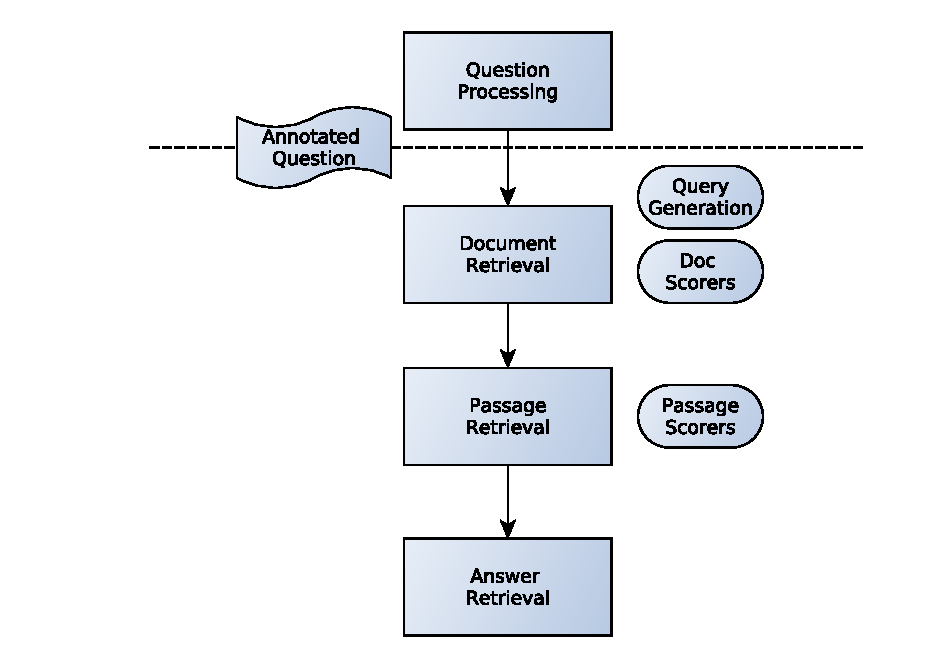
\includegraphics[scale=0.75]{graficos/AnswerRetrievalFlowWiki}
%   \caption{Flow para la Generación de Respuestas - No Estructurado}
%   \label{fig:AnswerRetrievalFlowWiki}
% \end{figure}

% \subsubsection{Documentos}
% \label{subsec:docs}
% En este punto, para una pregunta dada se dispone de la entidad del grupo de preguntas y de las distintas anotaciones hechas a la pregunta en el paso anterior (\allref{sec:qprocess}). Por su parte, los documentos en los índices invertidos poseen los campos $Id$, $Title$, y $Text$. El mecanismo de generación de queries tiene como objetivo priorizar en el ranking los documentos relacionados con el tema asociado al grupo de preguntas. Este paso es un problema de information retrieval puro: esto es, dado un pedido de información, retornar \textit{documentos relevantes}. El análisis semántico tiene peso en el paso posterior, a la hora de rankear pasajes. Por ejemplo, para el primer grupo de preguntas acerca de Harry Potter, solo se espera de este una lista de de documentos relacionados con ese mundo, en primer lugar. Por otro lado, es necesario que los principios de generación de queries no sean demasiado estrictos. Si en este punto quedan afuera muchas ocurrencias de una respuesta, entonces todo el resto del programa se ve afectado de manera irreparable. Es preferible generar documentos de más y luego filtrarlos mediante análisis lingüístico que ser demasiado estrictos y perder respuestas.
% Para lograr esto, ponderamos los documentos en los que las entidades nombradas reconocidas lingüísticamente aparecen en el título, si se dispone de más de una entidad buscamos documentos que mencionen ambos, luego priorizamos los documentos que poseen estas entidades dentro del cuerpo y también consideramos la presencia de verbos en diferentes conjugaciones y de sustantivos que ocurren en la pregunta. Finalmente, agregamos una lista de documentos enviando la pregunta misma como una query.

% Dado que finalmente se realizan queries simples (masivas), cabe preguntarse cual es la razón de la generación de queries y la ponderación de documentos. Esta razón es que en el proceso de ranking de pasajes y evaluación de respuesta se utilizan features basados en el score dado por lucene a los diferentes documentos. Si una mejor posición del documento contenedor del pasaje no implica que el pasaje sea correcto, si en cambio es un indicador de que dicho pasaje se encontró más cerca o más lejos del nucleo temático en el que se esperaba encontrarlo.

% Una vez generada la lista de documentos rankeados según lucene, se procede a analizar algunos features en base a distintos scorers propios. A su vez, estos distintos valores se combinan en una evaluación general del documento, que será utilizada luego a la hora de generar una respuesta. Estas dimensiones buscan en el título y en el artículo diferente medidas sobre las entidades nombradas y sobre la pregunta completa. En concreto, se miden distancias a la entidad nombrada que identifica al grupo de preguntas (ver \allref{subsec:entidad-de-grupo}), las entidades nombradad en la pregunta misma, a la pregunta completa y la respuesta esperada data. Las medidas contra la respuesta esperada -dada por Clef- no pueden usarse para generar la respuesta, pero sí para evaluar la performance del sistema. En el siguiente cuadro se muestran las dimensiones que se consideran sobre los documentos.

% \begin{center}
% \begin{tabular}{| l | l | l |}
% \hline
% Entidad & Campo & Comparador \\ \hline
% \multirow{6}{*}{Entidad de Grupo} & \multirow{3}{*}{Título} & Span \\
% & & Covr \\
% & & Freq \\ \cline{2-3}
% & \multirow{3}{*}{Texto} & Span \\
% & & Covr \\
% & & Freq \\ \hline
% \multirow{6}{*}{Entidades de Pregunta} & \multirow{3}{*}{Título} & Span \\
% & & Covr \\
% & & Freq \\ \cline{2-3}
% & \multirow{3}{*}{Texto} & Span \\
% & & Covr \\
% & & Freq \\ \hline
% \multirow{6}{*}{Todas las entidades} & \multirow{3}{*}{Título} & Span \\
% & & Covr \\
% & & Freq \\ \cline{2-3}
% & \multirow{3}{*}{Texto} & Span \\
% & & Covr \\
% & & Freq \\ \hline
% \multirow{6}{*}{Pregunta} & \multirow{3}{*}{Título} & Span \\
% & & Covr \\
% & & Freq \\ \cline{2-3}
% & \multirow{3}{*}{Texto} & Span \\
% & & Covr \\
% & & Freq \\ \hline
% \multirow{6}{*}{Respuesta} & \multirow{3}{*}{Título} & Span \\
% & & Covr \\
% & & Freq \\ \cline{2-3}
% & \multirow{3}{*}{Texto} & Span \\
% & & Covr \\
% & & Freq \\ \hline
% Score según índice & -- & -- \\ \hline
% \end{tabular}
% \end{center}

% Los comparadores señalados ($Freq$, $Covr$, y $Span$) se utilizan en distintos lugares de esta tesis y su funcionamiento es explicado en el apéndice \allref{sec:comparadores}. Notar que `Entidades de la pregunta' refiere tanto a aquellas reconocidas por el NER-tagger como a construcciones sustantivadas y que `Pregunta' no es la pregunta bruta sino la priorización de verbos conjugados, sustantivos, adjetivos y entidades.

% El score general del documento es un cálculo ponderado de estas diferentes dimensiones.

% Lucene permite especificar cuántos documentos queremos recuperar. Para evaluar la performance de este paso, utilizamos medida distintos scores en base a la respuesta dada por dada por la conferencia para el ejercicio. Es importante notar que dado que no utilizamos las imagenes de wikipedia de la primera sugerencia, es esperable que las respuesta no estén `tal cual'.
% Evaluamos distintos mecanismos de generación de documentos, con distinta cantidad total, bajo distintas métricas. Para generar documentos, probamos la query trivial $ALL: pregunta$ (1), una un poco mejorada $ALL: entidad_de_grupo pregunta$ (2), secuencias concatenadas de queries tal como las describimos más arriba (3) y varios pedidos separados aplanados en un paso posterior (4). Para los cuatro métodos eliminamos los signos de puntuación. Para medir los resultados, utilizamos los comparadores de presencia exacta y diferentes grados de cobertura de términos (.8, .9 y 1). A su vez, evaluamos distintas imagenes de wikipedia para el español. Es total de preguntas del ejercicio, recordamos, es 200. Los resultados son los siguientes.

% \begin{center}
% \begin{tabular}{|l|l|l|l|l|l|l|}
% \hline
% Método & \# Docs & Wikipedia & Exacto & Covr 1 & Covr .9 & Covr . 8 \\ \hline

% \multirow{6}{*}{1 - Trivial} &
% \multirow{3}{*}{100} & es - 2006 & 132 & 151 & 152 & 159 \\
%  &  & es - 2007 & 144 & 159 & 160 & 164 \\
%  &  & en - 2006 & x & x & x & x \\ \cline{2-7}
%  & \multirow{3}{*}{1000} & es - 2006 & 144 & 167 & 167 & 173 \\
%  &  & es - 2007 & 159 & 177 & 177 & 180 \\
%  &  & en - 2006 & x & x & x & x \\ \hline

% \multirow{6}{*}{2 - Trivial'} &
% \multirow{3}{*}{100} & es - 2006 & 138 & 156 & 157 & 164 \\
%  &  & es - 2007 & 151 & 167 & 168 & 171 \\
%  &  & en - 2006 & x & x & x & x \\ \cline{2-7}
%  & \multirow{3}{*}{1000} & es - 2006 & 147 & 168 & 168 & 174 \\
%  &  & es - 2007 & 163 & 178 & 178 & 181 \\
%  &  & en - 2006 & x & x & x & x \\ \hline
% hola & ey &wiki& 137 & 156 & 157 & 160  \\ \hline
% \multirow{6}{*}{3 - Inteligente} &
% \multirow{3}{*}{100} & es - 2006 & 127 & 144 & 144 & 150 \\
%  &  & es - 2007 & 141 & 150 & 151 & 156 \\
%  &  & en - 2006 & x & x & x & x \\ \cline{2-7}

%  & \multirow{3}{*}{1000} & es - 2006 & 143 & 163 & 163 & 170 \\
%  &  & es - 2007 & 158 & 175 & 175 & 179 \\
%  &  & en - 2006 & x & x & x & x \\ \hline

% \multirow{6}{*}{4 - Inteligente'} &
% \multirow{3}{*}{100} & es - 2006 & 142 & 160 & 161 & 168 \\
%  &  & es - 2007 & 157 & 170 & 171 & 174  \\
%  &  & en - 2006 & x & x & x & x \\ \cline{2-7}


%  & \multirow{3}{*}{1000} & es - 2006 & 147 & 168 & 168 & 174 \\
%  &  & es - 2007 & x & 158 & x & x \\
%  &  & en - 2006 & x & x & x & x \\ \hline

% \end{tabular}
% \end{center}

% Conclusión de esto.

% \subsubsection{Pasajes}
% Este paso es análogo al anterior, pero con mayor detalle y granularidad. Cada documento generado en el paso anterior, con sus diferentes puntajes para
% las dimensiones señaladas, se parten en pasajes u oraciones. Nuevamente, sobre estas oraciones realizamos diferentes mediciones y las combinamos generando
% un score final. En esta sección discutiremos las mediciones consideradas y los diferentes métodos de combinación de las mismas. Estos métodos de combinación generan distintos rankings de pasajes. Para evaluar estos rankings, nuevamente, utilizaremos la información disponible sobre las respuestas esperadas, buscando que la respuesta esperada se encuentre entre los $n$ pasajes mejor rankeados.
% En primer lugar, las distintos scorers implementados son los siguientes:

% \begin{center}
% \begin{tabular}{| l | l | l |}
% \hline
% Comparador & Qué & Dónde \\ \hline
% \multicolumn{3}{|c|}{Estadísticos} \\ \hline
% Freq & Pregunta & Pasaje \\ \hline
% Span & Pregunta & Pasaje \\ \hline
% Covr & Pregunta & Pasaje \\ \hline
% \#Tokens & -- & Pasaje \\ \hline
% \multicolumn{3}{|c|}{Basados en NLP} \\ \hline
% Presencia & Entidad de Grupo & Pasaje \\ \hline
% Presencia & Entidades de pregunta & Pasaje \\ \hline
% Presencia & Verbos de pregunta & Pasaje \\ \hline
% Presencia & Sustantivos de pregunta & Pasaje \\ \hline
% \multicolumn{3}{|c|}{Para evaluación} \\ \hline
% Freq & Respuesta & Pasaje \\ \hline
% Span & Respuesta & Pasaje \\ \hline
% Covr & Respuesta & Pasaje \\ \hline
% \end{tabular}
% \end{center}

% A estos Scorers se le suman los scores del documento asociado al pasaje (ver \allref{subsec:docs}).
% Sobre estas dimensiones disponibles, intentamos las siguientes combinaciones de priorización:

% \begin{center}
% \begin{tabular}{|l|l|l|}
% \hline
% \#& Nombre & Fórmula \\ \hline
% 1& Simple & $2+2=4$ \\ \hline
% 2& Respuesta & $2+2=4$ \\ \hline
% 3& Compleja & $2+2=4$ \\ \hline
% \end{tabular}
% \end{center}

% Y consideramos la ocurrencia de respuestas, de la misma manera que en el apartado anterior (Match Exacto y tres medidas de covertura de tokens: 1, .9 y .8),
% sobre los primeros $n$ pasajes, con $n$ = 1, 5, 10, 20, 50 y 100.

% \begin{center}
% \begin{tabular}{|l|l|l|l|l|l|}
% \hline
% Fórmula & \#Docs & Exacto & Covr 1 & Covr .9 & Covr . 8 \\ \hline
% \multirow{6}{*}{1} & 1 & x & x & x & x \\  \cline{2-6}
%  & 5 & x & x & x & x \\ \cline{2-6}
%  & 10 & x & x & x & x \\ \cline{2-6}
%  & 20 & x & x & x & x \\ \cline{2-6}
%  & 50 & x & x & x & x \\ \cline{2-6}
%  & 100 & x & x & x & x \\ \hline
% \end{tabular}
% \end{center}


% \subsubsection{Respuestas}





% \begin{figure}
%   \centering
%     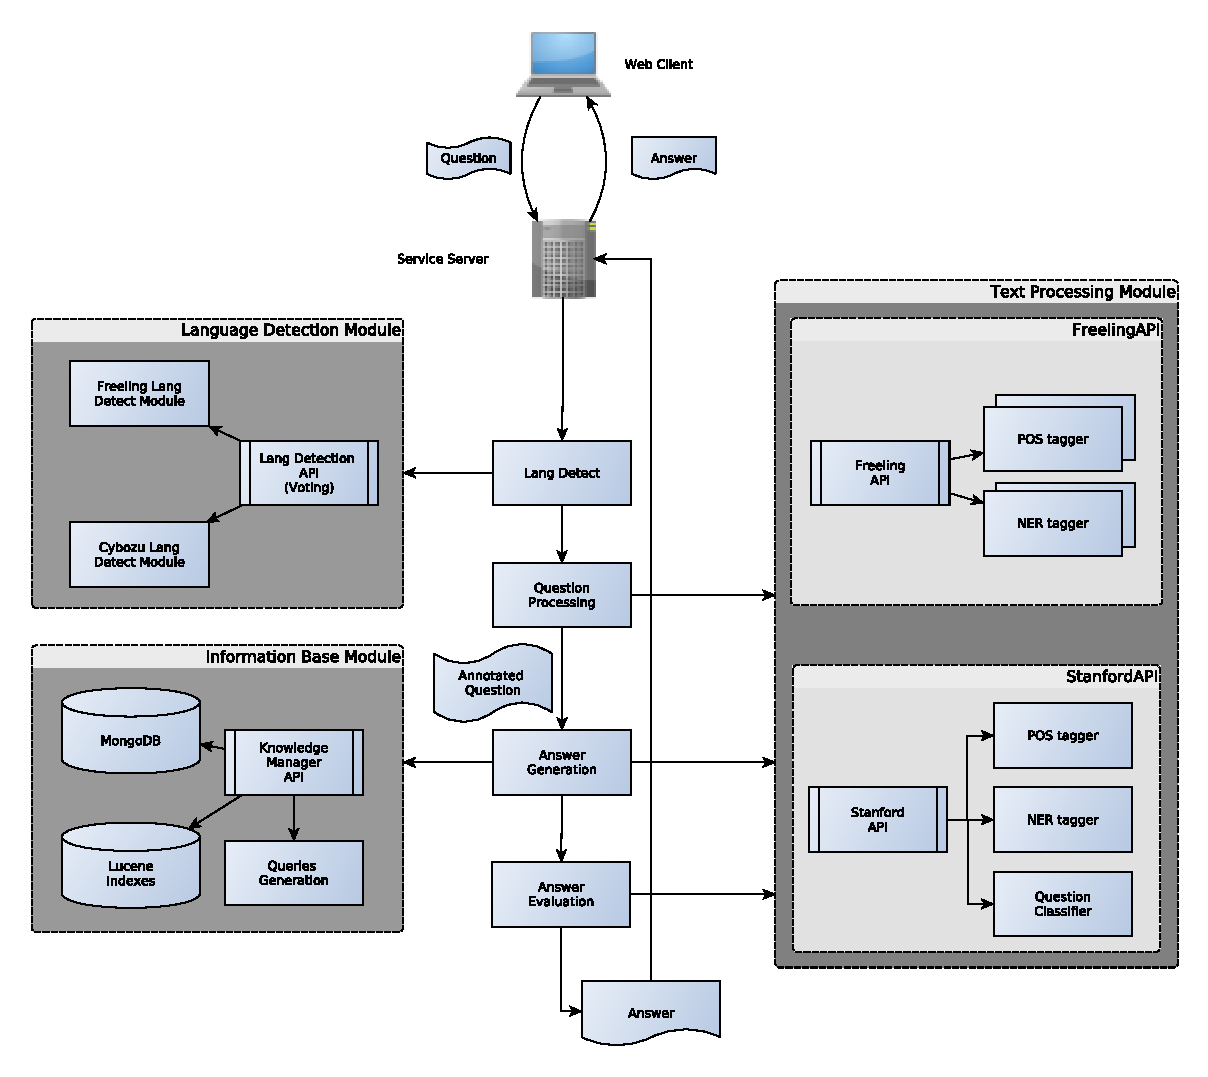
\includegraphics[scale=0.86]{graficos/Architecture}
%   \caption{Arquitectura}
%   \label{fig:Architecture}
% \end{figure}

% %\end{document}


% \appendix
\nocite{*}

\begin{appendices}
  \appendix
\chapter{Herramientas}
\label{chap:herramientas}

\section{Stanford Question Classifier}
\label{sec:stanford-qc}
El Question Classifier de Stanford \cite{QC2} es un sistema de clasificación de preguntas basado en machine learning que utiliza la arquitectura de aprendizaje SNoW. Es un sistema jerárquico guiado por una semántica de dos niveles que permite la clasificación en categorías granulares. Según los tests de los autores, el proceso logra una efectividad del 90\% sobre 50 diferentes clases finales, utilizando features sintácticos y semánticos.

El clasificador dispone de una taxonomía de dos capas basada en los tipos de respuesta típicos de la TREC. Las clases superiores son seis: abreviatura, entidad, descripción, humano, lugar y numérico; divididas a su vez en 50 subclases más finas no solapadas (50 en total). La motivación de la existencia de clases superiores es doble: por un lado, ellas preservan compatibilidad y coherencia con las clases usadas en trabajos previos de clasificación de preguntas. Por otro, se esperaba obtener mejoras de performance aplicando dos fases de clasificación, pero esta intención no se corroboró en la experiencia

La tabla siguiente muestra la taxonomía de clasificación dividida en clases y subclases \footnote{Puede encontrarse en esta url: \url{http://cogcomp.cs.illinois.edu/Data/QA/QC/definition.html} y está explicada en \cite{QC2} y \cite{QC3}}


\begin{center}
\begin{longtable}{| l | l |}
\hline
Clase y subclase & Definición \\ \hline
ABBREVIATION &  abbreviation \\ \hline
  abb & abbreviation\\ \hline
  exp & expression abbreviated\\ \hline
ENTITY  & entities\\ \hline
  animal  & animals\\ \hline
  body & organs of body\\ \hline
  color & colors\\ \hline
  creative & inventions, books and other creative pieces\\ \hline
  currency & currency names\\ \hline
  dis.med. & diseases and medicine\\ \hline
  event & events\\ \hline
  food & food\\ \hline
  instrument & musical instrument\\ \hline
  lang & languages\\ \hline
  letter & letters like a-z\\ \hline
  other & other entities\\ \hline
  plant & plants\\ \hline
  product & products\\ \hline
  religion  & religions\\ \hline
  sport & sports\\ \hline
  substance & elements and substances\\ \hline
  symbol & symbols and signs\\ \hline
  technique & techniques and methods\\ \hline
  term  & equivalent terms\\ \hline
  vehicle & vehicles\\ \hline
  word & words with a special property\\ \hline
DESCRIPTION & description and abstract concepts\\ \hline
  definition & definition of sth.\\ \hline
  description & description of sth.\\ \hline
  manner & manner of an action\\ \hline
  reason & reasons\\ \hline
%\end{tabular}
%\begin{tabular}{| l | l |}
%\hline
HUMAN & human beings\\ \hline
  group & a group or organization of persons\\ \hline
  ind & an individual\\ \hline
  title & title of a person\\ \hline
  description & description of a person\\ \hline
LOCATION & locations\\ \hline
  city & cities\\ \hline
  country & countries\\ \hline
  mountain & mountains\\ \hline
  other & other locations\\ \hline
  state & states\\ \hline
NUMERIC & numeric values\\ \hline
  code  & postcodes or other codes\\ \hline
  count & number of sth.\\ \hline
  date  & dates\\ \hline
  distance &  linear measures\\ \hline
  money & prices\\ \hline
  order & ranks\\ \hline
  other & other numbers\\ \hline
  period  & the lasting time of sth.\\ \hline
  percent & fractions\\ \hline
  speed & speed\\ \hline
  temp & temperature\\ \hline
  size & size, area and volume\\ \hline
  weight & weight\\ \hline
\end{longtable}
\end{center}


Uno de los principales problemas que tuvieron los autores al enfrentarse a clases tan específicas fue la ambigüedad instrínseca de ciertas preguntas. Los siguientes ejemplos de este problema están tomados de \cite{QC2}:
\begin{itemize}
\item What is bipolar disorder? (¿Qué es el desorden bipolar?)
\item What do bats eat? (¿Qué comen los murciélagos?)
\end{itemize}
La primer pregunta puede pertenecer a la clase \textit{definición} o bien a la clase \textit{enfermedad / medicina} y la segunda a \textit{comida}, \textit{planta} o \textit{animal}. Para abordar este problema, el clasificador asigna diferentes clases ponderadas y no una única clase.

Los dos niveles de clasificación están implementados como dos clasificadores simples en secuencia, ambos utilizando el algoritmo Winnow de SNoW. El primero etiqueta la pregunta en función de las clases más generales y el segundo asigna las clases más finas (dentro de las suclases determinadas por la clase del primero).
El modelo para el algoritmo de aprendizaje representa las preguntas como listas de características (\textit{features}) tanto sintácticos como semánticos. Los features utilizando son, en total, más de 200.000, siendo casi todos combinaciones complejas de un set acotado de features simples basados en palabras, pos tags, chunks (componentes constitucionales de la oración), chunks principales (por ejemplo: componente nominal principal), entidades nombradas y palabras semánticamente relacionadas a ciertas clases. De estos seis tipos de features primitivos, tres son sintácticos (pos tags, chunks, chunks principales) mientras que otros son semánticos (named entities, palabras relacionadas).

El clasificador, al igual que el resto de las herramientas de nlp de Stanford, está implementado en java.


\section{Stanford POS \& NER Taggers}
\label{sec:stanford-pos}
\label{sec:stanford-both}
El POS tagger de Stanford es un algortimo basado en entropía máxima (\textit{maximum entropy}), implementado en java originalmente en \cite{POS2}, con algunos agregados y mejoras técnicas realizadas en \cite{POS1}. Al descargar el paquete, también está disponible uno más complejo con soporte para los idiomas árabe, chino y alemán. En este trabajo utilizamos el paquete sencillo, que consta de dos modelos entrenados para inglés, usando, como señalamos en \allref{subsec:pos} el tagset de Penn Treebank.


Por su parte, el NER tagger de Stanford, es una implementación general de

It comes with well-engineered feature extractors for Named Entity Recognition, and many options for defining feature extractors. Included with the download are good named entity recognizers for English, particularly for the 3 classes (PERSON, ORGANIZATION, LOCATION), and we also make available on this page various other models for different languages and circumstances, including models trained on just the CoNLL 2003 English training data. The distributional similarity features in some models improve performance but the models require considerably more memory.

Stanford NER is also known as CRFClassifier. The software provides a general implementation of (arbitrary order) linear chain Conditional Random Field (CRF) sequence models. That is, by training your own models, you can actually use this code to build sequence models for any task. (CRF models were pioneered by Lafferty, McCallum, and Pereira (2001); see Sutton and McCallum (2006) or Sutton and McCallum (2010) for more comprehensible introductions.)

The CRF code is by Jenny Finkel. The feature extractors are by Dan Klein, Christopher Manning, and Jenny Finkel. Much of the documentation and usability is due to Anna Rafferty. The CRF sequence models provided here do not precisely correspond to any published paper, but the correct paper to cite for the software is:

Jenny Rose Finkel, Trond Grenager, and Christopher Manning. 2005. Incorporating Non-local Information into Information Extraction Systems by Gibbs Sampling. Proceedings of the 43nd Annual Meeting of the Association for Computational Linguistics (ACL 2005), pp. 363-370. http://nlp.stanford.edu/~manning/papers/gibbscrf3.pdf
The software provided here is similar to the baseline local+Viterbi model in that paper, but adds new distributional similarity based features (in the -distSim classifiers). The big models were trained on a mixture of CoNLL, MUC-6, MUC-7 and ACE named entity corpora, and as a result the models are fairly robust across domains.
Named Entity Recognition Stanford Named Entity Recognizer (Finkel,
Grenager and Manning 2005)

Finkel, Jenny Rose, Trond Grenager, and Christopher Manning. "Incorporating
Non-local Information into Information Extraction Systems by Gibbs Sampling."
roceedings of the 43nd Annual Meeting of the Association for Computational
Linguistics. 2005.



\section{Freeling}
\label{sec:freeling}
\label{subsec:freeling-pos}
\label{subsec:freeling-mods}
Freeling es una librería de c\'odigo abierto que provee distintas herramientas de
procesamiento de lenguaje natural, desarrollada y mantenida por el Centre de Tecnologies
i Aplicacions del Llenguatge i la Parla (TALP) de la Universidad Politécnica de Catalu\~na (UPC).
Freeling está dise\~nado para ser usada como una librería externa y ofrece un API en distintos lenguajes
de programaci\'on. Su principal virtud es ser multilingüe, esto es, los diferentes analizadores que provee funcionan
para un conjunto bastante amplio de idiomas. La última versi\'on a la fecha (3.1) soporta los siguientes idiomas:

\begin{itemize}
\item Asturian (as)
\item Catalan (ca)
\item English (en)
\item French (fr)
\item Galician (gl)
\item Italian (it)
\item Portuguese (pt)
\item Russian (ru)
\item Slovene (sl)
\item Spanish (es)
\item Welsh (cy)
\end{itemize}

Cabe destacar que no todos los m\'odulos soportan todos los idiomas. Sin embargo, dado que el proyecto está radicado en Espa\~na,
los idiomas necesarios para los fines de nuestro trabajo (espa\~nol e inglés), soportan todos los m\'odulos disponibles
en la librería.
Freeling 3.1 ofrece los siguientes analizadores lingüisticos:

\begin{itemize}
\item Detecci\'on de idioma
\item Tokenizer
\item Sentence splitting,
\item Análisis morfol\'ogico
\item NER y NEC (Detecci\'on y Clasificaci\'on de Entidades Nombradas)
\item Reconocimiento de fechas, números, magnitudes físicas, monedas
\item Codificaci\'on fonética
\item POS tagging,
\item Shallow parsing
\item Dependency parsing
\item Wordnet-based sense annotation
\item Word Sense Disambiguation
\item Coreference resolution
\end{itemize}


El módulo de POS tagging de Freeling dispone de dos tagger. El primero, $hmm\_tagger$, es un algoritmo clásico que utiliza Hidden Markov Models (HMMs) con tri-gramas. La descripción del algoritmo de tagging basado en HMM se encuentra con detalle en  en \cite{POS0}. Por otro lado, el módulo incorpora un método llamado $relax\_tagger$ que permite la creación de un sistema híbrido que permite reglas escritas a mano y modelos estadísticos.

\section{Apache Lucene}
\label{sec:lucene}
Lucene es una librería de information retrieval, de c\'odigo abierto, escrita en Java y distribuida
bajo la licencia Apache Software License por la Apache Software Foundation. No está pensada para
usuarios finales sino para ser integrada dentro de proyectos informáticos, resolviendo
la parte de bajo nivel y brindando servicios a través de un API en diferentes lenguajes de programaci\'on.
Su core es un índice invertido como el que describimos anteriormente. La implementaci\'on de un sistema
que utiliza Lucene consta de dos pasos separados:
\begin{itemize}
\item La \textbf{creaci\'on} del índice, es por lo general un proceso offline en el cual
se incorporan distintas fuentes de informaci\'on al índice
\item La \textbf{búsqueda} de documentos en el índice creado en el paso anterior, a partir de una query
ingresada por el usuario final. Este proceso se incorpora dentro del flujo `online' del sistema.
El resultado de esta búsqueda es una lista de documentos rankeados con un cierto puntaje.
\end{itemize}

Es importante señalar que si bien el proceso de creaci\'on del índice suele estar desacoplado del resto
del sistema, las fuentes de informaci\'on no tiene por que ser `offline' en el sentido de ser documentos
en un disco local. De hecho, Nutch, otro proyecto de c\'odigo abierto de la Apache Software Foundation es
un motor de búsqueda web basado en Lucene que incorpora un crawler para indexar sitios web. Lucene soporta
cualquier fuente de informaci\'on que pueda convertirse en texto mediante algoritmia.
\newline
Los conceptos fundamentales de Lucene son: índice, documento, campo, término y query.
\begin{itemize}
\item Un índice contiene un conjunto de documentos
\item Un documento es un conjunto de campos
\item Un campo es el nombre de una secuencia de términos
\item Un término es un token (una palabra)
\item Una query es una lista de términos conectados con distintos operados l\'ogicos
\end{itemize}
\end{appendices}

%%%% BIBLIOGRAFIA
\backmatter
\bibliographystyle{apalike}
\cleardoublepage
\phantomsection
\addcontentsline{toc}{chapter}{Bibliografía}
\bibliography{tesis}


\end{document}
